\documentclass[twoside]{book}

% Packages required by doxygen
\usepackage{fixltx2e}
\usepackage{calc}
\usepackage{doxygen}
\usepackage[export]{adjustbox} % also loads graphicx
\usepackage{graphicx}
\usepackage[utf8]{inputenc}
\usepackage{makeidx}
\usepackage{multicol}
\usepackage{multirow}
\PassOptionsToPackage{warn}{textcomp}
\usepackage{textcomp}
\usepackage[nointegrals]{wasysym}
\usepackage[table]{xcolor}

% Font selection
\usepackage[T1]{fontenc}
\usepackage[scaled=.90]{helvet}
\usepackage{courier}
\usepackage{amssymb}
\usepackage{sectsty}
\renewcommand{\familydefault}{\sfdefault}
\allsectionsfont{%
  \fontseries{bc}\selectfont%
  \color{darkgray}%
}
\renewcommand{\DoxyLabelFont}{%
  \fontseries{bc}\selectfont%
  \color{darkgray}%
}
\newcommand{\+}{\discretionary{\mbox{\scriptsize$\hookleftarrow$}}{}{}}

% Page & text layout
\usepackage{geometry}
\geometry{%
  a4paper,%
  top=2.5cm,%
  bottom=2.5cm,%
  left=2.5cm,%
  right=2.5cm%
}
\tolerance=750
\hfuzz=15pt
\hbadness=750
\setlength{\emergencystretch}{15pt}
\setlength{\parindent}{0cm}
\setlength{\parskip}{3ex plus 2ex minus 2ex}
\makeatletter
\renewcommand{\paragraph}{%
  \@startsection{paragraph}{4}{0ex}{-1.0ex}{1.0ex}{%
    \normalfont\normalsize\bfseries\SS@parafont%
  }%
}
\renewcommand{\subparagraph}{%
  \@startsection{subparagraph}{5}{0ex}{-1.0ex}{1.0ex}{%
    \normalfont\normalsize\bfseries\SS@subparafont%
  }%
}
\makeatother

% Headers & footers
\usepackage{fancyhdr}
\pagestyle{fancyplain}
\fancyhead[LE]{\fancyplain{}{\bfseries\thepage}}
\fancyhead[CE]{\fancyplain{}{}}
\fancyhead[RE]{\fancyplain{}{\bfseries\leftmark}}
\fancyhead[LO]{\fancyplain{}{\bfseries\rightmark}}
\fancyhead[CO]{\fancyplain{}{}}
\fancyhead[RO]{\fancyplain{}{\bfseries\thepage}}
\fancyfoot[LE]{\fancyplain{}{}}
\fancyfoot[CE]{\fancyplain{}{}}
\fancyfoot[RE]{\fancyplain{}{\bfseries\scriptsize Generated by Doxygen }}
\fancyfoot[LO]{\fancyplain{}{\bfseries\scriptsize Generated by Doxygen }}
\fancyfoot[CO]{\fancyplain{}{}}
\fancyfoot[RO]{\fancyplain{}{}}
\renewcommand{\footrulewidth}{0.4pt}
\renewcommand{\chaptermark}[1]{%
  \markboth{#1}{}%
}
\renewcommand{\sectionmark}[1]{%
  \markright{\thesection\ #1}%
}

% Indices & bibliography
\usepackage{natbib}
\usepackage[titles]{tocloft}
\setcounter{tocdepth}{3}
\setcounter{secnumdepth}{5}
\makeindex

% Hyperlinks (required, but should be loaded last)
\usepackage{ifpdf}
\ifpdf
  \usepackage[pdftex,pagebackref=true]{hyperref}
\else
  \usepackage[ps2pdf,pagebackref=true]{hyperref}
\fi
\hypersetup{%
  colorlinks=true,%
  linkcolor=blue,%
  citecolor=blue,%
  unicode%
}

% Custom commands
\newcommand{\clearemptydoublepage}{%
  \newpage{\pagestyle{empty}\cleardoublepage}%
}

\usepackage{caption}
\captionsetup{labelsep=space,justification=centering,font={bf},singlelinecheck=off,skip=4pt,position=top}

%===== C O N T E N T S =====

\begin{document}

% Titlepage & ToC
\hypersetup{pageanchor=false,
             bookmarksnumbered=true,
             pdfencoding=unicode
            }
\pagenumbering{alph}
\begin{titlepage}
\vspace*{7cm}
\begin{center}%
{\Large Telemetry Firmware }\\
\vspace*{1cm}
{\large Generated by Doxygen 1.8.14}\\
\end{center}
\end{titlepage}
\clearemptydoublepage
\pagenumbering{roman}
\tableofcontents
\clearemptydoublepage
\pagenumbering{arabic}
\hypersetup{pageanchor=true}

%--- Begin generated contents ---
\chapter{Class Index}
\section{Class List}
Here are the classes, structs, unions and interfaces with brief descriptions\+:\begin{DoxyCompactList}
\item\contentsline{section}{\mbox{\hyperlink{class_i2_c_manager}{I2\+C\+Manager}} \\*Responsible for discovering the connectivity status of I2C peripherals }{\pageref{class_i2_c_manager}}{}
\item\contentsline{section}{\mbox{\hyperlink{class_i2_c_peripheral_manager}{I2\+C\+Peripheral\+Manager}} \\*Manages all the read managers and memory allocation for a single peripheral }{\pageref{class_i2_c_peripheral_manager}}{}
\item\contentsline{section}{\mbox{\hyperlink{class_i2_c_read_manager}{I2\+C\+Read\+Manager}} \\*Responsible for a state machine which reads data from the I2C bus in a non-\/blocking fashion }{\pageref{class_i2_c_read_manager}}{}
\item\contentsline{section}{\mbox{\hyperlink{class_i2_c_runtime}{I2\+C\+Runtime}} \\*Responsible for the primary event loop for all peripherals on the bus }{\pageref{class_i2_c_runtime}}{}
\item\contentsline{section}{\mbox{\hyperlink{class_m_q_t_t_manager}{M\+Q\+T\+T\+Manager}} \\*Responsible for publishing and subscribing to topics on the M\+Q\+TT broker }{\pageref{class_m_q_t_t_manager}}{}
\item\contentsline{section}{\mbox{\hyperlink{struct_peripheral}{Peripheral}} \\*Declarative configuration for the behaviour of a peripheral on the I2C bus }{\pageref{struct_peripheral}}{}
\item\contentsline{section}{\mbox{\hyperlink{struct_peripheral_status}{Peripheral\+Status}} \\*Intermediate object for protobuf encoding }{\pageref{struct_peripheral_status}}{}
\item\contentsline{section}{\mbox{\hyperlink{struct_read_definition}{Read\+Definition}} \\*Declarative configuration for reading a contiguous register block from a peripheral on the I2C bus }{\pageref{struct_read_definition}}{}
\item\contentsline{section}{\mbox{\hyperlink{struct_schedule}{Schedule}} \\*Declarative configuration for a managed schedule }{\pageref{struct_schedule}}{}
\item\contentsline{section}{\mbox{\hyperlink{class_scheduler}{Scheduler}} \\*Generic scheduler for non-\/blocking tasks given schedules for callbacks }{\pageref{class_scheduler}}{}
\item\contentsline{section}{\mbox{\hyperlink{struct_setup_write_definition}{Setup\+Write\+Definition}} }{\pageref{struct_setup_write_definition}}{}
\item\contentsline{section}{\mbox{\hyperlink{struct_sized}{Sized}} \\*Buffer/size pair }{\pageref{struct_sized}}{}
\item\contentsline{section}{\mbox{\hyperlink{class_telemetry_protocol}{Telemetry\+Protocol}} \\*Responsible for encoding and decoding protobuf/nanopb payloads }{\pageref{class_telemetry_protocol}}{}
\item\contentsline{section}{\mbox{\hyperlink{class_wi_fi_provisioning}{Wi\+Fi\+Provisioning}} \\*Manages the web application for provisioning connectivity information }{\pageref{class_wi_fi_provisioning}}{}
\end{DoxyCompactList}

\chapter{File Index}
\section{File List}
Here is a list of all files with brief descriptions\+:\begin{DoxyCompactList}
\item\contentsline{section}{include/\mbox{\hyperlink{_i2_c_manager_8h}{I2\+C\+Manager.\+h}} }{\pageref{_i2_c_manager_8h}}{}
\item\contentsline{section}{include/\mbox{\hyperlink{_i2_c_peripheral_8h}{I2\+C\+Peripheral.\+h}} }{\pageref{_i2_c_peripheral_8h}}{}
\item\contentsline{section}{include/\mbox{\hyperlink{_i2_c_read_manager_8h}{I2\+C\+Read\+Manager.\+h}} }{\pageref{_i2_c_read_manager_8h}}{}
\item\contentsline{section}{include/\mbox{\hyperlink{_i2_c_runtime_8h}{I2\+C\+Runtime.\+h}} }{\pageref{_i2_c_runtime_8h}}{}
\item\contentsline{section}{include/\mbox{\hyperlink{_m_q_t_t_manager_8h}{M\+Q\+T\+T\+Manager.\+h}} }{\pageref{_m_q_t_t_manager_8h}}{}
\item\contentsline{section}{include/\mbox{\hyperlink{_scheduler_8h}{Scheduler.\+h}} }{\pageref{_scheduler_8h}}{}
\item\contentsline{section}{include/\mbox{\hyperlink{_telemetry_protocol_8h}{Telemetry\+Protocol.\+h}} }{\pageref{_telemetry_protocol_8h}}{}
\item\contentsline{section}{include/\mbox{\hyperlink{_wi_fi_provisioning_8h}{Wi\+Fi\+Provisioning.\+h}} }{\pageref{_wi_fi_provisioning_8h}}{}
\item\contentsline{section}{src/\mbox{\hyperlink{_i2_c_manager_8cpp}{I2\+C\+Manager.\+cpp}} }{\pageref{_i2_c_manager_8cpp}}{}
\item\contentsline{section}{src/\mbox{\hyperlink{_i2_c_read_manager_8cpp}{I2\+C\+Read\+Manager.\+cpp}} }{\pageref{_i2_c_read_manager_8cpp}}{}
\item\contentsline{section}{src/\mbox{\hyperlink{_i2_c_runtime_8cpp}{I2\+C\+Runtime.\+cpp}} }{\pageref{_i2_c_runtime_8cpp}}{}
\item\contentsline{section}{src/\mbox{\hyperlink{main_8cpp}{main.\+cpp}} }{\pageref{main_8cpp}}{}
\item\contentsline{section}{src/\mbox{\hyperlink{_m_q_t_t_manager_8cpp}{M\+Q\+T\+T\+Manager.\+cpp}} }{\pageref{_m_q_t_t_manager_8cpp}}{}
\item\contentsline{section}{src/\mbox{\hyperlink{_scheduler_8cpp}{Scheduler.\+cpp}} }{\pageref{_scheduler_8cpp}}{}
\item\contentsline{section}{src/\mbox{\hyperlink{_telemetry_protocol_8cc}{Telemetry\+Protocol.\+cc}} }{\pageref{_telemetry_protocol_8cc}}{}
\item\contentsline{section}{src/\mbox{\hyperlink{_wi_fi_provisioning_8cpp}{Wi\+Fi\+Provisioning.\+cpp}} }{\pageref{_wi_fi_provisioning_8cpp}}{}
\end{DoxyCompactList}

\chapter{Class Documentation}
\hypertarget{class_i2_c_manager}{}\section{I2\+C\+Manager Class Reference}
\label{class_i2_c_manager}\index{I2\+C\+Manager@{I2\+C\+Manager}}


Responsible for discovering the connectivity status of I2C peripherals.  




{\ttfamily \#include $<$I2\+C\+Manager.\+h$>$}



Collaboration diagram for I2\+C\+Manager\+:\nopagebreak
\begin{figure}[H]
\begin{center}
\leavevmode
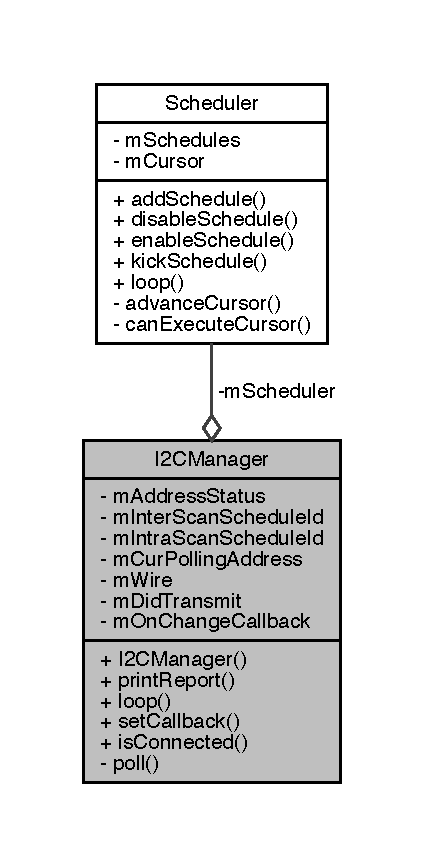
\includegraphics[width=203pt]{class_i2_c_manager__coll__graph}
\end{center}
\end{figure}
\subsection*{Public Member Functions}
\begin{DoxyCompactItemize}
\item 
\mbox{\hyperlink{class_i2_c_manager_a2d806ad3a65969077b436f0d3a9a70f2}{I2\+C\+Manager}} (Two\+Wire $\ast$\mbox{\hyperlink{main_8cpp_ab8d8f9af97a698a5a73132c347acbaf4}{wire}}, \mbox{\hyperlink{_scheduler_8h_aca1fa1a7edde6bf9e22c7617400fad31}{Duration}} inter\+Scan\+Period=\mbox{\hyperlink{_i2_c_manager_8h_a5aa8afc0ad4792d13a6cb089c9d50537}{I2\+C\+M\+A\+N\+A\+G\+E\+R\+\_\+\+D\+E\+F\+A\+U\+L\+T\+\_\+\+I\+N\+T\+E\+R\+\_\+\+S\+C\+A\+N\+\_\+\+P\+E\+R\+I\+OD}}, \mbox{\hyperlink{_scheduler_8h_aca1fa1a7edde6bf9e22c7617400fad31}{Duration}} intra\+Scan\+Period=\mbox{\hyperlink{_i2_c_manager_8h_a9b3d76aae3ebcca37db7e5d8cae3053e}{I2\+C\+M\+A\+N\+A\+G\+E\+R\+\_\+\+D\+E\+F\+A\+U\+L\+T\+\_\+\+I\+N\+T\+R\+A\+\_\+\+S\+C\+A\+N\+\_\+\+P\+E\+R\+I\+OD}})
\item 
void \mbox{\hyperlink{class_i2_c_manager_a0fcbab8677f2abcd3febe6b809f8f062}{print\+Report}} (Stream $\ast$stream)
\item 
void \mbox{\hyperlink{class_i2_c_manager_aa7cce07ffa6d2e5e7eb0ac9d5d237d69}{loop}} ()
\begin{DoxyCompactList}\small\item\em Standard Arduino style {\ttfamily loop} function. \end{DoxyCompactList}\item 
void \mbox{\hyperlink{class_i2_c_manager_a1e027a9de421a28a606dedd366858bd8}{set\+Callback}} (std\+::shared\+\_\+ptr$<$ std\+::function$<$ void(uint8\+\_\+t)$>$$>$ f)
\begin{DoxyCompactList}\small\item\em Set a callback for when connectivity status changes. \end{DoxyCompactList}\item 
bool \mbox{\hyperlink{class_i2_c_manager_a5d82cb322527d9ebea41277899fe7558}{is\+Connected}} (uint8\+\_\+t bus\+Addr)
\end{DoxyCompactItemize}
\subsection*{Private Member Functions}
\begin{DoxyCompactItemize}
\item 
void \mbox{\hyperlink{class_i2_c_manager_a54a85fded61d8faab6428e1fc1c90c8f}{poll}} ()
\end{DoxyCompactItemize}
\subsection*{Private Attributes}
\begin{DoxyCompactItemize}
\item 
std\+::bitset$<$ 128 $>$ \mbox{\hyperlink{class_i2_c_manager_a82811d5e2ea4a92fa7c6016c9411b9a8}{m\+Address\+Status}}
\item 
\mbox{\hyperlink{class_scheduler}{Scheduler}} \mbox{\hyperlink{class_i2_c_manager_a75983e46a08ab8c2887617bf6c4a7c5c}{m\+Scheduler}}
\item 
\mbox{\hyperlink{_scheduler_8h_a1e3b4605bdcbb8f6df7c47013e26e910}{Schedule\+Id}} \mbox{\hyperlink{class_i2_c_manager_a1c998eaf811dfda07e0385ac2ac1b6e8}{m\+Inter\+Scan\+Schedule\+Id}}
\item 
\mbox{\hyperlink{_scheduler_8h_a1e3b4605bdcbb8f6df7c47013e26e910}{Schedule\+Id}} \mbox{\hyperlink{class_i2_c_manager_a412189638428a3fb988e00b33b2a5a62}{m\+Intra\+Scan\+Schedule\+Id}}
\item 
uint8\+\_\+t \mbox{\hyperlink{class_i2_c_manager_ac98624d02c284e76f93179b2bb3d699e}{m\+Cur\+Polling\+Address}}
\item 
Two\+Wire $\ast$ \mbox{\hyperlink{class_i2_c_manager_a48ffd617c38c357bc24bc58182608276}{m\+Wire}}
\item 
bool \mbox{\hyperlink{class_i2_c_manager_ab8109f2cffe7ad1674068cea58afa6e7}{m\+Did\+Transmit}}
\item 
std\+::shared\+\_\+ptr$<$ std\+::function$<$ void(uint8\+\_\+t)$>$ $>$ \mbox{\hyperlink{class_i2_c_manager_a12b17989c484ad7e3c8cbf59786811a5}{m\+On\+Change\+Callback}}
\end{DoxyCompactItemize}


\subsection{Detailed Description}
Responsible for discovering the connectivity status of I2C peripherals. 

\begin{DoxyVerb}*        @@ <- Intra Scan Period
*           @@          &&&&&&&&&&&&&& <- Inter Scan Period
*                                      @@
*       |  |  | ...... | ............ |  | ....
* Start ^  |  |        |              |  |
*   Poll 1 ^  |        |              |  |
*      Poll 2 ^        |              |  |
* Finish address range ^              |  |
*                               Start ^  |
*                                 Poll 1 ^
*                                          continues...
* \end{DoxyVerb}
 

\subsection{Constructor \& Destructor Documentation}
\mbox{\Hypertarget{class_i2_c_manager_a2d806ad3a65969077b436f0d3a9a70f2}\label{class_i2_c_manager_a2d806ad3a65969077b436f0d3a9a70f2}} 
\index{I2\+C\+Manager@{I2\+C\+Manager}!I2\+C\+Manager@{I2\+C\+Manager}}
\index{I2\+C\+Manager@{I2\+C\+Manager}!I2\+C\+Manager@{I2\+C\+Manager}}
\subsubsection{\texorpdfstring{I2\+C\+Manager()}{I2CManager()}}
{\footnotesize\ttfamily I2\+C\+Manager\+::\+I2\+C\+Manager (\begin{DoxyParamCaption}\item[{Two\+Wire $\ast$}]{wire,  }\item[{\mbox{\hyperlink{_scheduler_8h_aca1fa1a7edde6bf9e22c7617400fad31}{Duration}}}]{inter\+Scan\+Period = {\ttfamily \mbox{\hyperlink{_i2_c_manager_8h_a5aa8afc0ad4792d13a6cb089c9d50537}{I2\+C\+M\+A\+N\+A\+G\+E\+R\+\_\+\+D\+E\+F\+A\+U\+L\+T\+\_\+\+I\+N\+T\+E\+R\+\_\+\+S\+C\+A\+N\+\_\+\+P\+E\+R\+I\+OD}}},  }\item[{\mbox{\hyperlink{_scheduler_8h_aca1fa1a7edde6bf9e22c7617400fad31}{Duration}}}]{intra\+Scan\+Period = {\ttfamily \mbox{\hyperlink{_i2_c_manager_8h_a9b3d76aae3ebcca37db7e5d8cae3053e}{I2\+C\+M\+A\+N\+A\+G\+E\+R\+\_\+\+D\+E\+F\+A\+U\+L\+T\+\_\+\+I\+N\+T\+R\+A\+\_\+\+S\+C\+A\+N\+\_\+\+P\+E\+R\+I\+OD}}} }\end{DoxyParamCaption})}


\begin{DoxyParams}{Parameters}
{\em inter\+Scan\+Period} & Time betweeen the start and end of a full poll across the address range. \\
\hline
{\em intra\+Scan\+Period} & Time between scanning single addresses within a full poll. \\
\hline
\end{DoxyParams}


\subsection{Member Function Documentation}
\mbox{\Hypertarget{class_i2_c_manager_a5d82cb322527d9ebea41277899fe7558}\label{class_i2_c_manager_a5d82cb322527d9ebea41277899fe7558}} 
\index{I2\+C\+Manager@{I2\+C\+Manager}!is\+Connected@{is\+Connected}}
\index{is\+Connected@{is\+Connected}!I2\+C\+Manager@{I2\+C\+Manager}}
\subsubsection{\texorpdfstring{is\+Connected()}{isConnected()}}
{\footnotesize\ttfamily bool I2\+C\+Manager\+::is\+Connected (\begin{DoxyParamCaption}\item[{uint8\+\_\+t}]{bus\+Addr }\end{DoxyParamCaption})}

Check whether a peripheral is connected at a particular bus address. \mbox{\Hypertarget{class_i2_c_manager_aa7cce07ffa6d2e5e7eb0ac9d5d237d69}\label{class_i2_c_manager_aa7cce07ffa6d2e5e7eb0ac9d5d237d69}} 
\index{I2\+C\+Manager@{I2\+C\+Manager}!loop@{loop}}
\index{loop@{loop}!I2\+C\+Manager@{I2\+C\+Manager}}
\subsubsection{\texorpdfstring{loop()}{loop()}}
{\footnotesize\ttfamily void I2\+C\+Manager\+::loop (\begin{DoxyParamCaption}{ }\end{DoxyParamCaption})}



Standard Arduino style {\ttfamily loop} function. 

Call this from your {\ttfamily loop} function. This function is non-\/blocking (e.\+g., avoids the use of {\ttfamily delay}).

Manages auto-\/discovery of I2C device connection status. \mbox{\Hypertarget{class_i2_c_manager_a54a85fded61d8faab6428e1fc1c90c8f}\label{class_i2_c_manager_a54a85fded61d8faab6428e1fc1c90c8f}} 
\index{I2\+C\+Manager@{I2\+C\+Manager}!poll@{poll}}
\index{poll@{poll}!I2\+C\+Manager@{I2\+C\+Manager}}
\subsubsection{\texorpdfstring{poll()}{poll()}}
{\footnotesize\ttfamily void I2\+C\+Manager\+::poll (\begin{DoxyParamCaption}{ }\end{DoxyParamCaption})\hspace{0.3cm}{\ttfamily [private]}}

\mbox{\Hypertarget{class_i2_c_manager_a0fcbab8677f2abcd3febe6b809f8f062}\label{class_i2_c_manager_a0fcbab8677f2abcd3febe6b809f8f062}} 
\index{I2\+C\+Manager@{I2\+C\+Manager}!print\+Report@{print\+Report}}
\index{print\+Report@{print\+Report}!I2\+C\+Manager@{I2\+C\+Manager}}
\subsubsection{\texorpdfstring{print\+Report()}{printReport()}}
{\footnotesize\ttfamily void I2\+C\+Manager\+::print\+Report (\begin{DoxyParamCaption}\item[{Stream $\ast$}]{stream }\end{DoxyParamCaption})}

\mbox{\Hypertarget{class_i2_c_manager_a1e027a9de421a28a606dedd366858bd8}\label{class_i2_c_manager_a1e027a9de421a28a606dedd366858bd8}} 
\index{I2\+C\+Manager@{I2\+C\+Manager}!set\+Callback@{set\+Callback}}
\index{set\+Callback@{set\+Callback}!I2\+C\+Manager@{I2\+C\+Manager}}
\subsubsection{\texorpdfstring{set\+Callback()}{setCallback()}}
{\footnotesize\ttfamily void I2\+C\+Manager\+::set\+Callback (\begin{DoxyParamCaption}\item[{std\+::shared\+\_\+ptr$<$ std\+::function$<$ void(uint8\+\_\+t)$>$$>$}]{f }\end{DoxyParamCaption})}



Set a callback for when connectivity status changes. 

The callback will receive the bus address that changed. 

\subsection{Member Data Documentation}
\mbox{\Hypertarget{class_i2_c_manager_a82811d5e2ea4a92fa7c6016c9411b9a8}\label{class_i2_c_manager_a82811d5e2ea4a92fa7c6016c9411b9a8}} 
\index{I2\+C\+Manager@{I2\+C\+Manager}!m\+Address\+Status@{m\+Address\+Status}}
\index{m\+Address\+Status@{m\+Address\+Status}!I2\+C\+Manager@{I2\+C\+Manager}}
\subsubsection{\texorpdfstring{m\+Address\+Status}{mAddressStatus}}
{\footnotesize\ttfamily std\+::bitset$<$128$>$ I2\+C\+Manager\+::m\+Address\+Status\hspace{0.3cm}{\ttfamily [private]}}

\mbox{\Hypertarget{class_i2_c_manager_ac98624d02c284e76f93179b2bb3d699e}\label{class_i2_c_manager_ac98624d02c284e76f93179b2bb3d699e}} 
\index{I2\+C\+Manager@{I2\+C\+Manager}!m\+Cur\+Polling\+Address@{m\+Cur\+Polling\+Address}}
\index{m\+Cur\+Polling\+Address@{m\+Cur\+Polling\+Address}!I2\+C\+Manager@{I2\+C\+Manager}}
\subsubsection{\texorpdfstring{m\+Cur\+Polling\+Address}{mCurPollingAddress}}
{\footnotesize\ttfamily uint8\+\_\+t I2\+C\+Manager\+::m\+Cur\+Polling\+Address\hspace{0.3cm}{\ttfamily [private]}}

\mbox{\Hypertarget{class_i2_c_manager_ab8109f2cffe7ad1674068cea58afa6e7}\label{class_i2_c_manager_ab8109f2cffe7ad1674068cea58afa6e7}} 
\index{I2\+C\+Manager@{I2\+C\+Manager}!m\+Did\+Transmit@{m\+Did\+Transmit}}
\index{m\+Did\+Transmit@{m\+Did\+Transmit}!I2\+C\+Manager@{I2\+C\+Manager}}
\subsubsection{\texorpdfstring{m\+Did\+Transmit}{mDidTransmit}}
{\footnotesize\ttfamily bool I2\+C\+Manager\+::m\+Did\+Transmit\hspace{0.3cm}{\ttfamily [private]}}

\mbox{\Hypertarget{class_i2_c_manager_a1c998eaf811dfda07e0385ac2ac1b6e8}\label{class_i2_c_manager_a1c998eaf811dfda07e0385ac2ac1b6e8}} 
\index{I2\+C\+Manager@{I2\+C\+Manager}!m\+Inter\+Scan\+Schedule\+Id@{m\+Inter\+Scan\+Schedule\+Id}}
\index{m\+Inter\+Scan\+Schedule\+Id@{m\+Inter\+Scan\+Schedule\+Id}!I2\+C\+Manager@{I2\+C\+Manager}}
\subsubsection{\texorpdfstring{m\+Inter\+Scan\+Schedule\+Id}{mInterScanScheduleId}}
{\footnotesize\ttfamily \mbox{\hyperlink{_scheduler_8h_a1e3b4605bdcbb8f6df7c47013e26e910}{Schedule\+Id}} I2\+C\+Manager\+::m\+Inter\+Scan\+Schedule\+Id\hspace{0.3cm}{\ttfamily [private]}}

\mbox{\Hypertarget{class_i2_c_manager_a412189638428a3fb988e00b33b2a5a62}\label{class_i2_c_manager_a412189638428a3fb988e00b33b2a5a62}} 
\index{I2\+C\+Manager@{I2\+C\+Manager}!m\+Intra\+Scan\+Schedule\+Id@{m\+Intra\+Scan\+Schedule\+Id}}
\index{m\+Intra\+Scan\+Schedule\+Id@{m\+Intra\+Scan\+Schedule\+Id}!I2\+C\+Manager@{I2\+C\+Manager}}
\subsubsection{\texorpdfstring{m\+Intra\+Scan\+Schedule\+Id}{mIntraScanScheduleId}}
{\footnotesize\ttfamily \mbox{\hyperlink{_scheduler_8h_a1e3b4605bdcbb8f6df7c47013e26e910}{Schedule\+Id}} I2\+C\+Manager\+::m\+Intra\+Scan\+Schedule\+Id\hspace{0.3cm}{\ttfamily [private]}}

\mbox{\Hypertarget{class_i2_c_manager_a12b17989c484ad7e3c8cbf59786811a5}\label{class_i2_c_manager_a12b17989c484ad7e3c8cbf59786811a5}} 
\index{I2\+C\+Manager@{I2\+C\+Manager}!m\+On\+Change\+Callback@{m\+On\+Change\+Callback}}
\index{m\+On\+Change\+Callback@{m\+On\+Change\+Callback}!I2\+C\+Manager@{I2\+C\+Manager}}
\subsubsection{\texorpdfstring{m\+On\+Change\+Callback}{mOnChangeCallback}}
{\footnotesize\ttfamily std\+::shared\+\_\+ptr$<$std\+::function$<$void(uint8\+\_\+t)$>$ $>$ I2\+C\+Manager\+::m\+On\+Change\+Callback\hspace{0.3cm}{\ttfamily [private]}}

\mbox{\Hypertarget{class_i2_c_manager_a75983e46a08ab8c2887617bf6c4a7c5c}\label{class_i2_c_manager_a75983e46a08ab8c2887617bf6c4a7c5c}} 
\index{I2\+C\+Manager@{I2\+C\+Manager}!m\+Scheduler@{m\+Scheduler}}
\index{m\+Scheduler@{m\+Scheduler}!I2\+C\+Manager@{I2\+C\+Manager}}
\subsubsection{\texorpdfstring{m\+Scheduler}{mScheduler}}
{\footnotesize\ttfamily \mbox{\hyperlink{class_scheduler}{Scheduler}} I2\+C\+Manager\+::m\+Scheduler\hspace{0.3cm}{\ttfamily [private]}}

\mbox{\Hypertarget{class_i2_c_manager_a48ffd617c38c357bc24bc58182608276}\label{class_i2_c_manager_a48ffd617c38c357bc24bc58182608276}} 
\index{I2\+C\+Manager@{I2\+C\+Manager}!m\+Wire@{m\+Wire}}
\index{m\+Wire@{m\+Wire}!I2\+C\+Manager@{I2\+C\+Manager}}
\subsubsection{\texorpdfstring{m\+Wire}{mWire}}
{\footnotesize\ttfamily Two\+Wire$\ast$ I2\+C\+Manager\+::m\+Wire\hspace{0.3cm}{\ttfamily [private]}}



The documentation for this class was generated from the following files\+:\begin{DoxyCompactItemize}
\item 
include/\mbox{\hyperlink{_i2_c_manager_8h}{I2\+C\+Manager.\+h}}\item 
src/\mbox{\hyperlink{_i2_c_manager_8cpp}{I2\+C\+Manager.\+cpp}}\end{DoxyCompactItemize}

\hypertarget{class_i2_c_peripheral_manager}{}\section{I2\+C\+Peripheral\+Manager Class Reference}
\label{class_i2_c_peripheral_manager}\index{I2\+C\+Peripheral\+Manager@{I2\+C\+Peripheral\+Manager}}


Manages all the read managers and memory allocation for a single peripheral.  




{\ttfamily \#include $<$I2\+C\+Runtime.\+h$>$}



Collaboration diagram for I2\+C\+Peripheral\+Manager\+:\nopagebreak
\begin{figure}[H]
\begin{center}
\leavevmode
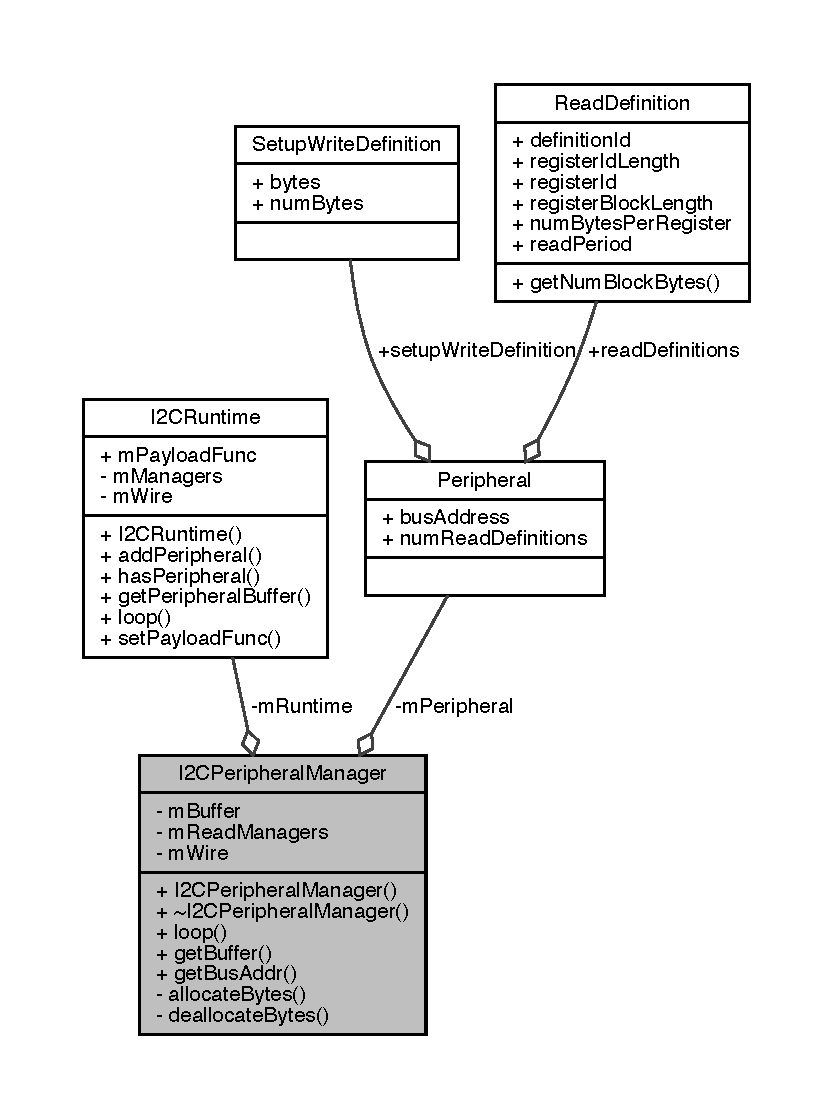
\includegraphics[width=350pt]{class_i2_c_peripheral_manager__coll__graph}
\end{center}
\end{figure}
\subsection*{Public Member Functions}
\begin{DoxyCompactItemize}
\item 
\mbox{\hyperlink{class_i2_c_peripheral_manager_a1e0399fb1723c895e13997275b686790}{I2\+C\+Peripheral\+Manager}} (\mbox{\hyperlink{struct_peripheral}{Peripheral}} $\ast$peripheral, Two\+Wire $\ast$\mbox{\hyperlink{main_8cpp_ab8d8f9af97a698a5a73132c347acbaf4}{wire}}, \mbox{\hyperlink{class_i2_c_runtime}{I2\+C\+Runtime}} $\ast$\mbox{\hyperlink{main_8cpp_a1fa047c23d7c85d1ad97022cd6b157d0}{runtime}})
\item 
\mbox{\hyperlink{class_i2_c_peripheral_manager_aee8ee79532efd6cfd2e684f0528bf1ba}{$\sim$\+I2\+C\+Peripheral\+Manager}} ()
\item 
void \mbox{\hyperlink{class_i2_c_peripheral_manager_a528b94dd1fbb9271a0e8bf7d4c4e53b6}{loop}} ()
\item 
uint8\+\_\+t $\ast$$\ast$ \mbox{\hyperlink{class_i2_c_peripheral_manager_a0405f2a121ad0c1c62a34104ebf8adff}{get\+Buffer}} ()
\item 
uint8\+\_\+t \mbox{\hyperlink{class_i2_c_peripheral_manager_ab0491e2a0f08b02533a96aae26003542}{get\+Bus\+Addr}} ()
\end{DoxyCompactItemize}
\subsection*{Static Private Member Functions}
\begin{DoxyCompactItemize}
\item 
static uint8\+\_\+t $\ast$$\ast$ \mbox{\hyperlink{class_i2_c_peripheral_manager_ac97eada0dc89503e0cc9ea56a6124ad0}{allocate\+Bytes}} (\mbox{\hyperlink{struct_peripheral}{Peripheral}} $\ast$)
\item 
static void \mbox{\hyperlink{class_i2_c_peripheral_manager_a4b1ea76c3c967214a21e1470c0176920}{deallocate\+Bytes}} (\mbox{\hyperlink{struct_peripheral}{Peripheral}} $\ast$, uint8\+\_\+t $\ast$$\ast$)
\end{DoxyCompactItemize}
\subsection*{Private Attributes}
\begin{DoxyCompactItemize}
\item 
\mbox{\hyperlink{struct_peripheral}{Peripheral}} $\ast$ \mbox{\hyperlink{class_i2_c_peripheral_manager_a758e4afa2027a73681b171219ba4cd50}{m\+Peripheral}}
\item 
uint8\+\_\+t $\ast$$\ast$ \mbox{\hyperlink{class_i2_c_peripheral_manager_a2460262d9bdd68a81f2dee42651a1ad8}{m\+Buffer}}
\item 
std\+::vector$<$ \mbox{\hyperlink{class_i2_c_read_manager}{I2\+C\+Read\+Manager}} $\ast$ $>$ \mbox{\hyperlink{class_i2_c_peripheral_manager_adf8ae8159cf193f1b004c6a2158ddf2d}{m\+Read\+Managers}}
\item 
Two\+Wire $\ast$ \mbox{\hyperlink{class_i2_c_peripheral_manager_a348d218edc48d69e21f8a0e204fde50a}{m\+Wire}}
\item 
\mbox{\hyperlink{class_i2_c_runtime}{I2\+C\+Runtime}} $\ast$ \mbox{\hyperlink{class_i2_c_peripheral_manager_a7dbb8937bebdd3e21d88728f02656422}{m\+Runtime}}
\end{DoxyCompactItemize}


\subsection{Detailed Description}
Manages all the read managers and memory allocation for a single peripheral. 

Only intended to be used by an \mbox{\hyperlink{class_i2_c_runtime}{I2\+C\+Runtime}} instance.

A peripheral manager will manage the read managers for each read definition on a single peripheral. 

\subsection{Constructor \& Destructor Documentation}
\mbox{\Hypertarget{class_i2_c_peripheral_manager_a1e0399fb1723c895e13997275b686790}\label{class_i2_c_peripheral_manager_a1e0399fb1723c895e13997275b686790}} 
\index{I2\+C\+Peripheral\+Manager@{I2\+C\+Peripheral\+Manager}!I2\+C\+Peripheral\+Manager@{I2\+C\+Peripheral\+Manager}}
\index{I2\+C\+Peripheral\+Manager@{I2\+C\+Peripheral\+Manager}!I2\+C\+Peripheral\+Manager@{I2\+C\+Peripheral\+Manager}}
\subsubsection{\texorpdfstring{I2\+C\+Peripheral\+Manager()}{I2CPeripheralManager()}}
{\footnotesize\ttfamily I2\+C\+Peripheral\+Manager\+::\+I2\+C\+Peripheral\+Manager (\begin{DoxyParamCaption}\item[{\mbox{\hyperlink{struct_peripheral}{Peripheral}} $\ast$}]{peripheral,  }\item[{Two\+Wire $\ast$}]{wire,  }\item[{\mbox{\hyperlink{class_i2_c_runtime}{I2\+C\+Runtime}} $\ast$}]{runtime }\end{DoxyParamCaption})}

\mbox{\Hypertarget{class_i2_c_peripheral_manager_aee8ee79532efd6cfd2e684f0528bf1ba}\label{class_i2_c_peripheral_manager_aee8ee79532efd6cfd2e684f0528bf1ba}} 
\index{I2\+C\+Peripheral\+Manager@{I2\+C\+Peripheral\+Manager}!````~I2\+C\+Peripheral\+Manager@{$\sim$\+I2\+C\+Peripheral\+Manager}}
\index{````~I2\+C\+Peripheral\+Manager@{$\sim$\+I2\+C\+Peripheral\+Manager}!I2\+C\+Peripheral\+Manager@{I2\+C\+Peripheral\+Manager}}
\subsubsection{\texorpdfstring{$\sim$\+I2\+C\+Peripheral\+Manager()}{~I2CPeripheralManager()}}
{\footnotesize\ttfamily I2\+C\+Peripheral\+Manager\+::$\sim$\+I2\+C\+Peripheral\+Manager (\begin{DoxyParamCaption}{ }\end{DoxyParamCaption})}



\subsection{Member Function Documentation}
\mbox{\Hypertarget{class_i2_c_peripheral_manager_ac97eada0dc89503e0cc9ea56a6124ad0}\label{class_i2_c_peripheral_manager_ac97eada0dc89503e0cc9ea56a6124ad0}} 
\index{I2\+C\+Peripheral\+Manager@{I2\+C\+Peripheral\+Manager}!allocate\+Bytes@{allocate\+Bytes}}
\index{allocate\+Bytes@{allocate\+Bytes}!I2\+C\+Peripheral\+Manager@{I2\+C\+Peripheral\+Manager}}
\subsubsection{\texorpdfstring{allocate\+Bytes()}{allocateBytes()}}
{\footnotesize\ttfamily uint8\+\_\+t $\ast$$\ast$ I2\+C\+Peripheral\+Manager\+::allocate\+Bytes (\begin{DoxyParamCaption}\item[{\mbox{\hyperlink{struct_peripheral}{Peripheral}} $\ast$}]{peripheral }\end{DoxyParamCaption})\hspace{0.3cm}{\ttfamily [static]}, {\ttfamily [private]}}

\mbox{\Hypertarget{class_i2_c_peripheral_manager_a4b1ea76c3c967214a21e1470c0176920}\label{class_i2_c_peripheral_manager_a4b1ea76c3c967214a21e1470c0176920}} 
\index{I2\+C\+Peripheral\+Manager@{I2\+C\+Peripheral\+Manager}!deallocate\+Bytes@{deallocate\+Bytes}}
\index{deallocate\+Bytes@{deallocate\+Bytes}!I2\+C\+Peripheral\+Manager@{I2\+C\+Peripheral\+Manager}}
\subsubsection{\texorpdfstring{deallocate\+Bytes()}{deallocateBytes()}}
{\footnotesize\ttfamily void I2\+C\+Peripheral\+Manager\+::deallocate\+Bytes (\begin{DoxyParamCaption}\item[{\mbox{\hyperlink{struct_peripheral}{Peripheral}} $\ast$}]{peripheral,  }\item[{uint8\+\_\+t $\ast$$\ast$}]{bytes }\end{DoxyParamCaption})\hspace{0.3cm}{\ttfamily [static]}, {\ttfamily [private]}}

\mbox{\Hypertarget{class_i2_c_peripheral_manager_a0405f2a121ad0c1c62a34104ebf8adff}\label{class_i2_c_peripheral_manager_a0405f2a121ad0c1c62a34104ebf8adff}} 
\index{I2\+C\+Peripheral\+Manager@{I2\+C\+Peripheral\+Manager}!get\+Buffer@{get\+Buffer}}
\index{get\+Buffer@{get\+Buffer}!I2\+C\+Peripheral\+Manager@{I2\+C\+Peripheral\+Manager}}
\subsubsection{\texorpdfstring{get\+Buffer()}{getBuffer()}}
{\footnotesize\ttfamily uint8\+\_\+t $\ast$$\ast$ I2\+C\+Peripheral\+Manager\+::get\+Buffer (\begin{DoxyParamCaption}{ }\end{DoxyParamCaption})}

\mbox{\Hypertarget{class_i2_c_peripheral_manager_ab0491e2a0f08b02533a96aae26003542}\label{class_i2_c_peripheral_manager_ab0491e2a0f08b02533a96aae26003542}} 
\index{I2\+C\+Peripheral\+Manager@{I2\+C\+Peripheral\+Manager}!get\+Bus\+Addr@{get\+Bus\+Addr}}
\index{get\+Bus\+Addr@{get\+Bus\+Addr}!I2\+C\+Peripheral\+Manager@{I2\+C\+Peripheral\+Manager}}
\subsubsection{\texorpdfstring{get\+Bus\+Addr()}{getBusAddr()}}
{\footnotesize\ttfamily uint8\+\_\+t I2\+C\+Peripheral\+Manager\+::get\+Bus\+Addr (\begin{DoxyParamCaption}{ }\end{DoxyParamCaption})}

\mbox{\Hypertarget{class_i2_c_peripheral_manager_a528b94dd1fbb9271a0e8bf7d4c4e53b6}\label{class_i2_c_peripheral_manager_a528b94dd1fbb9271a0e8bf7d4c4e53b6}} 
\index{I2\+C\+Peripheral\+Manager@{I2\+C\+Peripheral\+Manager}!loop@{loop}}
\index{loop@{loop}!I2\+C\+Peripheral\+Manager@{I2\+C\+Peripheral\+Manager}}
\subsubsection{\texorpdfstring{loop()}{loop()}}
{\footnotesize\ttfamily void I2\+C\+Peripheral\+Manager\+::loop (\begin{DoxyParamCaption}{ }\end{DoxyParamCaption})}



\subsection{Member Data Documentation}
\mbox{\Hypertarget{class_i2_c_peripheral_manager_a2460262d9bdd68a81f2dee42651a1ad8}\label{class_i2_c_peripheral_manager_a2460262d9bdd68a81f2dee42651a1ad8}} 
\index{I2\+C\+Peripheral\+Manager@{I2\+C\+Peripheral\+Manager}!m\+Buffer@{m\+Buffer}}
\index{m\+Buffer@{m\+Buffer}!I2\+C\+Peripheral\+Manager@{I2\+C\+Peripheral\+Manager}}
\subsubsection{\texorpdfstring{m\+Buffer}{mBuffer}}
{\footnotesize\ttfamily uint8\+\_\+t$\ast$$\ast$ I2\+C\+Peripheral\+Manager\+::m\+Buffer\hspace{0.3cm}{\ttfamily [private]}}

\mbox{\Hypertarget{class_i2_c_peripheral_manager_a758e4afa2027a73681b171219ba4cd50}\label{class_i2_c_peripheral_manager_a758e4afa2027a73681b171219ba4cd50}} 
\index{I2\+C\+Peripheral\+Manager@{I2\+C\+Peripheral\+Manager}!m\+Peripheral@{m\+Peripheral}}
\index{m\+Peripheral@{m\+Peripheral}!I2\+C\+Peripheral\+Manager@{I2\+C\+Peripheral\+Manager}}
\subsubsection{\texorpdfstring{m\+Peripheral}{mPeripheral}}
{\footnotesize\ttfamily \mbox{\hyperlink{struct_peripheral}{Peripheral}}$\ast$ I2\+C\+Peripheral\+Manager\+::m\+Peripheral\hspace{0.3cm}{\ttfamily [private]}}

\mbox{\Hypertarget{class_i2_c_peripheral_manager_adf8ae8159cf193f1b004c6a2158ddf2d}\label{class_i2_c_peripheral_manager_adf8ae8159cf193f1b004c6a2158ddf2d}} 
\index{I2\+C\+Peripheral\+Manager@{I2\+C\+Peripheral\+Manager}!m\+Read\+Managers@{m\+Read\+Managers}}
\index{m\+Read\+Managers@{m\+Read\+Managers}!I2\+C\+Peripheral\+Manager@{I2\+C\+Peripheral\+Manager}}
\subsubsection{\texorpdfstring{m\+Read\+Managers}{mReadManagers}}
{\footnotesize\ttfamily std\+::vector$<$\mbox{\hyperlink{class_i2_c_read_manager}{I2\+C\+Read\+Manager}} $\ast$$>$ I2\+C\+Peripheral\+Manager\+::m\+Read\+Managers\hspace{0.3cm}{\ttfamily [private]}}

\mbox{\Hypertarget{class_i2_c_peripheral_manager_a7dbb8937bebdd3e21d88728f02656422}\label{class_i2_c_peripheral_manager_a7dbb8937bebdd3e21d88728f02656422}} 
\index{I2\+C\+Peripheral\+Manager@{I2\+C\+Peripheral\+Manager}!m\+Runtime@{m\+Runtime}}
\index{m\+Runtime@{m\+Runtime}!I2\+C\+Peripheral\+Manager@{I2\+C\+Peripheral\+Manager}}
\subsubsection{\texorpdfstring{m\+Runtime}{mRuntime}}
{\footnotesize\ttfamily \mbox{\hyperlink{class_i2_c_runtime}{I2\+C\+Runtime}}$\ast$ I2\+C\+Peripheral\+Manager\+::m\+Runtime\hspace{0.3cm}{\ttfamily [private]}}

\mbox{\Hypertarget{class_i2_c_peripheral_manager_a348d218edc48d69e21f8a0e204fde50a}\label{class_i2_c_peripheral_manager_a348d218edc48d69e21f8a0e204fde50a}} 
\index{I2\+C\+Peripheral\+Manager@{I2\+C\+Peripheral\+Manager}!m\+Wire@{m\+Wire}}
\index{m\+Wire@{m\+Wire}!I2\+C\+Peripheral\+Manager@{I2\+C\+Peripheral\+Manager}}
\subsubsection{\texorpdfstring{m\+Wire}{mWire}}
{\footnotesize\ttfamily Two\+Wire$\ast$ I2\+C\+Peripheral\+Manager\+::m\+Wire\hspace{0.3cm}{\ttfamily [private]}}



The documentation for this class was generated from the following files\+:\begin{DoxyCompactItemize}
\item 
include/\mbox{\hyperlink{_i2_c_runtime_8h}{I2\+C\+Runtime.\+h}}\item 
src/\mbox{\hyperlink{_i2_c_runtime_8cpp}{I2\+C\+Runtime.\+cpp}}\end{DoxyCompactItemize}

\hypertarget{class_i2_c_read_manager}{}\section{I2\+C\+Read\+Manager Class Reference}
\label{class_i2_c_read_manager}\index{I2\+C\+Read\+Manager@{I2\+C\+Read\+Manager}}


Responsible for a state machine which reads data from the I2C bus in a non-\/blocking fashion.  




{\ttfamily \#include $<$I2\+C\+Read\+Manager.\+h$>$}



Collaboration diagram for I2\+C\+Read\+Manager\+:\nopagebreak
\begin{figure}[H]
\begin{center}
\leavevmode
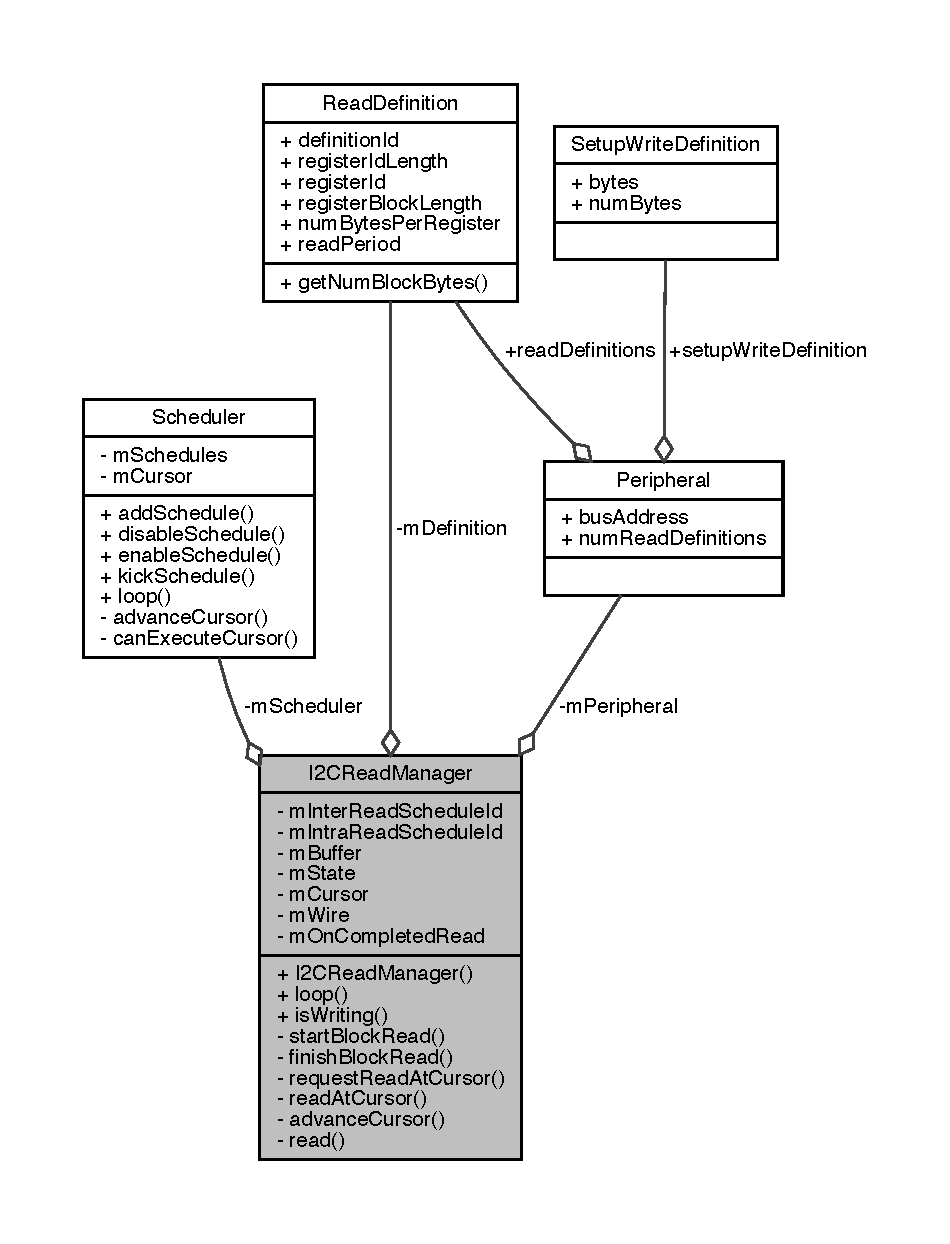
\includegraphics[width=350pt]{class_i2_c_read_manager__coll__graph}
\end{center}
\end{figure}
\subsection*{Public Member Functions}
\begin{DoxyCompactItemize}
\item 
\mbox{\hyperlink{class_i2_c_read_manager_a32c36b6f8c14cc7c8d845b2c9e4e3884}{I2\+C\+Read\+Manager}} (\mbox{\hyperlink{struct_read_definition}{Read\+Definition}} $\ast$, \mbox{\hyperlink{struct_peripheral}{Peripheral}} $\ast$, uint8\+\_\+t $\ast$, Two\+Wire $\ast$, std\+::shared\+\_\+ptr$<$ \mbox{\hyperlink{_scheduler_8h_a2125a5a2949d6ee13163b671159c0d4d}{Func}} $>$)
\item 
void \mbox{\hyperlink{class_i2_c_read_manager_a5ce39fa21f4cba4e6ea32899991d327e}{loop}} ()
\item 
bool \mbox{\hyperlink{class_i2_c_read_manager_a570077135c889571f51a1b68b30faaad}{is\+Writing}} ()
\end{DoxyCompactItemize}
\subsection*{Private Member Functions}
\begin{DoxyCompactItemize}
\item 
void \mbox{\hyperlink{class_i2_c_read_manager_a478faffbf411c694c81668c9687177bd}{start\+Block\+Read}} ()
\item 
void \mbox{\hyperlink{class_i2_c_read_manager_ab56d84786e053cd555e11c67eeed1d27}{finish\+Block\+Read}} ()
\item 
void \mbox{\hyperlink{class_i2_c_read_manager_a069f4a54d98b35f365b04f7272b30cd3}{request\+Read\+At\+Cursor}} ()
\item 
void \mbox{\hyperlink{class_i2_c_read_manager_ad9b045650b074a8b10ea472dec42cf71}{read\+At\+Cursor}} ()
\item 
void \mbox{\hyperlink{class_i2_c_read_manager_a3b901ae787a7e5c94004ed70fea67c49}{advance\+Cursor}} ()
\item 
void \mbox{\hyperlink{class_i2_c_read_manager_a7d4d8b3241291a25c7e82821d33df4db}{read}} ()
\end{DoxyCompactItemize}
\subsection*{Private Attributes}
\begin{DoxyCompactItemize}
\item 
\mbox{\hyperlink{struct_read_definition}{Read\+Definition}} $\ast$ \mbox{\hyperlink{class_i2_c_read_manager_a9a3f55a2c1fed16d7e17b16c153f0b32}{m\+Definition}}
\item 
\mbox{\hyperlink{struct_peripheral}{Peripheral}} $\ast$ \mbox{\hyperlink{class_i2_c_read_manager_a013d5feaf3f4d648b7ee840bd600aaf6}{m\+Peripheral}}
\item 
\mbox{\hyperlink{class_scheduler}{Scheduler}} \mbox{\hyperlink{class_i2_c_read_manager_a948854518d1720e57ce3980308e47f23}{m\+Scheduler}}
\item 
\mbox{\hyperlink{_scheduler_8h_a1e3b4605bdcbb8f6df7c47013e26e910}{Schedule\+Id}} \mbox{\hyperlink{class_i2_c_read_manager_abdf4bf35894f1b91f8af92b2de6ef709}{m\+Inter\+Read\+Schedule\+Id}}
\item 
\mbox{\hyperlink{_scheduler_8h_a1e3b4605bdcbb8f6df7c47013e26e910}{Schedule\+Id}} \mbox{\hyperlink{class_i2_c_read_manager_ad8505529aa2361af0e89087f679b0f80}{m\+Intra\+Read\+Schedule\+Id}}
\item 
uint8\+\_\+t $\ast$ \mbox{\hyperlink{class_i2_c_read_manager_af4df317c2ac86fa929f85c96b5d9a56b}{m\+Buffer}}
\item 
\mbox{\hyperlink{_i2_c_read_manager_8h_a6fa8ade9cf010a4fd9f7a36c4a4566aa}{Read\+Manager\+State}} \mbox{\hyperlink{class_i2_c_read_manager_ad3377b1f52aceee0bd2aa4597521b20a}{m\+State}}
\item 
uint16\+\_\+t \mbox{\hyperlink{class_i2_c_read_manager_a38cc98d6047836aec409733a8591ce2e}{m\+Cursor}}
\item 
Two\+Wire $\ast$ \mbox{\hyperlink{class_i2_c_read_manager_ab030eaa59d0661eb7b980a0419236788}{m\+Wire}}
\item 
std\+::shared\+\_\+ptr$<$ \mbox{\hyperlink{_scheduler_8h_a2125a5a2949d6ee13163b671159c0d4d}{Func}} $>$ \mbox{\hyperlink{class_i2_c_read_manager_a60fc6315a6e4bb48341c095907a36941}{m\+On\+Completed\+Read}}
\end{DoxyCompactItemize}


\subsection{Detailed Description}
Responsible for a state machine which reads data from the I2C bus in a non-\/blocking fashion. 

\subsection{Constructor \& Destructor Documentation}
\mbox{\Hypertarget{class_i2_c_read_manager_a32c36b6f8c14cc7c8d845b2c9e4e3884}\label{class_i2_c_read_manager_a32c36b6f8c14cc7c8d845b2c9e4e3884}} 
\index{I2\+C\+Read\+Manager@{I2\+C\+Read\+Manager}!I2\+C\+Read\+Manager@{I2\+C\+Read\+Manager}}
\index{I2\+C\+Read\+Manager@{I2\+C\+Read\+Manager}!I2\+C\+Read\+Manager@{I2\+C\+Read\+Manager}}
\subsubsection{\texorpdfstring{I2\+C\+Read\+Manager()}{I2CReadManager()}}
{\footnotesize\ttfamily I2\+C\+Read\+Manager\+::\+I2\+C\+Read\+Manager (\begin{DoxyParamCaption}\item[{\mbox{\hyperlink{struct_read_definition}{Read\+Definition}} $\ast$}]{read\+Definition,  }\item[{\mbox{\hyperlink{struct_peripheral}{Peripheral}} $\ast$}]{peripheral,  }\item[{uint8\+\_\+t $\ast$}]{buffer,  }\item[{Two\+Wire $\ast$}]{wire,  }\item[{std\+::shared\+\_\+ptr$<$ \mbox{\hyperlink{_scheduler_8h_a2125a5a2949d6ee13163b671159c0d4d}{Func}} $>$}]{on\+Completed\+Read\+Callback }\end{DoxyParamCaption})}



\subsection{Member Function Documentation}
\mbox{\Hypertarget{class_i2_c_read_manager_a3b901ae787a7e5c94004ed70fea67c49}\label{class_i2_c_read_manager_a3b901ae787a7e5c94004ed70fea67c49}} 
\index{I2\+C\+Read\+Manager@{I2\+C\+Read\+Manager}!advance\+Cursor@{advance\+Cursor}}
\index{advance\+Cursor@{advance\+Cursor}!I2\+C\+Read\+Manager@{I2\+C\+Read\+Manager}}
\subsubsection{\texorpdfstring{advance\+Cursor()}{advanceCursor()}}
{\footnotesize\ttfamily void I2\+C\+Read\+Manager\+::advance\+Cursor (\begin{DoxyParamCaption}{ }\end{DoxyParamCaption})\hspace{0.3cm}{\ttfamily [private]}}

\mbox{\Hypertarget{class_i2_c_read_manager_ab56d84786e053cd555e11c67eeed1d27}\label{class_i2_c_read_manager_ab56d84786e053cd555e11c67eeed1d27}} 
\index{I2\+C\+Read\+Manager@{I2\+C\+Read\+Manager}!finish\+Block\+Read@{finish\+Block\+Read}}
\index{finish\+Block\+Read@{finish\+Block\+Read}!I2\+C\+Read\+Manager@{I2\+C\+Read\+Manager}}
\subsubsection{\texorpdfstring{finish\+Block\+Read()}{finishBlockRead()}}
{\footnotesize\ttfamily void I2\+C\+Read\+Manager\+::finish\+Block\+Read (\begin{DoxyParamCaption}{ }\end{DoxyParamCaption})\hspace{0.3cm}{\ttfamily [private]}}

We\textquotesingle{}ve finished reading a from a contiguous block of register I\+Ds and can disable the intra-\/read schedule and switch back to the inter-\/read schedule. \mbox{\Hypertarget{class_i2_c_read_manager_a570077135c889571f51a1b68b30faaad}\label{class_i2_c_read_manager_a570077135c889571f51a1b68b30faaad}} 
\index{I2\+C\+Read\+Manager@{I2\+C\+Read\+Manager}!is\+Writing@{is\+Writing}}
\index{is\+Writing@{is\+Writing}!I2\+C\+Read\+Manager@{I2\+C\+Read\+Manager}}
\subsubsection{\texorpdfstring{is\+Writing()}{isWriting()}}
{\footnotesize\ttfamily bool I2\+C\+Read\+Manager\+::is\+Writing (\begin{DoxyParamCaption}{ }\end{DoxyParamCaption})}

\mbox{\Hypertarget{class_i2_c_read_manager_a5ce39fa21f4cba4e6ea32899991d327e}\label{class_i2_c_read_manager_a5ce39fa21f4cba4e6ea32899991d327e}} 
\index{I2\+C\+Read\+Manager@{I2\+C\+Read\+Manager}!loop@{loop}}
\index{loop@{loop}!I2\+C\+Read\+Manager@{I2\+C\+Read\+Manager}}
\subsubsection{\texorpdfstring{loop()}{loop()}}
{\footnotesize\ttfamily void I2\+C\+Read\+Manager\+::loop (\begin{DoxyParamCaption}{ }\end{DoxyParamCaption})}

\mbox{\Hypertarget{class_i2_c_read_manager_a7d4d8b3241291a25c7e82821d33df4db}\label{class_i2_c_read_manager_a7d4d8b3241291a25c7e82821d33df4db}} 
\index{I2\+C\+Read\+Manager@{I2\+C\+Read\+Manager}!read@{read}}
\index{read@{read}!I2\+C\+Read\+Manager@{I2\+C\+Read\+Manager}}
\subsubsection{\texorpdfstring{read()}{read()}}
{\footnotesize\ttfamily void I2\+C\+Read\+Manager\+::read (\begin{DoxyParamCaption}{ }\end{DoxyParamCaption})\hspace{0.3cm}{\ttfamily [private]}}

\mbox{\Hypertarget{class_i2_c_read_manager_ad9b045650b074a8b10ea472dec42cf71}\label{class_i2_c_read_manager_ad9b045650b074a8b10ea472dec42cf71}} 
\index{I2\+C\+Read\+Manager@{I2\+C\+Read\+Manager}!read\+At\+Cursor@{read\+At\+Cursor}}
\index{read\+At\+Cursor@{read\+At\+Cursor}!I2\+C\+Read\+Manager@{I2\+C\+Read\+Manager}}
\subsubsection{\texorpdfstring{read\+At\+Cursor()}{readAtCursor()}}
{\footnotesize\ttfamily void I2\+C\+Read\+Manager\+::read\+At\+Cursor (\begin{DoxyParamCaption}{ }\end{DoxyParamCaption})\hspace{0.3cm}{\ttfamily [private]}}

\mbox{\Hypertarget{class_i2_c_read_manager_a069f4a54d98b35f365b04f7272b30cd3}\label{class_i2_c_read_manager_a069f4a54d98b35f365b04f7272b30cd3}} 
\index{I2\+C\+Read\+Manager@{I2\+C\+Read\+Manager}!request\+Read\+At\+Cursor@{request\+Read\+At\+Cursor}}
\index{request\+Read\+At\+Cursor@{request\+Read\+At\+Cursor}!I2\+C\+Read\+Manager@{I2\+C\+Read\+Manager}}
\subsubsection{\texorpdfstring{request\+Read\+At\+Cursor()}{requestReadAtCursor()}}
{\footnotesize\ttfamily void I2\+C\+Read\+Manager\+::request\+Read\+At\+Cursor (\begin{DoxyParamCaption}{ }\end{DoxyParamCaption})\hspace{0.3cm}{\ttfamily [private]}}

\mbox{\Hypertarget{class_i2_c_read_manager_a478faffbf411c694c81668c9687177bd}\label{class_i2_c_read_manager_a478faffbf411c694c81668c9687177bd}} 
\index{I2\+C\+Read\+Manager@{I2\+C\+Read\+Manager}!start\+Block\+Read@{start\+Block\+Read}}
\index{start\+Block\+Read@{start\+Block\+Read}!I2\+C\+Read\+Manager@{I2\+C\+Read\+Manager}}
\subsubsection{\texorpdfstring{start\+Block\+Read()}{startBlockRead()}}
{\footnotesize\ttfamily void I2\+C\+Read\+Manager\+::start\+Block\+Read (\begin{DoxyParamCaption}{ }\end{DoxyParamCaption})\hspace{0.3cm}{\ttfamily [private]}}



\subsection{Member Data Documentation}
\mbox{\Hypertarget{class_i2_c_read_manager_af4df317c2ac86fa929f85c96b5d9a56b}\label{class_i2_c_read_manager_af4df317c2ac86fa929f85c96b5d9a56b}} 
\index{I2\+C\+Read\+Manager@{I2\+C\+Read\+Manager}!m\+Buffer@{m\+Buffer}}
\index{m\+Buffer@{m\+Buffer}!I2\+C\+Read\+Manager@{I2\+C\+Read\+Manager}}
\subsubsection{\texorpdfstring{m\+Buffer}{mBuffer}}
{\footnotesize\ttfamily uint8\+\_\+t$\ast$ I2\+C\+Read\+Manager\+::m\+Buffer\hspace{0.3cm}{\ttfamily [private]}}

The buffer for the whole peripheral is a 2D array that manages bytes per read definition. A single Read\+Manager instance only manages a single Rea\+Definition. This is the buffer for the single instance. \mbox{\Hypertarget{class_i2_c_read_manager_a38cc98d6047836aec409733a8591ce2e}\label{class_i2_c_read_manager_a38cc98d6047836aec409733a8591ce2e}} 
\index{I2\+C\+Read\+Manager@{I2\+C\+Read\+Manager}!m\+Cursor@{m\+Cursor}}
\index{m\+Cursor@{m\+Cursor}!I2\+C\+Read\+Manager@{I2\+C\+Read\+Manager}}
\subsubsection{\texorpdfstring{m\+Cursor}{mCursor}}
{\footnotesize\ttfamily uint16\+\_\+t I2\+C\+Read\+Manager\+::m\+Cursor\hspace{0.3cm}{\ttfamily [private]}}

\mbox{\Hypertarget{class_i2_c_read_manager_a9a3f55a2c1fed16d7e17b16c153f0b32}\label{class_i2_c_read_manager_a9a3f55a2c1fed16d7e17b16c153f0b32}} 
\index{I2\+C\+Read\+Manager@{I2\+C\+Read\+Manager}!m\+Definition@{m\+Definition}}
\index{m\+Definition@{m\+Definition}!I2\+C\+Read\+Manager@{I2\+C\+Read\+Manager}}
\subsubsection{\texorpdfstring{m\+Definition}{mDefinition}}
{\footnotesize\ttfamily \mbox{\hyperlink{struct_read_definition}{Read\+Definition}}$\ast$ I2\+C\+Read\+Manager\+::m\+Definition\hspace{0.3cm}{\ttfamily [private]}}

\mbox{\Hypertarget{class_i2_c_read_manager_abdf4bf35894f1b91f8af92b2de6ef709}\label{class_i2_c_read_manager_abdf4bf35894f1b91f8af92b2de6ef709}} 
\index{I2\+C\+Read\+Manager@{I2\+C\+Read\+Manager}!m\+Inter\+Read\+Schedule\+Id@{m\+Inter\+Read\+Schedule\+Id}}
\index{m\+Inter\+Read\+Schedule\+Id@{m\+Inter\+Read\+Schedule\+Id}!I2\+C\+Read\+Manager@{I2\+C\+Read\+Manager}}
\subsubsection{\texorpdfstring{m\+Inter\+Read\+Schedule\+Id}{mInterReadScheduleId}}
{\footnotesize\ttfamily \mbox{\hyperlink{_scheduler_8h_a1e3b4605bdcbb8f6df7c47013e26e910}{Schedule\+Id}} I2\+C\+Read\+Manager\+::m\+Inter\+Read\+Schedule\+Id\hspace{0.3cm}{\ttfamily [private]}}

\mbox{\Hypertarget{class_i2_c_read_manager_ad8505529aa2361af0e89087f679b0f80}\label{class_i2_c_read_manager_ad8505529aa2361af0e89087f679b0f80}} 
\index{I2\+C\+Read\+Manager@{I2\+C\+Read\+Manager}!m\+Intra\+Read\+Schedule\+Id@{m\+Intra\+Read\+Schedule\+Id}}
\index{m\+Intra\+Read\+Schedule\+Id@{m\+Intra\+Read\+Schedule\+Id}!I2\+C\+Read\+Manager@{I2\+C\+Read\+Manager}}
\subsubsection{\texorpdfstring{m\+Intra\+Read\+Schedule\+Id}{mIntraReadScheduleId}}
{\footnotesize\ttfamily \mbox{\hyperlink{_scheduler_8h_a1e3b4605bdcbb8f6df7c47013e26e910}{Schedule\+Id}} I2\+C\+Read\+Manager\+::m\+Intra\+Read\+Schedule\+Id\hspace{0.3cm}{\ttfamily [private]}}

\mbox{\Hypertarget{class_i2_c_read_manager_a60fc6315a6e4bb48341c095907a36941}\label{class_i2_c_read_manager_a60fc6315a6e4bb48341c095907a36941}} 
\index{I2\+C\+Read\+Manager@{I2\+C\+Read\+Manager}!m\+On\+Completed\+Read@{m\+On\+Completed\+Read}}
\index{m\+On\+Completed\+Read@{m\+On\+Completed\+Read}!I2\+C\+Read\+Manager@{I2\+C\+Read\+Manager}}
\subsubsection{\texorpdfstring{m\+On\+Completed\+Read}{mOnCompletedRead}}
{\footnotesize\ttfamily std\+::shared\+\_\+ptr$<$\mbox{\hyperlink{_scheduler_8h_a2125a5a2949d6ee13163b671159c0d4d}{Func}}$>$ I2\+C\+Read\+Manager\+::m\+On\+Completed\+Read\hspace{0.3cm}{\ttfamily [private]}}

\mbox{\Hypertarget{class_i2_c_read_manager_a013d5feaf3f4d648b7ee840bd600aaf6}\label{class_i2_c_read_manager_a013d5feaf3f4d648b7ee840bd600aaf6}} 
\index{I2\+C\+Read\+Manager@{I2\+C\+Read\+Manager}!m\+Peripheral@{m\+Peripheral}}
\index{m\+Peripheral@{m\+Peripheral}!I2\+C\+Read\+Manager@{I2\+C\+Read\+Manager}}
\subsubsection{\texorpdfstring{m\+Peripheral}{mPeripheral}}
{\footnotesize\ttfamily \mbox{\hyperlink{struct_peripheral}{Peripheral}}$\ast$ I2\+C\+Read\+Manager\+::m\+Peripheral\hspace{0.3cm}{\ttfamily [private]}}

\mbox{\Hypertarget{class_i2_c_read_manager_a948854518d1720e57ce3980308e47f23}\label{class_i2_c_read_manager_a948854518d1720e57ce3980308e47f23}} 
\index{I2\+C\+Read\+Manager@{I2\+C\+Read\+Manager}!m\+Scheduler@{m\+Scheduler}}
\index{m\+Scheduler@{m\+Scheduler}!I2\+C\+Read\+Manager@{I2\+C\+Read\+Manager}}
\subsubsection{\texorpdfstring{m\+Scheduler}{mScheduler}}
{\footnotesize\ttfamily \mbox{\hyperlink{class_scheduler}{Scheduler}} I2\+C\+Read\+Manager\+::m\+Scheduler\hspace{0.3cm}{\ttfamily [private]}}

\mbox{\Hypertarget{class_i2_c_read_manager_ad3377b1f52aceee0bd2aa4597521b20a}\label{class_i2_c_read_manager_ad3377b1f52aceee0bd2aa4597521b20a}} 
\index{I2\+C\+Read\+Manager@{I2\+C\+Read\+Manager}!m\+State@{m\+State}}
\index{m\+State@{m\+State}!I2\+C\+Read\+Manager@{I2\+C\+Read\+Manager}}
\subsubsection{\texorpdfstring{m\+State}{mState}}
{\footnotesize\ttfamily \mbox{\hyperlink{_i2_c_read_manager_8h_a6fa8ade9cf010a4fd9f7a36c4a4566aa}{Read\+Manager\+State}} I2\+C\+Read\+Manager\+::m\+State\hspace{0.3cm}{\ttfamily [private]}}

\mbox{\Hypertarget{class_i2_c_read_manager_ab030eaa59d0661eb7b980a0419236788}\label{class_i2_c_read_manager_ab030eaa59d0661eb7b980a0419236788}} 
\index{I2\+C\+Read\+Manager@{I2\+C\+Read\+Manager}!m\+Wire@{m\+Wire}}
\index{m\+Wire@{m\+Wire}!I2\+C\+Read\+Manager@{I2\+C\+Read\+Manager}}
\subsubsection{\texorpdfstring{m\+Wire}{mWire}}
{\footnotesize\ttfamily Two\+Wire$\ast$ I2\+C\+Read\+Manager\+::m\+Wire\hspace{0.3cm}{\ttfamily [private]}}



The documentation for this class was generated from the following files\+:\begin{DoxyCompactItemize}
\item 
include/\mbox{\hyperlink{_i2_c_read_manager_8h}{I2\+C\+Read\+Manager.\+h}}\item 
src/\mbox{\hyperlink{_i2_c_read_manager_8cpp}{I2\+C\+Read\+Manager.\+cpp}}\end{DoxyCompactItemize}

\hypertarget{class_i2_c_runtime}{}\section{I2\+C\+Runtime Class Reference}
\label{class_i2_c_runtime}\index{I2\+C\+Runtime@{I2\+C\+Runtime}}


Responsible for the primary event loop for all peripherals on the bus.  




{\ttfamily \#include $<$I2\+C\+Runtime.\+h$>$}



Collaboration diagram for I2\+C\+Runtime\+:\nopagebreak
\begin{figure}[H]
\begin{center}
\leavevmode
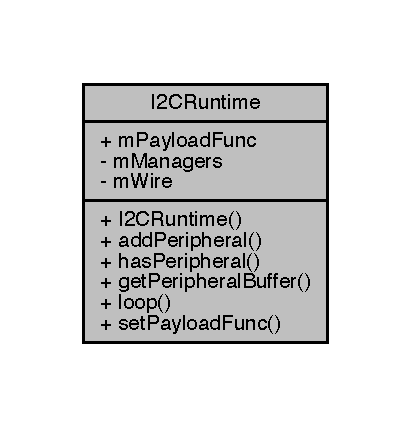
\includegraphics[width=197pt]{class_i2_c_runtime__coll__graph}
\end{center}
\end{figure}
\subsection*{Public Member Functions}
\begin{DoxyCompactItemize}
\item 
\mbox{\hyperlink{class_i2_c_runtime_aa68ca8901478720ad84ec7fb5f7f1494}{I2\+C\+Runtime}} (Two\+Wire $\ast$)
\item 
std\+::size\+\_\+t \mbox{\hyperlink{class_i2_c_runtime_aba281d78dfd704b614f0e126e9f846e5}{add\+Peripheral}} (\mbox{\hyperlink{struct_peripheral}{Peripheral}} $\ast$peripheral)
\item 
bool \mbox{\hyperlink{class_i2_c_runtime_a945f727b6d885e2c191d547b9f66f679}{has\+Peripheral}} (std\+::size\+\_\+t)
\item 
uint8\+\_\+t $\ast$$\ast$ \mbox{\hyperlink{class_i2_c_runtime_a68052a5397fdb5a1cd408d2e6ff0bac2}{get\+Peripheral\+Buffer}} (std\+::size\+\_\+t)
\item 
void \mbox{\hyperlink{class_i2_c_runtime_a7fd85af000f8d514f94c2f92db1ddfaa}{loop}} ()
\item 
void \mbox{\hyperlink{class_i2_c_runtime_a1ce8a62c677e64e8113376fc1264c6e6}{set\+Payload\+Func}} (std\+::shared\+\_\+ptr$<$ \mbox{\hyperlink{_telemetry_protocol_8h_a98c05796bd59110e8ae10dc71580b759}{Payload\+Func}} $>$)
\end{DoxyCompactItemize}
\subsection*{Public Attributes}
\begin{DoxyCompactItemize}
\item 
std\+::shared\+\_\+ptr$<$ \mbox{\hyperlink{_telemetry_protocol_8h_a98c05796bd59110e8ae10dc71580b759}{Payload\+Func}} $>$ \mbox{\hyperlink{class_i2_c_runtime_a2e84a62078fc0169f8abd9e126ed5f38}{m\+Payload\+Func}}
\end{DoxyCompactItemize}
\subsection*{Private Attributes}
\begin{DoxyCompactItemize}
\item 
std\+::vector$<$ \mbox{\hyperlink{class_i2_c_peripheral_manager}{I2\+C\+Peripheral\+Manager}} $\ast$ $>$ \mbox{\hyperlink{class_i2_c_runtime_a399a771421014539f95a53e58debc341}{m\+Managers}}
\item 
Two\+Wire $\ast$ \mbox{\hyperlink{class_i2_c_runtime_a89c15b30195945ec61834ee3f7f8ac88}{m\+Wire}}
\end{DoxyCompactItemize}


\subsection{Detailed Description}
Responsible for the primary event loop for all peripherals on the bus. 

\subsection{Constructor \& Destructor Documentation}
\mbox{\Hypertarget{class_i2_c_runtime_aa68ca8901478720ad84ec7fb5f7f1494}\label{class_i2_c_runtime_aa68ca8901478720ad84ec7fb5f7f1494}} 
\index{I2\+C\+Runtime@{I2\+C\+Runtime}!I2\+C\+Runtime@{I2\+C\+Runtime}}
\index{I2\+C\+Runtime@{I2\+C\+Runtime}!I2\+C\+Runtime@{I2\+C\+Runtime}}
\subsubsection{\texorpdfstring{I2\+C\+Runtime()}{I2CRuntime()}}
{\footnotesize\ttfamily I2\+C\+Runtime\+::\+I2\+C\+Runtime (\begin{DoxyParamCaption}\item[{Two\+Wire $\ast$}]{wire }\end{DoxyParamCaption})}



\subsection{Member Function Documentation}
\mbox{\Hypertarget{class_i2_c_runtime_aba281d78dfd704b614f0e126e9f846e5}\label{class_i2_c_runtime_aba281d78dfd704b614f0e126e9f846e5}} 
\index{I2\+C\+Runtime@{I2\+C\+Runtime}!add\+Peripheral@{add\+Peripheral}}
\index{add\+Peripheral@{add\+Peripheral}!I2\+C\+Runtime@{I2\+C\+Runtime}}
\subsubsection{\texorpdfstring{add\+Peripheral()}{addPeripheral()}}
{\footnotesize\ttfamily std\+::size\+\_\+t I2\+C\+Runtime\+::add\+Peripheral (\begin{DoxyParamCaption}\item[{\mbox{\hyperlink{struct_peripheral}{Peripheral}} $\ast$}]{peripheral }\end{DoxyParamCaption})}

\mbox{\Hypertarget{class_i2_c_runtime_a68052a5397fdb5a1cd408d2e6ff0bac2}\label{class_i2_c_runtime_a68052a5397fdb5a1cd408d2e6ff0bac2}} 
\index{I2\+C\+Runtime@{I2\+C\+Runtime}!get\+Peripheral\+Buffer@{get\+Peripheral\+Buffer}}
\index{get\+Peripheral\+Buffer@{get\+Peripheral\+Buffer}!I2\+C\+Runtime@{I2\+C\+Runtime}}
\subsubsection{\texorpdfstring{get\+Peripheral\+Buffer()}{getPeripheralBuffer()}}
{\footnotesize\ttfamily uint8\+\_\+t $\ast$$\ast$ I2\+C\+Runtime\+::get\+Peripheral\+Buffer (\begin{DoxyParamCaption}\item[{std\+::size\+\_\+t}]{peripheral\+Id }\end{DoxyParamCaption})}

\mbox{\Hypertarget{class_i2_c_runtime_a945f727b6d885e2c191d547b9f66f679}\label{class_i2_c_runtime_a945f727b6d885e2c191d547b9f66f679}} 
\index{I2\+C\+Runtime@{I2\+C\+Runtime}!has\+Peripheral@{has\+Peripheral}}
\index{has\+Peripheral@{has\+Peripheral}!I2\+C\+Runtime@{I2\+C\+Runtime}}
\subsubsection{\texorpdfstring{has\+Peripheral()}{hasPeripheral()}}
{\footnotesize\ttfamily bool I2\+C\+Runtime\+::has\+Peripheral (\begin{DoxyParamCaption}\item[{std\+::size\+\_\+t}]{peripheral\+Id }\end{DoxyParamCaption})}

\mbox{\Hypertarget{class_i2_c_runtime_a7fd85af000f8d514f94c2f92db1ddfaa}\label{class_i2_c_runtime_a7fd85af000f8d514f94c2f92db1ddfaa}} 
\index{I2\+C\+Runtime@{I2\+C\+Runtime}!loop@{loop}}
\index{loop@{loop}!I2\+C\+Runtime@{I2\+C\+Runtime}}
\subsubsection{\texorpdfstring{loop()}{loop()}}
{\footnotesize\ttfamily void I2\+C\+Runtime\+::loop (\begin{DoxyParamCaption}{ }\end{DoxyParamCaption})}

\mbox{\Hypertarget{class_i2_c_runtime_a1ce8a62c677e64e8113376fc1264c6e6}\label{class_i2_c_runtime_a1ce8a62c677e64e8113376fc1264c6e6}} 
\index{I2\+C\+Runtime@{I2\+C\+Runtime}!set\+Payload\+Func@{set\+Payload\+Func}}
\index{set\+Payload\+Func@{set\+Payload\+Func}!I2\+C\+Runtime@{I2\+C\+Runtime}}
\subsubsection{\texorpdfstring{set\+Payload\+Func()}{setPayloadFunc()}}
{\footnotesize\ttfamily void I2\+C\+Runtime\+::set\+Payload\+Func (\begin{DoxyParamCaption}\item[{std\+::shared\+\_\+ptr$<$ \mbox{\hyperlink{_telemetry_protocol_8h_a98c05796bd59110e8ae10dc71580b759}{Payload\+Func}} $>$}]{func }\end{DoxyParamCaption})}



\subsection{Member Data Documentation}
\mbox{\Hypertarget{class_i2_c_runtime_a399a771421014539f95a53e58debc341}\label{class_i2_c_runtime_a399a771421014539f95a53e58debc341}} 
\index{I2\+C\+Runtime@{I2\+C\+Runtime}!m\+Managers@{m\+Managers}}
\index{m\+Managers@{m\+Managers}!I2\+C\+Runtime@{I2\+C\+Runtime}}
\subsubsection{\texorpdfstring{m\+Managers}{mManagers}}
{\footnotesize\ttfamily std\+::vector$<$\mbox{\hyperlink{class_i2_c_peripheral_manager}{I2\+C\+Peripheral\+Manager}} $\ast$$>$ I2\+C\+Runtime\+::m\+Managers\hspace{0.3cm}{\ttfamily [private]}}

\mbox{\Hypertarget{class_i2_c_runtime_a2e84a62078fc0169f8abd9e126ed5f38}\label{class_i2_c_runtime_a2e84a62078fc0169f8abd9e126ed5f38}} 
\index{I2\+C\+Runtime@{I2\+C\+Runtime}!m\+Payload\+Func@{m\+Payload\+Func}}
\index{m\+Payload\+Func@{m\+Payload\+Func}!I2\+C\+Runtime@{I2\+C\+Runtime}}
\subsubsection{\texorpdfstring{m\+Payload\+Func}{mPayloadFunc}}
{\footnotesize\ttfamily std\+::shared\+\_\+ptr$<$\mbox{\hyperlink{_telemetry_protocol_8h_a98c05796bd59110e8ae10dc71580b759}{Payload\+Func}}$>$ I2\+C\+Runtime\+::m\+Payload\+Func}

\mbox{\Hypertarget{class_i2_c_runtime_a89c15b30195945ec61834ee3f7f8ac88}\label{class_i2_c_runtime_a89c15b30195945ec61834ee3f7f8ac88}} 
\index{I2\+C\+Runtime@{I2\+C\+Runtime}!m\+Wire@{m\+Wire}}
\index{m\+Wire@{m\+Wire}!I2\+C\+Runtime@{I2\+C\+Runtime}}
\subsubsection{\texorpdfstring{m\+Wire}{mWire}}
{\footnotesize\ttfamily Two\+Wire$\ast$ I2\+C\+Runtime\+::m\+Wire\hspace{0.3cm}{\ttfamily [private]}}



The documentation for this class was generated from the following files\+:\begin{DoxyCompactItemize}
\item 
include/\mbox{\hyperlink{_i2_c_runtime_8h}{I2\+C\+Runtime.\+h}}\item 
src/\mbox{\hyperlink{_i2_c_runtime_8cpp}{I2\+C\+Runtime.\+cpp}}\end{DoxyCompactItemize}

\hypertarget{class_m_q_t_t_manager}{}\section{M\+Q\+T\+T\+Manager Class Reference}
\label{class_m_q_t_t_manager}\index{M\+Q\+T\+T\+Manager@{M\+Q\+T\+T\+Manager}}


Responsible for publishing and subscribing to topics on the M\+Q\+TT broker.  




{\ttfamily \#include $<$M\+Q\+T\+T\+Manager.\+h$>$}



Collaboration diagram for M\+Q\+T\+T\+Manager\+:\nopagebreak
\begin{figure}[H]
\begin{center}
\leavevmode
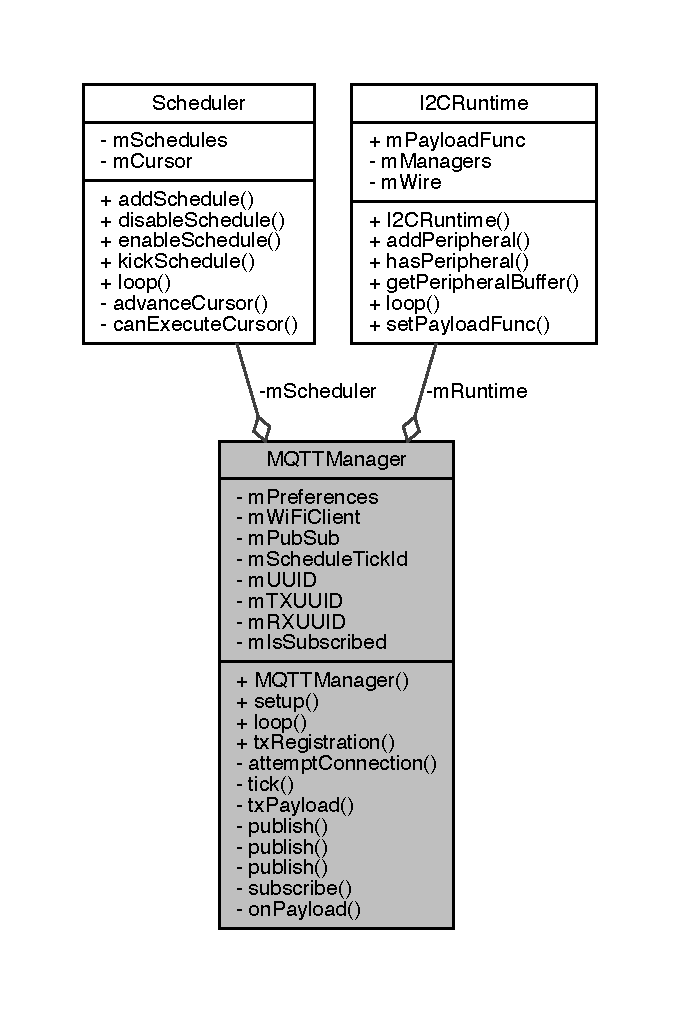
\includegraphics[width=326pt]{class_m_q_t_t_manager__coll__graph}
\end{center}
\end{figure}
\subsection*{Public Member Functions}
\begin{DoxyCompactItemize}
\item 
\mbox{\hyperlink{class_m_q_t_t_manager_af4a0454e2b8c10d989df9647c31611ad}{M\+Q\+T\+T\+Manager}} (\mbox{\hyperlink{class_i2_c_runtime}{I2\+C\+Runtime}} \&\mbox{\hyperlink{main_8cpp_a1fa047c23d7c85d1ad97022cd6b157d0}{runtime}})
\item 
void \mbox{\hyperlink{class_m_q_t_t_manager_a522f958b12d67c372a02c55ec0c24261}{setup}} ()
\item 
void \mbox{\hyperlink{class_m_q_t_t_manager_a9266e647933501851b411b6d2a9a1f95}{loop}} ()
\item 
void \mbox{\hyperlink{class_m_q_t_t_manager_aa7c667290f7d20e611f58de25b9b0354}{tx\+Registration}} (std\+::vector$<$ \mbox{\hyperlink{struct_peripheral_status}{Peripheral\+Status}} $>$ $\ast$statuses)
\end{DoxyCompactItemize}
\subsection*{Private Member Functions}
\begin{DoxyCompactItemize}
\item 
void \mbox{\hyperlink{class_m_q_t_t_manager_a99b5f971ca290bec4afe7d6da0003812}{attempt\+Connection}} ()
\item 
void \mbox{\hyperlink{class_m_q_t_t_manager_a19b077a9e80135537efee44963883b3c}{tick}} ()
\item 
void \mbox{\hyperlink{class_m_q_t_t_manager_a517bb71c7de061b711a025013564e232}{tx\+Payload}} (uint32\+\_\+t bus\+Id, uint16\+\_\+t bus\+Address, \mbox{\hyperlink{struct_read_definition}{Read\+Definition}} $\ast$def, uint8\+\_\+t $\ast$payload)
\item 
bool \mbox{\hyperlink{class_m_q_t_t_manager_a1559f6ac139c883032ecf9283304b3f4}{publish}} (uint8\+\_\+t $\ast$payload, unsigned int len)
\item 
bool \mbox{\hyperlink{class_m_q_t_t_manager_aba95650540cd217055d1e0b993988561}{publish}} (char $\ast$payload)
\item 
bool \mbox{\hyperlink{class_m_q_t_t_manager_aec3beb05d7f795b3334d9f9a5c9d9421}{publish}} (std\+::string payload)
\item 
void \mbox{\hyperlink{class_m_q_t_t_manager_ad714e14eda21ba3edb0957ccb6bf8ef4}{subscribe}} ()
\item 
void \mbox{\hyperlink{class_m_q_t_t_manager_a8e90a9d70e31ba4af28da5370d68902d}{on\+Payload}} (char $\ast$topic, uint8\+\_\+t $\ast$payload, unsigned int size)
\end{DoxyCompactItemize}
\subsection*{Private Attributes}
\begin{DoxyCompactItemize}
\item 
\mbox{\hyperlink{class_i2_c_runtime}{I2\+C\+Runtime}} \& \mbox{\hyperlink{class_m_q_t_t_manager_a3356cf93c237e44a28fbdc9e08e0b200}{m\+Runtime}}
\item 
Preferences \mbox{\hyperlink{class_m_q_t_t_manager_ab66bec340759e027dfa3ba3d37c1e6f7}{m\+Preferences}}
\item 
Wi\+Fi\+Client \mbox{\hyperlink{class_m_q_t_t_manager_af2d0eee7437193b3488b83e7afa56cd8}{m\+Wi\+Fi\+Client}}
\item 
Pub\+Sub\+Client \mbox{\hyperlink{class_m_q_t_t_manager_a7c702f0eda3bfa291a11591cebdaeed5}{m\+Pub\+Sub}}
\item 
\mbox{\hyperlink{class_scheduler}{Scheduler}} \mbox{\hyperlink{class_m_q_t_t_manager_aa6c36179bc117250fac8068de441775c}{m\+Scheduler}}
\item 
\mbox{\hyperlink{_scheduler_8h_a1e3b4605bdcbb8f6df7c47013e26e910}{Schedule\+Id}} \mbox{\hyperlink{class_m_q_t_t_manager_abce927e68d9a29836f6e24425a99e6fc}{m\+Schedule\+Tick\+Id}}
\item 
char \mbox{\hyperlink{class_m_q_t_t_manager_a5a9517149033c08d3915df0625da08ff}{m\+U\+U\+ID}} \mbox{[}13\mbox{]}
\item 
char \mbox{\hyperlink{class_m_q_t_t_manager_ad7c10e50256600dc9952501ac7a3eebb}{m\+T\+X\+U\+U\+ID}} \mbox{[}16\mbox{]}
\item 
char \mbox{\hyperlink{class_m_q_t_t_manager_ab03da55b905537f50873245b60944b8c}{m\+R\+X\+U\+U\+ID}} \mbox{[}16\mbox{]}
\item 
bool \mbox{\hyperlink{class_m_q_t_t_manager_a8c1e9df7f05ec6ca83421f4e2ad9fa33}{m\+Is\+Subscribed}}
\end{DoxyCompactItemize}


\subsection{Detailed Description}
Responsible for publishing and subscribing to topics on the M\+Q\+TT broker. 

\subsection{Constructor \& Destructor Documentation}
\mbox{\Hypertarget{class_m_q_t_t_manager_af4a0454e2b8c10d989df9647c31611ad}\label{class_m_q_t_t_manager_af4a0454e2b8c10d989df9647c31611ad}} 
\index{M\+Q\+T\+T\+Manager@{M\+Q\+T\+T\+Manager}!M\+Q\+T\+T\+Manager@{M\+Q\+T\+T\+Manager}}
\index{M\+Q\+T\+T\+Manager@{M\+Q\+T\+T\+Manager}!M\+Q\+T\+T\+Manager@{M\+Q\+T\+T\+Manager}}
\subsubsection{\texorpdfstring{M\+Q\+T\+T\+Manager()}{MQTTManager()}}
{\footnotesize\ttfamily M\+Q\+T\+T\+Manager\+::\+M\+Q\+T\+T\+Manager (\begin{DoxyParamCaption}\item[{\mbox{\hyperlink{class_i2_c_runtime}{I2\+C\+Runtime}} \&}]{runtime }\end{DoxyParamCaption})}



\subsection{Member Function Documentation}
\mbox{\Hypertarget{class_m_q_t_t_manager_a99b5f971ca290bec4afe7d6da0003812}\label{class_m_q_t_t_manager_a99b5f971ca290bec4afe7d6da0003812}} 
\index{M\+Q\+T\+T\+Manager@{M\+Q\+T\+T\+Manager}!attempt\+Connection@{attempt\+Connection}}
\index{attempt\+Connection@{attempt\+Connection}!M\+Q\+T\+T\+Manager@{M\+Q\+T\+T\+Manager}}
\subsubsection{\texorpdfstring{attempt\+Connection()}{attemptConnection()}}
{\footnotesize\ttfamily void M\+Q\+T\+T\+Manager\+::attempt\+Connection (\begin{DoxyParamCaption}{ }\end{DoxyParamCaption})\hspace{0.3cm}{\ttfamily [private]}}

\mbox{\Hypertarget{class_m_q_t_t_manager_a9266e647933501851b411b6d2a9a1f95}\label{class_m_q_t_t_manager_a9266e647933501851b411b6d2a9a1f95}} 
\index{M\+Q\+T\+T\+Manager@{M\+Q\+T\+T\+Manager}!loop@{loop}}
\index{loop@{loop}!M\+Q\+T\+T\+Manager@{M\+Q\+T\+T\+Manager}}
\subsubsection{\texorpdfstring{loop()}{loop()}}
{\footnotesize\ttfamily void M\+Q\+T\+T\+Manager\+::loop (\begin{DoxyParamCaption}{ }\end{DoxyParamCaption})}

\mbox{\Hypertarget{class_m_q_t_t_manager_a8e90a9d70e31ba4af28da5370d68902d}\label{class_m_q_t_t_manager_a8e90a9d70e31ba4af28da5370d68902d}} 
\index{M\+Q\+T\+T\+Manager@{M\+Q\+T\+T\+Manager}!on\+Payload@{on\+Payload}}
\index{on\+Payload@{on\+Payload}!M\+Q\+T\+T\+Manager@{M\+Q\+T\+T\+Manager}}
\subsubsection{\texorpdfstring{on\+Payload()}{onPayload()}}
{\footnotesize\ttfamily void M\+Q\+T\+T\+Manager\+::on\+Payload (\begin{DoxyParamCaption}\item[{char $\ast$}]{topic,  }\item[{uint8\+\_\+t $\ast$}]{payload,  }\item[{unsigned int}]{size }\end{DoxyParamCaption})\hspace{0.3cm}{\ttfamily [private]}}

\mbox{\Hypertarget{class_m_q_t_t_manager_a1559f6ac139c883032ecf9283304b3f4}\label{class_m_q_t_t_manager_a1559f6ac139c883032ecf9283304b3f4}} 
\index{M\+Q\+T\+T\+Manager@{M\+Q\+T\+T\+Manager}!publish@{publish}}
\index{publish@{publish}!M\+Q\+T\+T\+Manager@{M\+Q\+T\+T\+Manager}}
\subsubsection{\texorpdfstring{publish()}{publish()}\hspace{0.1cm}{\footnotesize\ttfamily [1/3]}}
{\footnotesize\ttfamily bool M\+Q\+T\+T\+Manager\+::publish (\begin{DoxyParamCaption}\item[{uint8\+\_\+t $\ast$}]{payload,  }\item[{unsigned int}]{len }\end{DoxyParamCaption})\hspace{0.3cm}{\ttfamily [private]}}

\mbox{\Hypertarget{class_m_q_t_t_manager_aba95650540cd217055d1e0b993988561}\label{class_m_q_t_t_manager_aba95650540cd217055d1e0b993988561}} 
\index{M\+Q\+T\+T\+Manager@{M\+Q\+T\+T\+Manager}!publish@{publish}}
\index{publish@{publish}!M\+Q\+T\+T\+Manager@{M\+Q\+T\+T\+Manager}}
\subsubsection{\texorpdfstring{publish()}{publish()}\hspace{0.1cm}{\footnotesize\ttfamily [2/3]}}
{\footnotesize\ttfamily bool M\+Q\+T\+T\+Manager\+::publish (\begin{DoxyParamCaption}\item[{char $\ast$}]{payload }\end{DoxyParamCaption})\hspace{0.3cm}{\ttfamily [private]}}

\mbox{\Hypertarget{class_m_q_t_t_manager_aec3beb05d7f795b3334d9f9a5c9d9421}\label{class_m_q_t_t_manager_aec3beb05d7f795b3334d9f9a5c9d9421}} 
\index{M\+Q\+T\+T\+Manager@{M\+Q\+T\+T\+Manager}!publish@{publish}}
\index{publish@{publish}!M\+Q\+T\+T\+Manager@{M\+Q\+T\+T\+Manager}}
\subsubsection{\texorpdfstring{publish()}{publish()}\hspace{0.1cm}{\footnotesize\ttfamily [3/3]}}
{\footnotesize\ttfamily bool M\+Q\+T\+T\+Manager\+::publish (\begin{DoxyParamCaption}\item[{std\+::string}]{payload }\end{DoxyParamCaption})\hspace{0.3cm}{\ttfamily [private]}}

\mbox{\Hypertarget{class_m_q_t_t_manager_a522f958b12d67c372a02c55ec0c24261}\label{class_m_q_t_t_manager_a522f958b12d67c372a02c55ec0c24261}} 
\index{M\+Q\+T\+T\+Manager@{M\+Q\+T\+T\+Manager}!setup@{setup}}
\index{setup@{setup}!M\+Q\+T\+T\+Manager@{M\+Q\+T\+T\+Manager}}
\subsubsection{\texorpdfstring{setup()}{setup()}}
{\footnotesize\ttfamily void M\+Q\+T\+T\+Manager\+::setup (\begin{DoxyParamCaption}{ }\end{DoxyParamCaption})}

\mbox{\Hypertarget{class_m_q_t_t_manager_ad714e14eda21ba3edb0957ccb6bf8ef4}\label{class_m_q_t_t_manager_ad714e14eda21ba3edb0957ccb6bf8ef4}} 
\index{M\+Q\+T\+T\+Manager@{M\+Q\+T\+T\+Manager}!subscribe@{subscribe}}
\index{subscribe@{subscribe}!M\+Q\+T\+T\+Manager@{M\+Q\+T\+T\+Manager}}
\subsubsection{\texorpdfstring{subscribe()}{subscribe()}}
{\footnotesize\ttfamily void M\+Q\+T\+T\+Manager\+::subscribe (\begin{DoxyParamCaption}{ }\end{DoxyParamCaption})\hspace{0.3cm}{\ttfamily [private]}}

\mbox{\Hypertarget{class_m_q_t_t_manager_a19b077a9e80135537efee44963883b3c}\label{class_m_q_t_t_manager_a19b077a9e80135537efee44963883b3c}} 
\index{M\+Q\+T\+T\+Manager@{M\+Q\+T\+T\+Manager}!tick@{tick}}
\index{tick@{tick}!M\+Q\+T\+T\+Manager@{M\+Q\+T\+T\+Manager}}
\subsubsection{\texorpdfstring{tick()}{tick()}}
{\footnotesize\ttfamily void M\+Q\+T\+T\+Manager\+::tick (\begin{DoxyParamCaption}{ }\end{DoxyParamCaption})\hspace{0.3cm}{\ttfamily [private]}}

\mbox{\Hypertarget{class_m_q_t_t_manager_a517bb71c7de061b711a025013564e232}\label{class_m_q_t_t_manager_a517bb71c7de061b711a025013564e232}} 
\index{M\+Q\+T\+T\+Manager@{M\+Q\+T\+T\+Manager}!tx\+Payload@{tx\+Payload}}
\index{tx\+Payload@{tx\+Payload}!M\+Q\+T\+T\+Manager@{M\+Q\+T\+T\+Manager}}
\subsubsection{\texorpdfstring{tx\+Payload()}{txPayload()}}
{\footnotesize\ttfamily void M\+Q\+T\+T\+Manager\+::tx\+Payload (\begin{DoxyParamCaption}\item[{uint32\+\_\+t}]{bus\+Id,  }\item[{uint16\+\_\+t}]{bus\+Address,  }\item[{\mbox{\hyperlink{struct_read_definition}{Read\+Definition}} $\ast$}]{def,  }\item[{uint8\+\_\+t $\ast$}]{payload }\end{DoxyParamCaption})\hspace{0.3cm}{\ttfamily [private]}}

\mbox{\Hypertarget{class_m_q_t_t_manager_aa7c667290f7d20e611f58de25b9b0354}\label{class_m_q_t_t_manager_aa7c667290f7d20e611f58de25b9b0354}} 
\index{M\+Q\+T\+T\+Manager@{M\+Q\+T\+T\+Manager}!tx\+Registration@{tx\+Registration}}
\index{tx\+Registration@{tx\+Registration}!M\+Q\+T\+T\+Manager@{M\+Q\+T\+T\+Manager}}
\subsubsection{\texorpdfstring{tx\+Registration()}{txRegistration()}}
{\footnotesize\ttfamily void M\+Q\+T\+T\+Manager\+::tx\+Registration (\begin{DoxyParamCaption}\item[{std\+::vector$<$ \mbox{\hyperlink{struct_peripheral_status}{Peripheral\+Status}} $>$ $\ast$}]{statuses }\end{DoxyParamCaption})}



\subsection{Member Data Documentation}
\mbox{\Hypertarget{class_m_q_t_t_manager_a8c1e9df7f05ec6ca83421f4e2ad9fa33}\label{class_m_q_t_t_manager_a8c1e9df7f05ec6ca83421f4e2ad9fa33}} 
\index{M\+Q\+T\+T\+Manager@{M\+Q\+T\+T\+Manager}!m\+Is\+Subscribed@{m\+Is\+Subscribed}}
\index{m\+Is\+Subscribed@{m\+Is\+Subscribed}!M\+Q\+T\+T\+Manager@{M\+Q\+T\+T\+Manager}}
\subsubsection{\texorpdfstring{m\+Is\+Subscribed}{mIsSubscribed}}
{\footnotesize\ttfamily bool M\+Q\+T\+T\+Manager\+::m\+Is\+Subscribed\hspace{0.3cm}{\ttfamily [private]}}

\mbox{\Hypertarget{class_m_q_t_t_manager_ab66bec340759e027dfa3ba3d37c1e6f7}\label{class_m_q_t_t_manager_ab66bec340759e027dfa3ba3d37c1e6f7}} 
\index{M\+Q\+T\+T\+Manager@{M\+Q\+T\+T\+Manager}!m\+Preferences@{m\+Preferences}}
\index{m\+Preferences@{m\+Preferences}!M\+Q\+T\+T\+Manager@{M\+Q\+T\+T\+Manager}}
\subsubsection{\texorpdfstring{m\+Preferences}{mPreferences}}
{\footnotesize\ttfamily Preferences M\+Q\+T\+T\+Manager\+::m\+Preferences\hspace{0.3cm}{\ttfamily [private]}}

\mbox{\Hypertarget{class_m_q_t_t_manager_a7c702f0eda3bfa291a11591cebdaeed5}\label{class_m_q_t_t_manager_a7c702f0eda3bfa291a11591cebdaeed5}} 
\index{M\+Q\+T\+T\+Manager@{M\+Q\+T\+T\+Manager}!m\+Pub\+Sub@{m\+Pub\+Sub}}
\index{m\+Pub\+Sub@{m\+Pub\+Sub}!M\+Q\+T\+T\+Manager@{M\+Q\+T\+T\+Manager}}
\subsubsection{\texorpdfstring{m\+Pub\+Sub}{mPubSub}}
{\footnotesize\ttfamily Pub\+Sub\+Client M\+Q\+T\+T\+Manager\+::m\+Pub\+Sub\hspace{0.3cm}{\ttfamily [private]}}

\mbox{\Hypertarget{class_m_q_t_t_manager_a3356cf93c237e44a28fbdc9e08e0b200}\label{class_m_q_t_t_manager_a3356cf93c237e44a28fbdc9e08e0b200}} 
\index{M\+Q\+T\+T\+Manager@{M\+Q\+T\+T\+Manager}!m\+Runtime@{m\+Runtime}}
\index{m\+Runtime@{m\+Runtime}!M\+Q\+T\+T\+Manager@{M\+Q\+T\+T\+Manager}}
\subsubsection{\texorpdfstring{m\+Runtime}{mRuntime}}
{\footnotesize\ttfamily \mbox{\hyperlink{class_i2_c_runtime}{I2\+C\+Runtime}}\& M\+Q\+T\+T\+Manager\+::m\+Runtime\hspace{0.3cm}{\ttfamily [private]}}

\mbox{\Hypertarget{class_m_q_t_t_manager_ab03da55b905537f50873245b60944b8c}\label{class_m_q_t_t_manager_ab03da55b905537f50873245b60944b8c}} 
\index{M\+Q\+T\+T\+Manager@{M\+Q\+T\+T\+Manager}!m\+R\+X\+U\+U\+ID@{m\+R\+X\+U\+U\+ID}}
\index{m\+R\+X\+U\+U\+ID@{m\+R\+X\+U\+U\+ID}!M\+Q\+T\+T\+Manager@{M\+Q\+T\+T\+Manager}}
\subsubsection{\texorpdfstring{m\+R\+X\+U\+U\+ID}{mRXUUID}}
{\footnotesize\ttfamily char M\+Q\+T\+T\+Manager\+::m\+R\+X\+U\+U\+ID\mbox{[}16\mbox{]}\hspace{0.3cm}{\ttfamily [private]}}

\mbox{\Hypertarget{class_m_q_t_t_manager_aa6c36179bc117250fac8068de441775c}\label{class_m_q_t_t_manager_aa6c36179bc117250fac8068de441775c}} 
\index{M\+Q\+T\+T\+Manager@{M\+Q\+T\+T\+Manager}!m\+Scheduler@{m\+Scheduler}}
\index{m\+Scheduler@{m\+Scheduler}!M\+Q\+T\+T\+Manager@{M\+Q\+T\+T\+Manager}}
\subsubsection{\texorpdfstring{m\+Scheduler}{mScheduler}}
{\footnotesize\ttfamily \mbox{\hyperlink{class_scheduler}{Scheduler}} M\+Q\+T\+T\+Manager\+::m\+Scheduler\hspace{0.3cm}{\ttfamily [private]}}

\mbox{\Hypertarget{class_m_q_t_t_manager_abce927e68d9a29836f6e24425a99e6fc}\label{class_m_q_t_t_manager_abce927e68d9a29836f6e24425a99e6fc}} 
\index{M\+Q\+T\+T\+Manager@{M\+Q\+T\+T\+Manager}!m\+Schedule\+Tick\+Id@{m\+Schedule\+Tick\+Id}}
\index{m\+Schedule\+Tick\+Id@{m\+Schedule\+Tick\+Id}!M\+Q\+T\+T\+Manager@{M\+Q\+T\+T\+Manager}}
\subsubsection{\texorpdfstring{m\+Schedule\+Tick\+Id}{mScheduleTickId}}
{\footnotesize\ttfamily \mbox{\hyperlink{_scheduler_8h_a1e3b4605bdcbb8f6df7c47013e26e910}{Schedule\+Id}} M\+Q\+T\+T\+Manager\+::m\+Schedule\+Tick\+Id\hspace{0.3cm}{\ttfamily [private]}}

\mbox{\Hypertarget{class_m_q_t_t_manager_ad7c10e50256600dc9952501ac7a3eebb}\label{class_m_q_t_t_manager_ad7c10e50256600dc9952501ac7a3eebb}} 
\index{M\+Q\+T\+T\+Manager@{M\+Q\+T\+T\+Manager}!m\+T\+X\+U\+U\+ID@{m\+T\+X\+U\+U\+ID}}
\index{m\+T\+X\+U\+U\+ID@{m\+T\+X\+U\+U\+ID}!M\+Q\+T\+T\+Manager@{M\+Q\+T\+T\+Manager}}
\subsubsection{\texorpdfstring{m\+T\+X\+U\+U\+ID}{mTXUUID}}
{\footnotesize\ttfamily char M\+Q\+T\+T\+Manager\+::m\+T\+X\+U\+U\+ID\mbox{[}16\mbox{]}\hspace{0.3cm}{\ttfamily [private]}}

\mbox{\Hypertarget{class_m_q_t_t_manager_a5a9517149033c08d3915df0625da08ff}\label{class_m_q_t_t_manager_a5a9517149033c08d3915df0625da08ff}} 
\index{M\+Q\+T\+T\+Manager@{M\+Q\+T\+T\+Manager}!m\+U\+U\+ID@{m\+U\+U\+ID}}
\index{m\+U\+U\+ID@{m\+U\+U\+ID}!M\+Q\+T\+T\+Manager@{M\+Q\+T\+T\+Manager}}
\subsubsection{\texorpdfstring{m\+U\+U\+ID}{mUUID}}
{\footnotesize\ttfamily char M\+Q\+T\+T\+Manager\+::m\+U\+U\+ID\mbox{[}13\mbox{]}\hspace{0.3cm}{\ttfamily [private]}}

\mbox{\Hypertarget{class_m_q_t_t_manager_af2d0eee7437193b3488b83e7afa56cd8}\label{class_m_q_t_t_manager_af2d0eee7437193b3488b83e7afa56cd8}} 
\index{M\+Q\+T\+T\+Manager@{M\+Q\+T\+T\+Manager}!m\+Wi\+Fi\+Client@{m\+Wi\+Fi\+Client}}
\index{m\+Wi\+Fi\+Client@{m\+Wi\+Fi\+Client}!M\+Q\+T\+T\+Manager@{M\+Q\+T\+T\+Manager}}
\subsubsection{\texorpdfstring{m\+Wi\+Fi\+Client}{mWiFiClient}}
{\footnotesize\ttfamily Wi\+Fi\+Client M\+Q\+T\+T\+Manager\+::m\+Wi\+Fi\+Client\hspace{0.3cm}{\ttfamily [private]}}



The documentation for this class was generated from the following files\+:\begin{DoxyCompactItemize}
\item 
include/\mbox{\hyperlink{_m_q_t_t_manager_8h}{M\+Q\+T\+T\+Manager.\+h}}\item 
src/\mbox{\hyperlink{_m_q_t_t_manager_8cpp}{M\+Q\+T\+T\+Manager.\+cpp}}\end{DoxyCompactItemize}

\hypertarget{struct_peripheral}{}\section{Peripheral Struct Reference}
\label{struct_peripheral}\index{Peripheral@{Peripheral}}


Declarative configuration for the behaviour of a peripheral on the I2C bus.  




{\ttfamily \#include $<$I2\+C\+Peripheral.\+h$>$}



Collaboration diagram for Peripheral\+:\nopagebreak
\begin{figure}[H]
\begin{center}
\leavevmode
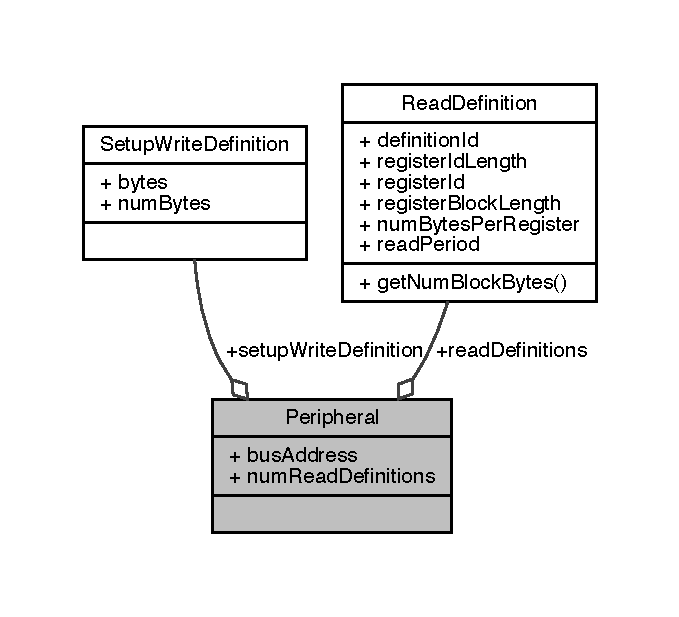
\includegraphics[width=326pt]{struct_peripheral__coll__graph}
\end{center}
\end{figure}
\subsection*{Public Attributes}
\begin{DoxyCompactItemize}
\item 
uint16\+\_\+t \mbox{\hyperlink{struct_peripheral_aeb9b037f7be4b84e967382c046077046}{bus\+Address}}
\item 
\mbox{\hyperlink{struct_setup_write_definition}{Setup\+Write\+Definition}} $\ast$ \mbox{\hyperlink{struct_peripheral_ab2a550bc5d7e03dcba843bf6f6367e12}{setup\+Write\+Definition}}
\item 
uint8\+\_\+t \mbox{\hyperlink{struct_peripheral_ae8a8523c12a7df87f2a0ebbce23658fe}{num\+Read\+Definitions}}
\item 
\mbox{\hyperlink{struct_read_definition}{Read\+Definition}} $\ast$$\ast$ \mbox{\hyperlink{struct_peripheral_a140bc115ee96fd0ab21ab1127beac7af}{read\+Definitions}}
\end{DoxyCompactItemize}


\subsection{Detailed Description}
Declarative configuration for the behaviour of a peripheral on the I2C bus. 

\subsection{Member Data Documentation}
\mbox{\Hypertarget{struct_peripheral_aeb9b037f7be4b84e967382c046077046}\label{struct_peripheral_aeb9b037f7be4b84e967382c046077046}} 
\index{Peripheral@{Peripheral}!bus\+Address@{bus\+Address}}
\index{bus\+Address@{bus\+Address}!Peripheral@{Peripheral}}
\subsubsection{\texorpdfstring{bus\+Address}{busAddress}}
{\footnotesize\ttfamily uint16\+\_\+t Peripheral\+::bus\+Address}

The address on the I2C bus. There is only one bus address per peripheral. This is not tied to {\ttfamily \mbox{\hyperlink{struct_read_definition}{Read\+Definition}}}s. \mbox{\Hypertarget{struct_peripheral_ae8a8523c12a7df87f2a0ebbce23658fe}\label{struct_peripheral_ae8a8523c12a7df87f2a0ebbce23658fe}} 
\index{Peripheral@{Peripheral}!num\+Read\+Definitions@{num\+Read\+Definitions}}
\index{num\+Read\+Definitions@{num\+Read\+Definitions}!Peripheral@{Peripheral}}
\subsubsection{\texorpdfstring{num\+Read\+Definitions}{numReadDefinitions}}
{\footnotesize\ttfamily uint8\+\_\+t Peripheral\+::num\+Read\+Definitions}

A \mbox{\hyperlink{struct_peripheral}{Peripheral}} can define multiple things to read. e.\+g., a peripheral may provide accelerometer and gyroscope data at non-\/contiguous register I\+Ds. \mbox{\Hypertarget{struct_peripheral_a140bc115ee96fd0ab21ab1127beac7af}\label{struct_peripheral_a140bc115ee96fd0ab21ab1127beac7af}} 
\index{Peripheral@{Peripheral}!read\+Definitions@{read\+Definitions}}
\index{read\+Definitions@{read\+Definitions}!Peripheral@{Peripheral}}
\subsubsection{\texorpdfstring{read\+Definitions}{readDefinitions}}
{\footnotesize\ttfamily \mbox{\hyperlink{struct_read_definition}{Read\+Definition}}$\ast$$\ast$ Peripheral\+::read\+Definitions}

\mbox{\Hypertarget{struct_peripheral_ab2a550bc5d7e03dcba843bf6f6367e12}\label{struct_peripheral_ab2a550bc5d7e03dcba843bf6f6367e12}} 
\index{Peripheral@{Peripheral}!setup\+Write\+Definition@{setup\+Write\+Definition}}
\index{setup\+Write\+Definition@{setup\+Write\+Definition}!Peripheral@{Peripheral}}
\subsubsection{\texorpdfstring{setup\+Write\+Definition}{setupWriteDefinition}}
{\footnotesize\ttfamily \mbox{\hyperlink{struct_setup_write_definition}{Setup\+Write\+Definition}}$\ast$ Peripheral\+::setup\+Write\+Definition}

Some peripherals require configuration in the form of bytes sent to the peripheral at startup. 

The documentation for this struct was generated from the following file\+:\begin{DoxyCompactItemize}
\item 
include/\mbox{\hyperlink{_i2_c_peripheral_8h}{I2\+C\+Peripheral.\+h}}\end{DoxyCompactItemize}

\hypertarget{struct_peripheral_status}{}\section{Peripheral\+Status Struct Reference}
\label{struct_peripheral_status}\index{Peripheral\+Status@{Peripheral\+Status}}


Intermediate object for protobuf encoding.  




{\ttfamily \#include $<$Telemetry\+Protocol.\+h$>$}



Collaboration diagram for Peripheral\+Status\+:\nopagebreak
\begin{figure}[H]
\begin{center}
\leavevmode
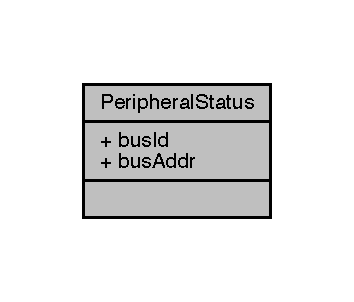
\includegraphics[width=170pt]{struct_peripheral_status__coll__graph}
\end{center}
\end{figure}
\subsection*{Public Attributes}
\begin{DoxyCompactItemize}
\item 
uint32\+\_\+t \mbox{\hyperlink{struct_peripheral_status_ad1d03bec7b4820fa7089ea59a61aa228}{bus\+Id}}
\item 
uint32\+\_\+t \mbox{\hyperlink{struct_peripheral_status_a02166b3f172d25857ce1e00a2c05ba7b}{bus\+Addr}}
\end{DoxyCompactItemize}


\subsection{Detailed Description}
Intermediate object for protobuf encoding. 

\subsection{Member Data Documentation}
\mbox{\Hypertarget{struct_peripheral_status_a02166b3f172d25857ce1e00a2c05ba7b}\label{struct_peripheral_status_a02166b3f172d25857ce1e00a2c05ba7b}} 
\index{Peripheral\+Status@{Peripheral\+Status}!bus\+Addr@{bus\+Addr}}
\index{bus\+Addr@{bus\+Addr}!Peripheral\+Status@{Peripheral\+Status}}
\subsubsection{\texorpdfstring{bus\+Addr}{busAddr}}
{\footnotesize\ttfamily uint32\+\_\+t Peripheral\+Status\+::bus\+Addr}

\mbox{\Hypertarget{struct_peripheral_status_ad1d03bec7b4820fa7089ea59a61aa228}\label{struct_peripheral_status_ad1d03bec7b4820fa7089ea59a61aa228}} 
\index{Peripheral\+Status@{Peripheral\+Status}!bus\+Id@{bus\+Id}}
\index{bus\+Id@{bus\+Id}!Peripheral\+Status@{Peripheral\+Status}}
\subsubsection{\texorpdfstring{bus\+Id}{busId}}
{\footnotesize\ttfamily uint32\+\_\+t Peripheral\+Status\+::bus\+Id}



The documentation for this struct was generated from the following file\+:\begin{DoxyCompactItemize}
\item 
include/\mbox{\hyperlink{_telemetry_protocol_8h}{Telemetry\+Protocol.\+h}}\end{DoxyCompactItemize}

\hypertarget{struct_read_definition}{}\section{Read\+Definition Struct Reference}
\label{struct_read_definition}\index{Read\+Definition@{Read\+Definition}}


Declarative configuration for reading a contiguous register block from a peripheral on the I2C bus.  




{\ttfamily \#include $<$I2\+C\+Peripheral.\+h$>$}



Collaboration diagram for Read\+Definition\+:\nopagebreak
\begin{figure}[H]
\begin{center}
\leavevmode
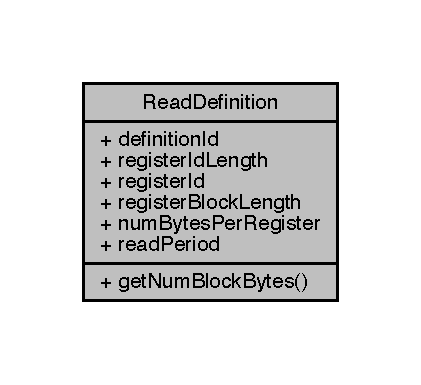
\includegraphics[width=202pt]{struct_read_definition__coll__graph}
\end{center}
\end{figure}
\subsection*{Public Member Functions}
\begin{DoxyCompactItemize}
\item 
uint16\+\_\+t \mbox{\hyperlink{struct_read_definition_a0cd8f09fd884f9d1f3c8638fafd47c82}{get\+Num\+Block\+Bytes}} ()
\end{DoxyCompactItemize}
\subsection*{Public Attributes}
\begin{DoxyCompactItemize}
\item 
uint16\+\_\+t \mbox{\hyperlink{struct_read_definition_ad38fa1092da3ab3fbc4543b306392b0e}{definition\+Id}}
\item 
\mbox{\hyperlink{_i2_c_peripheral_8h_ae0efcb4a72d88c76f03e57ed26b03383}{Register\+Length}} \mbox{\hyperlink{struct_read_definition_a842c09b580d962b7c8b8ce979c25c0e7}{register\+Id\+Length}}
\item 
uint16\+\_\+t \mbox{\hyperlink{struct_read_definition_af46d93354ce1dc2f413439b41b46eaa1}{register\+Id}}
\item 
uint8\+\_\+t \mbox{\hyperlink{struct_read_definition_a0b480fa0fee8d4651383ec6cf48bd7f0}{register\+Block\+Length}}
\item 
uint8\+\_\+t \mbox{\hyperlink{struct_read_definition_a3c13b2c7c3fb73632c856480621d32d6}{num\+Bytes\+Per\+Register}}
\item 
\mbox{\hyperlink{_scheduler_8h_aca1fa1a7edde6bf9e22c7617400fad31}{Duration}} \mbox{\hyperlink{struct_read_definition_aff14d6c02cce669e70bf4e7f45fb6ae0}{read\+Period}}
\end{DoxyCompactItemize}


\subsection{Detailed Description}
Declarative configuration for reading a contiguous register block from a peripheral on the I2C bus. 

\subsection{Member Function Documentation}
\mbox{\Hypertarget{struct_read_definition_a0cd8f09fd884f9d1f3c8638fafd47c82}\label{struct_read_definition_a0cd8f09fd884f9d1f3c8638fafd47c82}} 
\index{Read\+Definition@{Read\+Definition}!get\+Num\+Block\+Bytes@{get\+Num\+Block\+Bytes}}
\index{get\+Num\+Block\+Bytes@{get\+Num\+Block\+Bytes}!Read\+Definition@{Read\+Definition}}
\subsubsection{\texorpdfstring{get\+Num\+Block\+Bytes()}{getNumBlockBytes()}}
{\footnotesize\ttfamily uint16\+\_\+t Read\+Definition\+::get\+Num\+Block\+Bytes (\begin{DoxyParamCaption}{ }\end{DoxyParamCaption})}



\subsection{Member Data Documentation}
\mbox{\Hypertarget{struct_read_definition_ad38fa1092da3ab3fbc4543b306392b0e}\label{struct_read_definition_ad38fa1092da3ab3fbc4543b306392b0e}} 
\index{Read\+Definition@{Read\+Definition}!definition\+Id@{definition\+Id}}
\index{definition\+Id@{definition\+Id}!Read\+Definition@{Read\+Definition}}
\subsubsection{\texorpdfstring{definition\+Id}{definitionId}}
{\footnotesize\ttfamily uint16\+\_\+t Read\+Definition\+::definition\+Id}

An arbitrary ID for external reference. This does not relate to the hardware or any application logic in the \mbox{\hyperlink{class_i2_c_runtime}{I2\+C\+Runtime}}. This is used externally to track read definitions. \mbox{\Hypertarget{struct_read_definition_a3c13b2c7c3fb73632c856480621d32d6}\label{struct_read_definition_a3c13b2c7c3fb73632c856480621d32d6}} 
\index{Read\+Definition@{Read\+Definition}!num\+Bytes\+Per\+Register@{num\+Bytes\+Per\+Register}}
\index{num\+Bytes\+Per\+Register@{num\+Bytes\+Per\+Register}!Read\+Definition@{Read\+Definition}}
\subsubsection{\texorpdfstring{num\+Bytes\+Per\+Register}{numBytesPerRegister}}
{\footnotesize\ttfamily uint8\+\_\+t Read\+Definition\+::num\+Bytes\+Per\+Register}

The number of bytes that will be read at each register ID in the contiguous block. This means that the total number of bytes retrieved from one \mbox{\hyperlink{struct_read_definition}{Read\+Definition}} instance is\+: \begin{DoxyVerb}numBytesPerRegister * registerBlockLength\end{DoxyVerb}
 \mbox{\Hypertarget{struct_read_definition_aff14d6c02cce669e70bf4e7f45fb6ae0}\label{struct_read_definition_aff14d6c02cce669e70bf4e7f45fb6ae0}} 
\index{Read\+Definition@{Read\+Definition}!read\+Period@{read\+Period}}
\index{read\+Period@{read\+Period}!Read\+Definition@{Read\+Definition}}
\subsubsection{\texorpdfstring{read\+Period}{readPeriod}}
{\footnotesize\ttfamily \mbox{\hyperlink{_scheduler_8h_aca1fa1a7edde6bf9e22c7617400fad31}{Duration}} Read\+Definition\+::read\+Period}

How many milliseconds between reading all bytes from the block of registers? \mbox{\Hypertarget{struct_read_definition_a0b480fa0fee8d4651383ec6cf48bd7f0}\label{struct_read_definition_a0b480fa0fee8d4651383ec6cf48bd7f0}} 
\index{Read\+Definition@{Read\+Definition}!register\+Block\+Length@{register\+Block\+Length}}
\index{register\+Block\+Length@{register\+Block\+Length}!Read\+Definition@{Read\+Definition}}
\subsubsection{\texorpdfstring{register\+Block\+Length}{registerBlockLength}}
{\footnotesize\ttfamily uint8\+\_\+t Read\+Definition\+::register\+Block\+Length}

Data is read on this output from a contiguous block of register I\+Ds. e.\+g., 0x80 to 0x\+FF. This defines the number of register I\+Ds in the block. This is essentially how many times the loop will read bytes at a register and then advance to the next register. For many peripherals this value is simple 1 (i.\+e., there is no need to advance). \mbox{\Hypertarget{struct_read_definition_af46d93354ce1dc2f413439b41b46eaa1}\label{struct_read_definition_af46d93354ce1dc2f413439b41b46eaa1}} 
\index{Read\+Definition@{Read\+Definition}!register\+Id@{register\+Id}}
\index{register\+Id@{register\+Id}!Read\+Definition@{Read\+Definition}}
\subsubsection{\texorpdfstring{register\+Id}{registerId}}
{\footnotesize\ttfamily uint16\+\_\+t Read\+Definition\+::register\+Id}

Data is read on this output from a contiguous block of register I\+Ds. e.\+g., 0x80 to 0x\+FF. This is the first register ID of the block. \mbox{\Hypertarget{struct_read_definition_a842c09b580d962b7c8b8ce979c25c0e7}\label{struct_read_definition_a842c09b580d962b7c8b8ce979c25c0e7}} 
\index{Read\+Definition@{Read\+Definition}!register\+Id\+Length@{register\+Id\+Length}}
\index{register\+Id\+Length@{register\+Id\+Length}!Read\+Definition@{Read\+Definition}}
\subsubsection{\texorpdfstring{register\+Id\+Length}{registerIdLength}}
{\footnotesize\ttfamily \mbox{\hyperlink{_i2_c_peripheral_8h_ae0efcb4a72d88c76f03e57ed26b03383}{Register\+Length}} Read\+Definition\+::register\+Id\+Length}

Some peripherals have 16-\/bit register I\+Ds and some have 8-\/bit register I\+Ds. 

The documentation for this struct was generated from the following files\+:\begin{DoxyCompactItemize}
\item 
include/\mbox{\hyperlink{_i2_c_peripheral_8h}{I2\+C\+Peripheral.\+h}}\item 
src/\mbox{\hyperlink{_i2_c_runtime_8cpp}{I2\+C\+Runtime.\+cpp}}\end{DoxyCompactItemize}

\hypertarget{struct_schedule}{}\section{Schedule Struct Reference}
\label{struct_schedule}\index{Schedule@{Schedule}}


Declarative configuration for a managed schedule.  




{\ttfamily \#include $<$Scheduler.\+h$>$}



Collaboration diagram for Schedule\+:\nopagebreak
\begin{figure}[H]
\begin{center}
\leavevmode
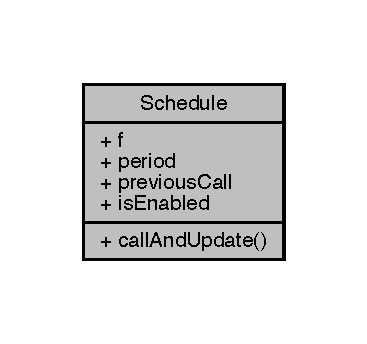
\includegraphics[width=176pt]{struct_schedule__coll__graph}
\end{center}
\end{figure}
\subsection*{Public Member Functions}
\begin{DoxyCompactItemize}
\item 
void \mbox{\hyperlink{struct_schedule_a13d8ce84c7b38bf5366e5512e2a55e23}{call\+And\+Update}} ()
\end{DoxyCompactItemize}
\subsection*{Public Attributes}
\begin{DoxyCompactItemize}
\item 
std\+::shared\+\_\+ptr$<$ \mbox{\hyperlink{_scheduler_8h_a2125a5a2949d6ee13163b671159c0d4d}{Func}} $>$ \mbox{\hyperlink{struct_schedule_a9d9c9f5ecb6213eea85e061b900ac398}{f}}
\item 
\mbox{\hyperlink{_scheduler_8h_aca1fa1a7edde6bf9e22c7617400fad31}{Duration}} \mbox{\hyperlink{struct_schedule_a63741d77dabb232150e334168a4c72c2}{period}}
\item 
\mbox{\hyperlink{_scheduler_8h_a67c6ac2398ae81344762ebb1b71fc9a7}{Timestamp}} \mbox{\hyperlink{struct_schedule_ab512e16f533bdc7a1c9d8c5c2bad0f7a}{previous\+Call}}
\item 
bool \mbox{\hyperlink{struct_schedule_a799716253aaa56ab67ceacee1a727a28}{is\+Enabled}}
\end{DoxyCompactItemize}


\subsection{Detailed Description}
Declarative configuration for a managed schedule. 

\subsection{Member Function Documentation}
\mbox{\Hypertarget{struct_schedule_a13d8ce84c7b38bf5366e5512e2a55e23}\label{struct_schedule_a13d8ce84c7b38bf5366e5512e2a55e23}} 
\index{Schedule@{Schedule}!call\+And\+Update@{call\+And\+Update}}
\index{call\+And\+Update@{call\+And\+Update}!Schedule@{Schedule}}
\subsubsection{\texorpdfstring{call\+And\+Update()}{callAndUpdate()}}
{\footnotesize\ttfamily void Schedule\+::call\+And\+Update (\begin{DoxyParamCaption}{ }\end{DoxyParamCaption})}



\subsection{Member Data Documentation}
\mbox{\Hypertarget{struct_schedule_a9d9c9f5ecb6213eea85e061b900ac398}\label{struct_schedule_a9d9c9f5ecb6213eea85e061b900ac398}} 
\index{Schedule@{Schedule}!f@{f}}
\index{f@{f}!Schedule@{Schedule}}
\subsubsection{\texorpdfstring{f}{f}}
{\footnotesize\ttfamily std\+::shared\+\_\+ptr$<$\mbox{\hyperlink{_scheduler_8h_a2125a5a2949d6ee13163b671159c0d4d}{Func}}$>$ Schedule\+::f}

\mbox{\Hypertarget{struct_schedule_a799716253aaa56ab67ceacee1a727a28}\label{struct_schedule_a799716253aaa56ab67ceacee1a727a28}} 
\index{Schedule@{Schedule}!is\+Enabled@{is\+Enabled}}
\index{is\+Enabled@{is\+Enabled}!Schedule@{Schedule}}
\subsubsection{\texorpdfstring{is\+Enabled}{isEnabled}}
{\footnotesize\ttfamily bool Schedule\+::is\+Enabled}

\mbox{\Hypertarget{struct_schedule_a63741d77dabb232150e334168a4c72c2}\label{struct_schedule_a63741d77dabb232150e334168a4c72c2}} 
\index{Schedule@{Schedule}!period@{period}}
\index{period@{period}!Schedule@{Schedule}}
\subsubsection{\texorpdfstring{period}{period}}
{\footnotesize\ttfamily \mbox{\hyperlink{_scheduler_8h_aca1fa1a7edde6bf9e22c7617400fad31}{Duration}} Schedule\+::period}

How many milliseconds between executions of {\ttfamily f}? \mbox{\Hypertarget{struct_schedule_ab512e16f533bdc7a1c9d8c5c2bad0f7a}\label{struct_schedule_ab512e16f533bdc7a1c9d8c5c2bad0f7a}} 
\index{Schedule@{Schedule}!previous\+Call@{previous\+Call}}
\index{previous\+Call@{previous\+Call}!Schedule@{Schedule}}
\subsubsection{\texorpdfstring{previous\+Call}{previousCall}}
{\footnotesize\ttfamily \mbox{\hyperlink{_scheduler_8h_a67c6ac2398ae81344762ebb1b71fc9a7}{Timestamp}} Schedule\+::previous\+Call}

When was the previous call of {\ttfamily f}? If {\ttfamily f} has never been called then this will be {\ttfamily H\+A\+S\+\_\+\+N\+E\+V\+E\+R\+\_\+\+R\+A\+N\+\_\+\+T\+I\+M\+E\+S\+T\+A\+MP}. 

The documentation for this struct was generated from the following files\+:\begin{DoxyCompactItemize}
\item 
include/\mbox{\hyperlink{_scheduler_8h}{Scheduler.\+h}}\item 
src/\mbox{\hyperlink{_scheduler_8cpp}{Scheduler.\+cpp}}\end{DoxyCompactItemize}

\hypertarget{class_scheduler}{}\section{Scheduler Class Reference}
\label{class_scheduler}\index{Scheduler@{Scheduler}}


Generic scheduler for non-\/blocking tasks given schedules for callbacks.  




{\ttfamily \#include $<$Scheduler.\+h$>$}



Collaboration diagram for Scheduler\+:\nopagebreak
\begin{figure}[H]
\begin{center}
\leavevmode
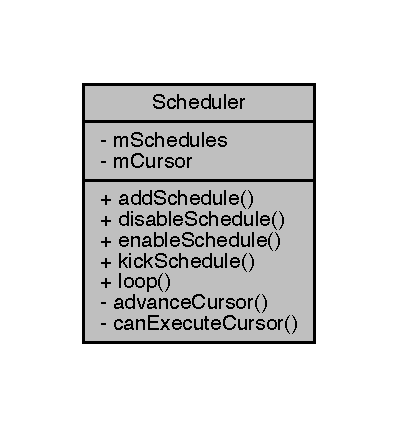
\includegraphics[width=191pt]{class_scheduler__coll__graph}
\end{center}
\end{figure}
\subsection*{Public Member Functions}
\begin{DoxyCompactItemize}
\item 
\mbox{\hyperlink{_scheduler_8h_a1e3b4605bdcbb8f6df7c47013e26e910}{Schedule\+Id}} \mbox{\hyperlink{class_scheduler_a28d9d19644657da9902e52f2901fbc15}{add\+Schedule}} (std\+::shared\+\_\+ptr$<$ \mbox{\hyperlink{_scheduler_8h_a2125a5a2949d6ee13163b671159c0d4d}{Func}} $>$, \mbox{\hyperlink{_scheduler_8h_aca1fa1a7edde6bf9e22c7617400fad31}{Duration}}, bool is\+Enabled=true)
\item 
void \mbox{\hyperlink{class_scheduler_a552dae97cbcd7c621f793311cf151717}{disable\+Schedule}} (\mbox{\hyperlink{_scheduler_8h_a1e3b4605bdcbb8f6df7c47013e26e910}{Schedule\+Id}})
\item 
void \mbox{\hyperlink{class_scheduler_a9df1991d93b673de51cbb4a9d15fe985}{enable\+Schedule}} (\mbox{\hyperlink{_scheduler_8h_a1e3b4605bdcbb8f6df7c47013e26e910}{Schedule\+Id}})
\item 
void \mbox{\hyperlink{class_scheduler_a7d3c44c9a4ca6c35e9970f3c67ac1349}{kick\+Schedule}} (\mbox{\hyperlink{_scheduler_8h_a1e3b4605bdcbb8f6df7c47013e26e910}{Schedule\+Id}})
\item 
void \mbox{\hyperlink{class_scheduler_a81607abe2905dee2e7cf9222a9e35b8f}{loop}} ()
\end{DoxyCompactItemize}
\subsection*{Private Member Functions}
\begin{DoxyCompactItemize}
\item 
void \mbox{\hyperlink{class_scheduler_ac44493a482b70bbe93a296a910377a2d}{advance\+Cursor}} ()
\item 
bool \mbox{\hyperlink{class_scheduler_a83c09d5b44ccce582ac2b699b1808a0f}{can\+Execute\+Cursor}} ()
\end{DoxyCompactItemize}
\subsection*{Private Attributes}
\begin{DoxyCompactItemize}
\item 
std\+::vector$<$ \mbox{\hyperlink{struct_schedule}{Schedule}} $>$ \mbox{\hyperlink{class_scheduler_a785bcdb6ecc1f238540e554e45aace7c}{m\+Schedules}}
\item 
std\+::vector$<$ \mbox{\hyperlink{struct_schedule}{Schedule}} $>$\+::iterator \mbox{\hyperlink{class_scheduler_a34d96eedc75db87662e70cc2c3ee0263}{m\+Cursor}}
\end{DoxyCompactItemize}


\subsection{Detailed Description}
Generic scheduler for non-\/blocking tasks given schedules for callbacks. 

\subsection{Member Function Documentation}
\mbox{\Hypertarget{class_scheduler_a28d9d19644657da9902e52f2901fbc15}\label{class_scheduler_a28d9d19644657da9902e52f2901fbc15}} 
\index{Scheduler@{Scheduler}!add\+Schedule@{add\+Schedule}}
\index{add\+Schedule@{add\+Schedule}!Scheduler@{Scheduler}}
\subsubsection{\texorpdfstring{add\+Schedule()}{addSchedule()}}
{\footnotesize\ttfamily \mbox{\hyperlink{_scheduler_8h_a1e3b4605bdcbb8f6df7c47013e26e910}{Schedule\+Id}} Scheduler\+::add\+Schedule (\begin{DoxyParamCaption}\item[{std\+::shared\+\_\+ptr$<$ \mbox{\hyperlink{_scheduler_8h_a2125a5a2949d6ee13163b671159c0d4d}{Func}} $>$}]{f,  }\item[{\mbox{\hyperlink{_scheduler_8h_aca1fa1a7edde6bf9e22c7617400fad31}{Duration}}}]{period,  }\item[{bool}]{is\+Enabled = {\ttfamily true} }\end{DoxyParamCaption})}

\mbox{\Hypertarget{class_scheduler_ac44493a482b70bbe93a296a910377a2d}\label{class_scheduler_ac44493a482b70bbe93a296a910377a2d}} 
\index{Scheduler@{Scheduler}!advance\+Cursor@{advance\+Cursor}}
\index{advance\+Cursor@{advance\+Cursor}!Scheduler@{Scheduler}}
\subsubsection{\texorpdfstring{advance\+Cursor()}{advanceCursor()}}
{\footnotesize\ttfamily void Scheduler\+::advance\+Cursor (\begin{DoxyParamCaption}{ }\end{DoxyParamCaption})\hspace{0.3cm}{\ttfamily [private]}}

\mbox{\Hypertarget{class_scheduler_a83c09d5b44ccce582ac2b699b1808a0f}\label{class_scheduler_a83c09d5b44ccce582ac2b699b1808a0f}} 
\index{Scheduler@{Scheduler}!can\+Execute\+Cursor@{can\+Execute\+Cursor}}
\index{can\+Execute\+Cursor@{can\+Execute\+Cursor}!Scheduler@{Scheduler}}
\subsubsection{\texorpdfstring{can\+Execute\+Cursor()}{canExecuteCursor()}}
{\footnotesize\ttfamily bool Scheduler\+::can\+Execute\+Cursor (\begin{DoxyParamCaption}{ }\end{DoxyParamCaption})\hspace{0.3cm}{\ttfamily [private]}}

\mbox{\Hypertarget{class_scheduler_a552dae97cbcd7c621f793311cf151717}\label{class_scheduler_a552dae97cbcd7c621f793311cf151717}} 
\index{Scheduler@{Scheduler}!disable\+Schedule@{disable\+Schedule}}
\index{disable\+Schedule@{disable\+Schedule}!Scheduler@{Scheduler}}
\subsubsection{\texorpdfstring{disable\+Schedule()}{disableSchedule()}}
{\footnotesize\ttfamily void Scheduler\+::disable\+Schedule (\begin{DoxyParamCaption}\item[{\mbox{\hyperlink{_scheduler_8h_a1e3b4605bdcbb8f6df7c47013e26e910}{Schedule\+Id}}}]{id }\end{DoxyParamCaption})}

\mbox{\Hypertarget{class_scheduler_a9df1991d93b673de51cbb4a9d15fe985}\label{class_scheduler_a9df1991d93b673de51cbb4a9d15fe985}} 
\index{Scheduler@{Scheduler}!enable\+Schedule@{enable\+Schedule}}
\index{enable\+Schedule@{enable\+Schedule}!Scheduler@{Scheduler}}
\subsubsection{\texorpdfstring{enable\+Schedule()}{enableSchedule()}}
{\footnotesize\ttfamily void Scheduler\+::enable\+Schedule (\begin{DoxyParamCaption}\item[{\mbox{\hyperlink{_scheduler_8h_a1e3b4605bdcbb8f6df7c47013e26e910}{Schedule\+Id}}}]{id }\end{DoxyParamCaption})}

\mbox{\Hypertarget{class_scheduler_a7d3c44c9a4ca6c35e9970f3c67ac1349}\label{class_scheduler_a7d3c44c9a4ca6c35e9970f3c67ac1349}} 
\index{Scheduler@{Scheduler}!kick\+Schedule@{kick\+Schedule}}
\index{kick\+Schedule@{kick\+Schedule}!Scheduler@{Scheduler}}
\subsubsection{\texorpdfstring{kick\+Schedule()}{kickSchedule()}}
{\footnotesize\ttfamily void Scheduler\+::kick\+Schedule (\begin{DoxyParamCaption}\item[{\mbox{\hyperlink{_scheduler_8h_a1e3b4605bdcbb8f6df7c47013e26e910}{Schedule\+Id}}}]{id }\end{DoxyParamCaption})}

Update the schedule such that it will run after its period relative to the call of {\ttfamily kick\+Schedule}. e.\+g., if {\ttfamily kick\+Schedule} is called at t = 40 with a period of 500 then the schedule will be executed at t = 540. \mbox{\Hypertarget{class_scheduler_a81607abe2905dee2e7cf9222a9e35b8f}\label{class_scheduler_a81607abe2905dee2e7cf9222a9e35b8f}} 
\index{Scheduler@{Scheduler}!loop@{loop}}
\index{loop@{loop}!Scheduler@{Scheduler}}
\subsubsection{\texorpdfstring{loop()}{loop()}}
{\footnotesize\ttfamily void Scheduler\+::loop (\begin{DoxyParamCaption}{ }\end{DoxyParamCaption})}

This call should be non-\/blocking and consume as little C\+PU time as possible per execution. {\ttfamily m\+Cursor} is used to cycle through the schedules and check one schedule for execution per call. 

\subsection{Member Data Documentation}
\mbox{\Hypertarget{class_scheduler_a34d96eedc75db87662e70cc2c3ee0263}\label{class_scheduler_a34d96eedc75db87662e70cc2c3ee0263}} 
\index{Scheduler@{Scheduler}!m\+Cursor@{m\+Cursor}}
\index{m\+Cursor@{m\+Cursor}!Scheduler@{Scheduler}}
\subsubsection{\texorpdfstring{m\+Cursor}{mCursor}}
{\footnotesize\ttfamily std\+::vector$<$\mbox{\hyperlink{struct_schedule}{Schedule}}$>$\+::iterator Scheduler\+::m\+Cursor\hspace{0.3cm}{\ttfamily [private]}}

\mbox{\Hypertarget{class_scheduler_a785bcdb6ecc1f238540e554e45aace7c}\label{class_scheduler_a785bcdb6ecc1f238540e554e45aace7c}} 
\index{Scheduler@{Scheduler}!m\+Schedules@{m\+Schedules}}
\index{m\+Schedules@{m\+Schedules}!Scheduler@{Scheduler}}
\subsubsection{\texorpdfstring{m\+Schedules}{mSchedules}}
{\footnotesize\ttfamily std\+::vector$<$\mbox{\hyperlink{struct_schedule}{Schedule}}$>$ Scheduler\+::m\+Schedules\hspace{0.3cm}{\ttfamily [private]}}



The documentation for this class was generated from the following files\+:\begin{DoxyCompactItemize}
\item 
include/\mbox{\hyperlink{_scheduler_8h}{Scheduler.\+h}}\item 
src/\mbox{\hyperlink{_scheduler_8cpp}{Scheduler.\+cpp}}\end{DoxyCompactItemize}

\hypertarget{struct_setup_write_definition}{}\section{Setup\+Write\+Definition Struct Reference}
\label{struct_setup_write_definition}\index{Setup\+Write\+Definition@{Setup\+Write\+Definition}}


{\ttfamily \#include $<$I2\+C\+Peripheral.\+h$>$}



Collaboration diagram for Setup\+Write\+Definition\+:\nopagebreak
\begin{figure}[H]
\begin{center}
\leavevmode
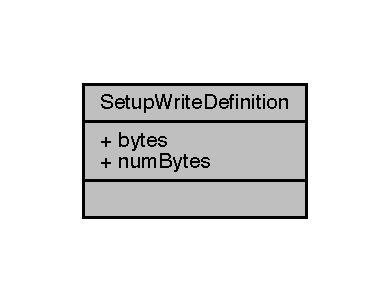
\includegraphics[width=187pt]{struct_setup_write_definition__coll__graph}
\end{center}
\end{figure}
\subsection*{Public Attributes}
\begin{DoxyCompactItemize}
\item 
uint8\+\_\+t $\ast$ \mbox{\hyperlink{struct_setup_write_definition_ac481b18396a89bfa8e9b4960316fb96e}{bytes}}
\item 
uint8\+\_\+t \mbox{\hyperlink{struct_setup_write_definition_ac106abf7ef3fbc971150c5ed427a8761}{num\+Bytes}}
\end{DoxyCompactItemize}


\subsection{Member Data Documentation}
\mbox{\Hypertarget{struct_setup_write_definition_ac481b18396a89bfa8e9b4960316fb96e}\label{struct_setup_write_definition_ac481b18396a89bfa8e9b4960316fb96e}} 
\index{Setup\+Write\+Definition@{Setup\+Write\+Definition}!bytes@{bytes}}
\index{bytes@{bytes}!Setup\+Write\+Definition@{Setup\+Write\+Definition}}
\subsubsection{\texorpdfstring{bytes}{bytes}}
{\footnotesize\ttfamily uint8\+\_\+t$\ast$ Setup\+Write\+Definition\+::bytes}

\mbox{\Hypertarget{struct_setup_write_definition_ac106abf7ef3fbc971150c5ed427a8761}\label{struct_setup_write_definition_ac106abf7ef3fbc971150c5ed427a8761}} 
\index{Setup\+Write\+Definition@{Setup\+Write\+Definition}!num\+Bytes@{num\+Bytes}}
\index{num\+Bytes@{num\+Bytes}!Setup\+Write\+Definition@{Setup\+Write\+Definition}}
\subsubsection{\texorpdfstring{num\+Bytes}{numBytes}}
{\footnotesize\ttfamily uint8\+\_\+t Setup\+Write\+Definition\+::num\+Bytes}



The documentation for this struct was generated from the following file\+:\begin{DoxyCompactItemize}
\item 
include/\mbox{\hyperlink{_i2_c_peripheral_8h}{I2\+C\+Peripheral.\+h}}\end{DoxyCompactItemize}

\hypertarget{struct_sized}{}\section{Sized Struct Reference}
\label{struct_sized}\index{Sized@{Sized}}


Buffer/size pair.  




Collaboration diagram for Sized\+:\nopagebreak
\begin{figure}[H]
\begin{center}
\leavevmode
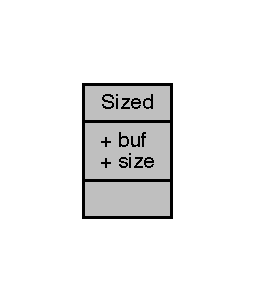
\includegraphics[width=122pt]{struct_sized__coll__graph}
\end{center}
\end{figure}
\subsection*{Public Attributes}
\begin{DoxyCompactItemize}
\item 
const uint8\+\_\+t $\ast$ \mbox{\hyperlink{struct_sized_a5513bffc6e24210df9a9bb93554bc556}{buf}}
\item 
size\+\_\+t \mbox{\hyperlink{struct_sized_a12b4432b66bb13986309dd678d3ad4b7}{size}}
\end{DoxyCompactItemize}


\subsection{Detailed Description}
Buffer/size pair. 

\subsection{Member Data Documentation}
\mbox{\Hypertarget{struct_sized_a5513bffc6e24210df9a9bb93554bc556}\label{struct_sized_a5513bffc6e24210df9a9bb93554bc556}} 
\index{Sized@{Sized}!buf@{buf}}
\index{buf@{buf}!Sized@{Sized}}
\subsubsection{\texorpdfstring{buf}{buf}}
{\footnotesize\ttfamily const uint8\+\_\+t$\ast$ Sized\+::buf}

\mbox{\Hypertarget{struct_sized_a12b4432b66bb13986309dd678d3ad4b7}\label{struct_sized_a12b4432b66bb13986309dd678d3ad4b7}} 
\index{Sized@{Sized}!size@{size}}
\index{size@{size}!Sized@{Sized}}
\subsubsection{\texorpdfstring{size}{size}}
{\footnotesize\ttfamily size\+\_\+t Sized\+::size}



The documentation for this struct was generated from the following file\+:\begin{DoxyCompactItemize}
\item 
src/\mbox{\hyperlink{_telemetry_protocol_8cc}{Telemetry\+Protocol.\+cc}}\end{DoxyCompactItemize}

\hypertarget{class_telemetry_protocol}{}\section{Telemetry\+Protocol Class Reference}
\label{class_telemetry_protocol}\index{Telemetry\+Protocol@{Telemetry\+Protocol}}


Responsible for encoding and decoding protobuf/nanopb payloads.  




{\ttfamily \#include $<$Telemetry\+Protocol.\+h$>$}



Collaboration diagram for Telemetry\+Protocol\+:\nopagebreak
\begin{figure}[H]
\begin{center}
\leavevmode
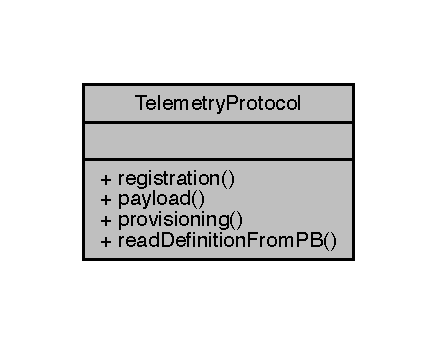
\includegraphics[width=210pt]{class_telemetry_protocol__coll__graph}
\end{center}
\end{figure}
\subsection*{Static Public Member Functions}
\begin{DoxyCompactItemize}
\item 
static size\+\_\+t \mbox{\hyperlink{class_telemetry_protocol_ad8584639767a19015907168116f21c4b}{registration}} (std\+::vector$<$ \mbox{\hyperlink{struct_peripheral_status}{Peripheral\+Status}} $>$ $\ast$statuses, uint8\+\_\+t $\ast$buffer)
\item 
static size\+\_\+t \mbox{\hyperlink{class_telemetry_protocol_a9b14fc6a3f0942bdc9d91e45604c082a}{payload}} (uint32\+\_\+t bus\+Id, uint16\+\_\+t bus\+Address, \mbox{\hyperlink{struct_read_definition}{Read\+Definition}} $\ast$def, uint8\+\_\+t $\ast$payload, uint8\+\_\+t $\ast$buffer)
\item 
static \mbox{\hyperlink{struct_peripheral}{Peripheral}} $\ast$ \mbox{\hyperlink{class_telemetry_protocol_a2425d455bed0b9b994c1de41b334fca5}{provisioning}} (uint8\+\_\+t $\ast$buffer, unsigned int size)
\item 
static \mbox{\hyperlink{struct_read_definition}{Read\+Definition}} $\ast$ \mbox{\hyperlink{class_telemetry_protocol_a90e74801cf6d35be65276720839165ab}{read\+Definition\+From\+PB}} (Provisioning\+\_\+\+Read\+Def \&msg)
\end{DoxyCompactItemize}


\subsection{Detailed Description}
Responsible for encoding and decoding protobuf/nanopb payloads. 

\subsection{Member Function Documentation}
\mbox{\Hypertarget{class_telemetry_protocol_a9b14fc6a3f0942bdc9d91e45604c082a}\label{class_telemetry_protocol_a9b14fc6a3f0942bdc9d91e45604c082a}} 
\index{Telemetry\+Protocol@{Telemetry\+Protocol}!payload@{payload}}
\index{payload@{payload}!Telemetry\+Protocol@{Telemetry\+Protocol}}
\subsubsection{\texorpdfstring{payload()}{payload()}}
{\footnotesize\ttfamily size\+\_\+t Telemetry\+Protocol\+::payload (\begin{DoxyParamCaption}\item[{uint32\+\_\+t}]{bus\+Id,  }\item[{uint16\+\_\+t}]{bus\+Address,  }\item[{\mbox{\hyperlink{struct_read_definition}{Read\+Definition}} $\ast$}]{def,  }\item[{uint8\+\_\+t $\ast$}]{payload,  }\item[{uint8\+\_\+t $\ast$}]{buffer }\end{DoxyParamCaption})\hspace{0.3cm}{\ttfamily [static]}}

\mbox{\Hypertarget{class_telemetry_protocol_a2425d455bed0b9b994c1de41b334fca5}\label{class_telemetry_protocol_a2425d455bed0b9b994c1de41b334fca5}} 
\index{Telemetry\+Protocol@{Telemetry\+Protocol}!provisioning@{provisioning}}
\index{provisioning@{provisioning}!Telemetry\+Protocol@{Telemetry\+Protocol}}
\subsubsection{\texorpdfstring{provisioning()}{provisioning()}}
{\footnotesize\ttfamily \mbox{\hyperlink{struct_peripheral}{Peripheral}} $\ast$ Telemetry\+Protocol\+::provisioning (\begin{DoxyParamCaption}\item[{uint8\+\_\+t $\ast$}]{buffer,  }\item[{unsigned int}]{size }\end{DoxyParamCaption})\hspace{0.3cm}{\ttfamily [static]}}

\mbox{\Hypertarget{class_telemetry_protocol_a90e74801cf6d35be65276720839165ab}\label{class_telemetry_protocol_a90e74801cf6d35be65276720839165ab}} 
\index{Telemetry\+Protocol@{Telemetry\+Protocol}!read\+Definition\+From\+PB@{read\+Definition\+From\+PB}}
\index{read\+Definition\+From\+PB@{read\+Definition\+From\+PB}!Telemetry\+Protocol@{Telemetry\+Protocol}}
\subsubsection{\texorpdfstring{read\+Definition\+From\+P\+B()}{readDefinitionFromPB()}}
{\footnotesize\ttfamily \mbox{\hyperlink{struct_read_definition}{Read\+Definition}} $\ast$ Telemetry\+Protocol\+::read\+Definition\+From\+PB (\begin{DoxyParamCaption}\item[{Provisioning\+\_\+\+Read\+Def \&}]{msg }\end{DoxyParamCaption})\hspace{0.3cm}{\ttfamily [static]}}

\mbox{\Hypertarget{class_telemetry_protocol_ad8584639767a19015907168116f21c4b}\label{class_telemetry_protocol_ad8584639767a19015907168116f21c4b}} 
\index{Telemetry\+Protocol@{Telemetry\+Protocol}!registration@{registration}}
\index{registration@{registration}!Telemetry\+Protocol@{Telemetry\+Protocol}}
\subsubsection{\texorpdfstring{registration()}{registration()}}
{\footnotesize\ttfamily size\+\_\+t Telemetry\+Protocol\+::registration (\begin{DoxyParamCaption}\item[{std\+::vector$<$ \mbox{\hyperlink{struct_peripheral_status}{Peripheral\+Status}} $>$ $\ast$}]{statuses,  }\item[{uint8\+\_\+t $\ast$}]{buffer }\end{DoxyParamCaption})\hspace{0.3cm}{\ttfamily [static]}}



The documentation for this class was generated from the following files\+:\begin{DoxyCompactItemize}
\item 
include/\mbox{\hyperlink{_telemetry_protocol_8h}{Telemetry\+Protocol.\+h}}\item 
src/\mbox{\hyperlink{_telemetry_protocol_8cc}{Telemetry\+Protocol.\+cc}}\end{DoxyCompactItemize}

\hypertarget{class_wi_fi_provisioning}{}\section{Wi\+Fi\+Provisioning Class Reference}
\label{class_wi_fi_provisioning}\index{Wi\+Fi\+Provisioning@{Wi\+Fi\+Provisioning}}


Manages the web application for provisioning connectivity information.  




{\ttfamily \#include $<$Wi\+Fi\+Provisioning.\+h$>$}



Collaboration diagram for Wi\+Fi\+Provisioning\+:\nopagebreak
\begin{figure}[H]
\begin{center}
\leavevmode
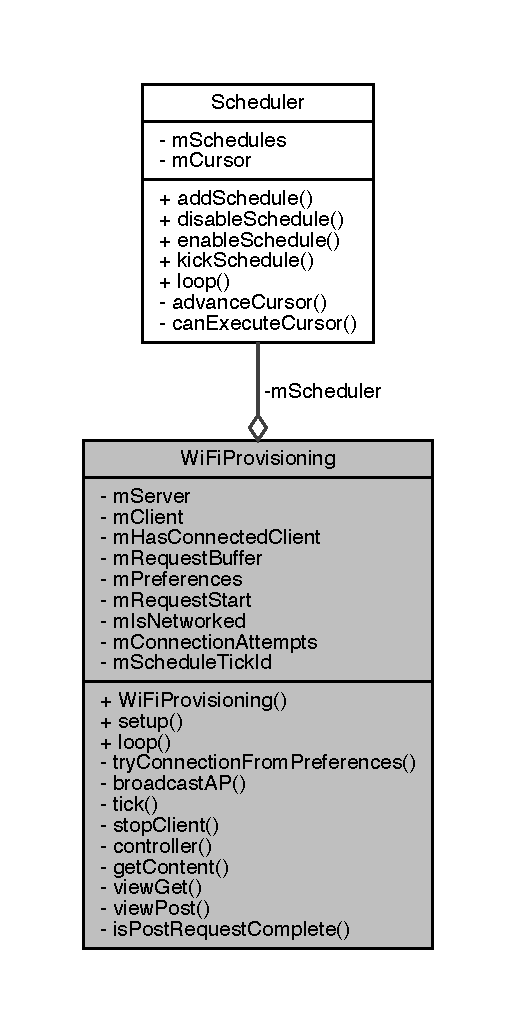
\includegraphics[width=248pt]{class_wi_fi_provisioning__coll__graph}
\end{center}
\end{figure}
\subsection*{Public Member Functions}
\begin{DoxyCompactItemize}
\item 
\mbox{\hyperlink{class_wi_fi_provisioning_afbbef380855199c9b26fbd8c57c3b6e1}{Wi\+Fi\+Provisioning}} ()
\item 
void \mbox{\hyperlink{class_wi_fi_provisioning_a82297da1523e801f8173337091bb72ee}{setup}} ()
\item 
void \mbox{\hyperlink{class_wi_fi_provisioning_afe176c8aa10c718471ea8608d335d1c4}{loop}} ()
\end{DoxyCompactItemize}
\subsection*{Private Member Functions}
\begin{DoxyCompactItemize}
\item 
bool \mbox{\hyperlink{class_wi_fi_provisioning_a407f25abd209fbadc4385b02ea9cf7ed}{try\+Connection\+From\+Preferences}} ()
\item 
void \mbox{\hyperlink{class_wi_fi_provisioning_ab117eb89658dbbaebf6b940ef2fbf66c}{broadcast\+AP}} ()
\item 
void \mbox{\hyperlink{class_wi_fi_provisioning_a6ab4c333ef20388b336310bcd7edec6a}{tick}} ()
\item 
void \mbox{\hyperlink{class_wi_fi_provisioning_a482d01497b2e4319c427658dd036a5a9}{stop\+Client}} ()
\item 
void \mbox{\hyperlink{class_wi_fi_provisioning_a6cb7ce7ff15da1fefee419e33a43459c}{controller}} ()
\item 
std\+::string \mbox{\hyperlink{class_wi_fi_provisioning_ae3cfba93792f975df0bddf6328330d68}{get\+Content}} ()
\item 
void \mbox{\hyperlink{class_wi_fi_provisioning_a3d0b39ab0ec9cf3260e82d19c471d0fe}{view\+Get}} ()
\item 
void \mbox{\hyperlink{class_wi_fi_provisioning_ac27fd34f6f6dd317f2fba2d4bb7e609e}{view\+Post}} ()
\item 
bool \mbox{\hyperlink{class_wi_fi_provisioning_abab0aebc8cca7590962e6e513010fb43}{is\+Post\+Request\+Complete}} ()
\end{DoxyCompactItemize}
\subsection*{Private Attributes}
\begin{DoxyCompactItemize}
\item 
Wi\+Fi\+Server \mbox{\hyperlink{class_wi_fi_provisioning_a88e571f1efd1e428e43209112b8c7171}{m\+Server}}
\item 
Wi\+Fi\+Client \mbox{\hyperlink{class_wi_fi_provisioning_a1a54c3ca59fb3c3cc9c0762a90ac19b8}{m\+Client}}
\item 
bool \mbox{\hyperlink{class_wi_fi_provisioning_a48db3ee3b21d4fa713871b0dda70aa8b}{m\+Has\+Connected\+Client}}
\item 
std\+::string \mbox{\hyperlink{class_wi_fi_provisioning_a1f5a015d51939cb267c52cf8e2343925}{m\+Request\+Buffer}}
\item 
Preferences \mbox{\hyperlink{class_wi_fi_provisioning_a7008915e029e3ccaa96d3a90cb54b23f}{m\+Preferences}}
\item 
size\+\_\+t \mbox{\hyperlink{class_wi_fi_provisioning_ac1a07586d838aaba494f632fbc860720}{m\+Request\+Start}}
\item 
bool \mbox{\hyperlink{class_wi_fi_provisioning_a4866e3ed981a3c39bd68019704e19334}{m\+Is\+Networked}}
\item 
uint8\+\_\+t \mbox{\hyperlink{class_wi_fi_provisioning_a9dbf21d2662da425ce4e5fc04f25baac}{m\+Connection\+Attempts}}
\item 
\mbox{\hyperlink{class_scheduler}{Scheduler}} \mbox{\hyperlink{class_wi_fi_provisioning_a526e09058cb137d8b5b05830584317d8}{m\+Scheduler}}
\item 
\mbox{\hyperlink{_scheduler_8h_a1e3b4605bdcbb8f6df7c47013e26e910}{Schedule\+Id}} \mbox{\hyperlink{class_wi_fi_provisioning_a53fd157ea3bae357292188eba8dc81b6}{m\+Schedule\+Tick\+Id}}
\end{DoxyCompactItemize}


\subsection{Detailed Description}
Manages the web application for provisioning connectivity information. 

Responsiblities\+: \begin{DoxyVerb}- Connecting to an SSID if one has been stored in Flash memory
  (Preferences).
- Broadcasting an AP if a network cannot be successfully connected to.
- Serving a webpage that allows configuration of WiFi and MQTT
  parameters.
- Writing Preferences to Flash memory.\end{DoxyVerb}
 

\subsection{Constructor \& Destructor Documentation}
\mbox{\Hypertarget{class_wi_fi_provisioning_afbbef380855199c9b26fbd8c57c3b6e1}\label{class_wi_fi_provisioning_afbbef380855199c9b26fbd8c57c3b6e1}} 
\index{Wi\+Fi\+Provisioning@{Wi\+Fi\+Provisioning}!Wi\+Fi\+Provisioning@{Wi\+Fi\+Provisioning}}
\index{Wi\+Fi\+Provisioning@{Wi\+Fi\+Provisioning}!Wi\+Fi\+Provisioning@{Wi\+Fi\+Provisioning}}
\subsubsection{\texorpdfstring{Wi\+Fi\+Provisioning()}{WiFiProvisioning()}}
{\footnotesize\ttfamily Wi\+Fi\+Provisioning\+::\+Wi\+Fi\+Provisioning (\begin{DoxyParamCaption}{ }\end{DoxyParamCaption})}



\subsection{Member Function Documentation}
\mbox{\Hypertarget{class_wi_fi_provisioning_ab117eb89658dbbaebf6b940ef2fbf66c}\label{class_wi_fi_provisioning_ab117eb89658dbbaebf6b940ef2fbf66c}} 
\index{Wi\+Fi\+Provisioning@{Wi\+Fi\+Provisioning}!broadcast\+AP@{broadcast\+AP}}
\index{broadcast\+AP@{broadcast\+AP}!Wi\+Fi\+Provisioning@{Wi\+Fi\+Provisioning}}
\subsubsection{\texorpdfstring{broadcast\+A\+P()}{broadcastAP()}}
{\footnotesize\ttfamily void Wi\+Fi\+Provisioning\+::broadcast\+AP (\begin{DoxyParamCaption}{ }\end{DoxyParamCaption})\hspace{0.3cm}{\ttfamily [private]}}

\mbox{\Hypertarget{class_wi_fi_provisioning_a6cb7ce7ff15da1fefee419e33a43459c}\label{class_wi_fi_provisioning_a6cb7ce7ff15da1fefee419e33a43459c}} 
\index{Wi\+Fi\+Provisioning@{Wi\+Fi\+Provisioning}!controller@{controller}}
\index{controller@{controller}!Wi\+Fi\+Provisioning@{Wi\+Fi\+Provisioning}}
\subsubsection{\texorpdfstring{controller()}{controller()}}
{\footnotesize\ttfamily void Wi\+Fi\+Provisioning\+::controller (\begin{DoxyParamCaption}{ }\end{DoxyParamCaption})\hspace{0.3cm}{\ttfamily [private]}}

\mbox{[}Web Server\mbox{]} Parse an incoming request and dispatch to either the G\+ET or P\+O\+ST view if we\textquotesingle{}ve received a complete request. \mbox{\Hypertarget{class_wi_fi_provisioning_ae3cfba93792f975df0bddf6328330d68}\label{class_wi_fi_provisioning_ae3cfba93792f975df0bddf6328330d68}} 
\index{Wi\+Fi\+Provisioning@{Wi\+Fi\+Provisioning}!get\+Content@{get\+Content}}
\index{get\+Content@{get\+Content}!Wi\+Fi\+Provisioning@{Wi\+Fi\+Provisioning}}
\subsubsection{\texorpdfstring{get\+Content()}{getContent()}}
{\footnotesize\ttfamily std\+::string Wi\+Fi\+Provisioning\+::get\+Content (\begin{DoxyParamCaption}{ }\end{DoxyParamCaption})\hspace{0.3cm}{\ttfamily [private]}}

\mbox{[}Web Server\mbox{]} Get the form page and populate default values from Flash memory. \mbox{\Hypertarget{class_wi_fi_provisioning_abab0aebc8cca7590962e6e513010fb43}\label{class_wi_fi_provisioning_abab0aebc8cca7590962e6e513010fb43}} 
\index{Wi\+Fi\+Provisioning@{Wi\+Fi\+Provisioning}!is\+Post\+Request\+Complete@{is\+Post\+Request\+Complete}}
\index{is\+Post\+Request\+Complete@{is\+Post\+Request\+Complete}!Wi\+Fi\+Provisioning@{Wi\+Fi\+Provisioning}}
\subsubsection{\texorpdfstring{is\+Post\+Request\+Complete()}{isPostRequestComplete()}}
{\footnotesize\ttfamily bool Wi\+Fi\+Provisioning\+::is\+Post\+Request\+Complete (\begin{DoxyParamCaption}{ }\end{DoxyParamCaption})\hspace{0.3cm}{\ttfamily [private]}}

\mbox{[}Web Server\mbox{]} Determine if we\textquotesingle{}ve received Content-\/\+Length amount of payload. \mbox{\Hypertarget{class_wi_fi_provisioning_afe176c8aa10c718471ea8608d335d1c4}\label{class_wi_fi_provisioning_afe176c8aa10c718471ea8608d335d1c4}} 
\index{Wi\+Fi\+Provisioning@{Wi\+Fi\+Provisioning}!loop@{loop}}
\index{loop@{loop}!Wi\+Fi\+Provisioning@{Wi\+Fi\+Provisioning}}
\subsubsection{\texorpdfstring{loop()}{loop()}}
{\footnotesize\ttfamily void Wi\+Fi\+Provisioning\+::loop (\begin{DoxyParamCaption}{ }\end{DoxyParamCaption})}

\mbox{\Hypertarget{class_wi_fi_provisioning_a82297da1523e801f8173337091bb72ee}\label{class_wi_fi_provisioning_a82297da1523e801f8173337091bb72ee}} 
\index{Wi\+Fi\+Provisioning@{Wi\+Fi\+Provisioning}!setup@{setup}}
\index{setup@{setup}!Wi\+Fi\+Provisioning@{Wi\+Fi\+Provisioning}}
\subsubsection{\texorpdfstring{setup()}{setup()}}
{\footnotesize\ttfamily void Wi\+Fi\+Provisioning\+::setup (\begin{DoxyParamCaption}{ }\end{DoxyParamCaption})}

\mbox{\Hypertarget{class_wi_fi_provisioning_a482d01497b2e4319c427658dd036a5a9}\label{class_wi_fi_provisioning_a482d01497b2e4319c427658dd036a5a9}} 
\index{Wi\+Fi\+Provisioning@{Wi\+Fi\+Provisioning}!stop\+Client@{stop\+Client}}
\index{stop\+Client@{stop\+Client}!Wi\+Fi\+Provisioning@{Wi\+Fi\+Provisioning}}
\subsubsection{\texorpdfstring{stop\+Client()}{stopClient()}}
{\footnotesize\ttfamily void Wi\+Fi\+Provisioning\+::stop\+Client (\begin{DoxyParamCaption}{ }\end{DoxyParamCaption})\hspace{0.3cm}{\ttfamily [private]}}

\mbox{[}Web Server\mbox{]} \mbox{\Hypertarget{class_wi_fi_provisioning_a6ab4c333ef20388b336310bcd7edec6a}\label{class_wi_fi_provisioning_a6ab4c333ef20388b336310bcd7edec6a}} 
\index{Wi\+Fi\+Provisioning@{Wi\+Fi\+Provisioning}!tick@{tick}}
\index{tick@{tick}!Wi\+Fi\+Provisioning@{Wi\+Fi\+Provisioning}}
\subsubsection{\texorpdfstring{tick()}{tick()}}
{\footnotesize\ttfamily void Wi\+Fi\+Provisioning\+::tick (\begin{DoxyParamCaption}{ }\end{DoxyParamCaption})\hspace{0.3cm}{\ttfamily [private]}}

Check to see if we\textquotesingle{}re connected yet. If we exceed the connection attempts then we should bail and just broadcast an AP. \mbox{\Hypertarget{class_wi_fi_provisioning_a407f25abd209fbadc4385b02ea9cf7ed}\label{class_wi_fi_provisioning_a407f25abd209fbadc4385b02ea9cf7ed}} 
\index{Wi\+Fi\+Provisioning@{Wi\+Fi\+Provisioning}!try\+Connection\+From\+Preferences@{try\+Connection\+From\+Preferences}}
\index{try\+Connection\+From\+Preferences@{try\+Connection\+From\+Preferences}!Wi\+Fi\+Provisioning@{Wi\+Fi\+Provisioning}}
\subsubsection{\texorpdfstring{try\+Connection\+From\+Preferences()}{tryConnectionFromPreferences()}}
{\footnotesize\ttfamily bool Wi\+Fi\+Provisioning\+::try\+Connection\+From\+Preferences (\begin{DoxyParamCaption}{ }\end{DoxyParamCaption})\hspace{0.3cm}{\ttfamily [private]}}

Returns false if S\+S\+ID and password are not set. \mbox{\Hypertarget{class_wi_fi_provisioning_a3d0b39ab0ec9cf3260e82d19c471d0fe}\label{class_wi_fi_provisioning_a3d0b39ab0ec9cf3260e82d19c471d0fe}} 
\index{Wi\+Fi\+Provisioning@{Wi\+Fi\+Provisioning}!view\+Get@{view\+Get}}
\index{view\+Get@{view\+Get}!Wi\+Fi\+Provisioning@{Wi\+Fi\+Provisioning}}
\subsubsection{\texorpdfstring{view\+Get()}{viewGet()}}
{\footnotesize\ttfamily void Wi\+Fi\+Provisioning\+::view\+Get (\begin{DoxyParamCaption}{ }\end{DoxyParamCaption})\hspace{0.3cm}{\ttfamily [private]}}

\mbox{[}Web Server\mbox{]} \mbox{\Hypertarget{class_wi_fi_provisioning_ac27fd34f6f6dd317f2fba2d4bb7e609e}\label{class_wi_fi_provisioning_ac27fd34f6f6dd317f2fba2d4bb7e609e}} 
\index{Wi\+Fi\+Provisioning@{Wi\+Fi\+Provisioning}!view\+Post@{view\+Post}}
\index{view\+Post@{view\+Post}!Wi\+Fi\+Provisioning@{Wi\+Fi\+Provisioning}}
\subsubsection{\texorpdfstring{view\+Post()}{viewPost()}}
{\footnotesize\ttfamily void Wi\+Fi\+Provisioning\+::view\+Post (\begin{DoxyParamCaption}{ }\end{DoxyParamCaption})\hspace{0.3cm}{\ttfamily [private]}}

\mbox{[}Web Server\mbox{]} 

\subsection{Member Data Documentation}
\mbox{\Hypertarget{class_wi_fi_provisioning_a1a54c3ca59fb3c3cc9c0762a90ac19b8}\label{class_wi_fi_provisioning_a1a54c3ca59fb3c3cc9c0762a90ac19b8}} 
\index{Wi\+Fi\+Provisioning@{Wi\+Fi\+Provisioning}!m\+Client@{m\+Client}}
\index{m\+Client@{m\+Client}!Wi\+Fi\+Provisioning@{Wi\+Fi\+Provisioning}}
\subsubsection{\texorpdfstring{m\+Client}{mClient}}
{\footnotesize\ttfamily Wi\+Fi\+Client Wi\+Fi\+Provisioning\+::m\+Client\hspace{0.3cm}{\ttfamily [private]}}

\mbox{\Hypertarget{class_wi_fi_provisioning_a9dbf21d2662da425ce4e5fc04f25baac}\label{class_wi_fi_provisioning_a9dbf21d2662da425ce4e5fc04f25baac}} 
\index{Wi\+Fi\+Provisioning@{Wi\+Fi\+Provisioning}!m\+Connection\+Attempts@{m\+Connection\+Attempts}}
\index{m\+Connection\+Attempts@{m\+Connection\+Attempts}!Wi\+Fi\+Provisioning@{Wi\+Fi\+Provisioning}}
\subsubsection{\texorpdfstring{m\+Connection\+Attempts}{mConnectionAttempts}}
{\footnotesize\ttfamily uint8\+\_\+t Wi\+Fi\+Provisioning\+::m\+Connection\+Attempts\hspace{0.3cm}{\ttfamily [private]}}

\mbox{\Hypertarget{class_wi_fi_provisioning_a48db3ee3b21d4fa713871b0dda70aa8b}\label{class_wi_fi_provisioning_a48db3ee3b21d4fa713871b0dda70aa8b}} 
\index{Wi\+Fi\+Provisioning@{Wi\+Fi\+Provisioning}!m\+Has\+Connected\+Client@{m\+Has\+Connected\+Client}}
\index{m\+Has\+Connected\+Client@{m\+Has\+Connected\+Client}!Wi\+Fi\+Provisioning@{Wi\+Fi\+Provisioning}}
\subsubsection{\texorpdfstring{m\+Has\+Connected\+Client}{mHasConnectedClient}}
{\footnotesize\ttfamily bool Wi\+Fi\+Provisioning\+::m\+Has\+Connected\+Client\hspace{0.3cm}{\ttfamily [private]}}

\mbox{\Hypertarget{class_wi_fi_provisioning_a4866e3ed981a3c39bd68019704e19334}\label{class_wi_fi_provisioning_a4866e3ed981a3c39bd68019704e19334}} 
\index{Wi\+Fi\+Provisioning@{Wi\+Fi\+Provisioning}!m\+Is\+Networked@{m\+Is\+Networked}}
\index{m\+Is\+Networked@{m\+Is\+Networked}!Wi\+Fi\+Provisioning@{Wi\+Fi\+Provisioning}}
\subsubsection{\texorpdfstring{m\+Is\+Networked}{mIsNetworked}}
{\footnotesize\ttfamily bool Wi\+Fi\+Provisioning\+::m\+Is\+Networked\hspace{0.3cm}{\ttfamily [private]}}

Are we connected to a network or broadcasting an AP? \mbox{\Hypertarget{class_wi_fi_provisioning_a7008915e029e3ccaa96d3a90cb54b23f}\label{class_wi_fi_provisioning_a7008915e029e3ccaa96d3a90cb54b23f}} 
\index{Wi\+Fi\+Provisioning@{Wi\+Fi\+Provisioning}!m\+Preferences@{m\+Preferences}}
\index{m\+Preferences@{m\+Preferences}!Wi\+Fi\+Provisioning@{Wi\+Fi\+Provisioning}}
\subsubsection{\texorpdfstring{m\+Preferences}{mPreferences}}
{\footnotesize\ttfamily Preferences Wi\+Fi\+Provisioning\+::m\+Preferences\hspace{0.3cm}{\ttfamily [private]}}

\mbox{\Hypertarget{class_wi_fi_provisioning_a1f5a015d51939cb267c52cf8e2343925}\label{class_wi_fi_provisioning_a1f5a015d51939cb267c52cf8e2343925}} 
\index{Wi\+Fi\+Provisioning@{Wi\+Fi\+Provisioning}!m\+Request\+Buffer@{m\+Request\+Buffer}}
\index{m\+Request\+Buffer@{m\+Request\+Buffer}!Wi\+Fi\+Provisioning@{Wi\+Fi\+Provisioning}}
\subsubsection{\texorpdfstring{m\+Request\+Buffer}{mRequestBuffer}}
{\footnotesize\ttfamily std\+::string Wi\+Fi\+Provisioning\+::m\+Request\+Buffer\hspace{0.3cm}{\ttfamily [private]}}

\mbox{\Hypertarget{class_wi_fi_provisioning_ac1a07586d838aaba494f632fbc860720}\label{class_wi_fi_provisioning_ac1a07586d838aaba494f632fbc860720}} 
\index{Wi\+Fi\+Provisioning@{Wi\+Fi\+Provisioning}!m\+Request\+Start@{m\+Request\+Start}}
\index{m\+Request\+Start@{m\+Request\+Start}!Wi\+Fi\+Provisioning@{Wi\+Fi\+Provisioning}}
\subsubsection{\texorpdfstring{m\+Request\+Start}{mRequestStart}}
{\footnotesize\ttfamily size\+\_\+t Wi\+Fi\+Provisioning\+::m\+Request\+Start\hspace{0.3cm}{\ttfamily [private]}}

Allow us to timeout a H\+T\+TP request. \mbox{\Hypertarget{class_wi_fi_provisioning_a526e09058cb137d8b5b05830584317d8}\label{class_wi_fi_provisioning_a526e09058cb137d8b5b05830584317d8}} 
\index{Wi\+Fi\+Provisioning@{Wi\+Fi\+Provisioning}!m\+Scheduler@{m\+Scheduler}}
\index{m\+Scheduler@{m\+Scheduler}!Wi\+Fi\+Provisioning@{Wi\+Fi\+Provisioning}}
\subsubsection{\texorpdfstring{m\+Scheduler}{mScheduler}}
{\footnotesize\ttfamily \mbox{\hyperlink{class_scheduler}{Scheduler}} Wi\+Fi\+Provisioning\+::m\+Scheduler\hspace{0.3cm}{\ttfamily [private]}}

\mbox{\Hypertarget{class_wi_fi_provisioning_a53fd157ea3bae357292188eba8dc81b6}\label{class_wi_fi_provisioning_a53fd157ea3bae357292188eba8dc81b6}} 
\index{Wi\+Fi\+Provisioning@{Wi\+Fi\+Provisioning}!m\+Schedule\+Tick\+Id@{m\+Schedule\+Tick\+Id}}
\index{m\+Schedule\+Tick\+Id@{m\+Schedule\+Tick\+Id}!Wi\+Fi\+Provisioning@{Wi\+Fi\+Provisioning}}
\subsubsection{\texorpdfstring{m\+Schedule\+Tick\+Id}{mScheduleTickId}}
{\footnotesize\ttfamily \mbox{\hyperlink{_scheduler_8h_a1e3b4605bdcbb8f6df7c47013e26e910}{Schedule\+Id}} Wi\+Fi\+Provisioning\+::m\+Schedule\+Tick\+Id\hspace{0.3cm}{\ttfamily [private]}}

\mbox{\Hypertarget{class_wi_fi_provisioning_a88e571f1efd1e428e43209112b8c7171}\label{class_wi_fi_provisioning_a88e571f1efd1e428e43209112b8c7171}} 
\index{Wi\+Fi\+Provisioning@{Wi\+Fi\+Provisioning}!m\+Server@{m\+Server}}
\index{m\+Server@{m\+Server}!Wi\+Fi\+Provisioning@{Wi\+Fi\+Provisioning}}
\subsubsection{\texorpdfstring{m\+Server}{mServer}}
{\footnotesize\ttfamily Wi\+Fi\+Server Wi\+Fi\+Provisioning\+::m\+Server\hspace{0.3cm}{\ttfamily [private]}}



The documentation for this class was generated from the following files\+:\begin{DoxyCompactItemize}
\item 
include/\mbox{\hyperlink{_wi_fi_provisioning_8h}{Wi\+Fi\+Provisioning.\+h}}\item 
src/\mbox{\hyperlink{_wi_fi_provisioning_8cpp}{Wi\+Fi\+Provisioning.\+cpp}}\end{DoxyCompactItemize}

\chapter{File Documentation}
\hypertarget{_i2_c_manager_8h}{}\section{include/\+I2\+C\+Manager.h File Reference}
\label{_i2_c_manager_8h}\index{include/\+I2\+C\+Manager.\+h@{include/\+I2\+C\+Manager.\+h}}
{\ttfamily \#include $<$bitset$>$}\newline
{\ttfamily \#include $<$Wire.\+h$>$}\newline
{\ttfamily \#include \char`\"{}Scheduler.\+h\char`\"{}}\newline
Include dependency graph for I2\+C\+Manager.\+h\+:\nopagebreak
\begin{figure}[H]
\begin{center}
\leavevmode
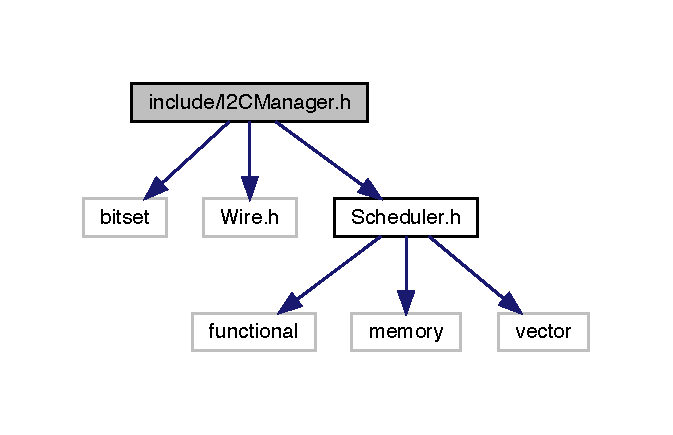
\includegraphics[width=323pt]{_i2_c_manager_8h__incl}
\end{center}
\end{figure}
This graph shows which files directly or indirectly include this file\+:\nopagebreak
\begin{figure}[H]
\begin{center}
\leavevmode
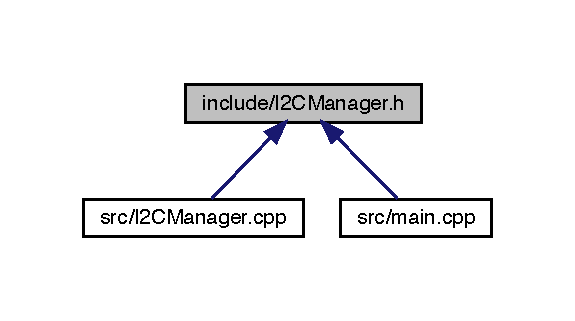
\includegraphics[width=276pt]{_i2_c_manager_8h__dep__incl}
\end{center}
\end{figure}
\subsection*{Classes}
\begin{DoxyCompactItemize}
\item 
class \mbox{\hyperlink{class_i2_c_manager}{I2\+C\+Manager}}
\begin{DoxyCompactList}\small\item\em Responsible for discovering the connectivity status of I2C peripherals. \end{DoxyCompactList}\end{DoxyCompactItemize}
\subsection*{Macros}
\begin{DoxyCompactItemize}
\item 
\#define \mbox{\hyperlink{_i2_c_manager_8h_a5aa8afc0ad4792d13a6cb089c9d50537}{I2\+C\+M\+A\+N\+A\+G\+E\+R\+\_\+\+D\+E\+F\+A\+U\+L\+T\+\_\+\+I\+N\+T\+E\+R\+\_\+\+S\+C\+A\+N\+\_\+\+P\+E\+R\+I\+OD}}~1000
\item 
\#define \mbox{\hyperlink{_i2_c_manager_8h_a9b3d76aae3ebcca37db7e5d8cae3053e}{I2\+C\+M\+A\+N\+A\+G\+E\+R\+\_\+\+D\+E\+F\+A\+U\+L\+T\+\_\+\+I\+N\+T\+R\+A\+\_\+\+S\+C\+A\+N\+\_\+\+P\+E\+R\+I\+OD}}~10
\end{DoxyCompactItemize}


\subsection{Macro Definition Documentation}
\mbox{\Hypertarget{_i2_c_manager_8h_a5aa8afc0ad4792d13a6cb089c9d50537}\label{_i2_c_manager_8h_a5aa8afc0ad4792d13a6cb089c9d50537}} 
\index{I2\+C\+Manager.\+h@{I2\+C\+Manager.\+h}!I2\+C\+M\+A\+N\+A\+G\+E\+R\+\_\+\+D\+E\+F\+A\+U\+L\+T\+\_\+\+I\+N\+T\+E\+R\+\_\+\+S\+C\+A\+N\+\_\+\+P\+E\+R\+I\+OD@{I2\+C\+M\+A\+N\+A\+G\+E\+R\+\_\+\+D\+E\+F\+A\+U\+L\+T\+\_\+\+I\+N\+T\+E\+R\+\_\+\+S\+C\+A\+N\+\_\+\+P\+E\+R\+I\+OD}}
\index{I2\+C\+M\+A\+N\+A\+G\+E\+R\+\_\+\+D\+E\+F\+A\+U\+L\+T\+\_\+\+I\+N\+T\+E\+R\+\_\+\+S\+C\+A\+N\+\_\+\+P\+E\+R\+I\+OD@{I2\+C\+M\+A\+N\+A\+G\+E\+R\+\_\+\+D\+E\+F\+A\+U\+L\+T\+\_\+\+I\+N\+T\+E\+R\+\_\+\+S\+C\+A\+N\+\_\+\+P\+E\+R\+I\+OD}!I2\+C\+Manager.\+h@{I2\+C\+Manager.\+h}}
\subsubsection{\texorpdfstring{I2\+C\+M\+A\+N\+A\+G\+E\+R\+\_\+\+D\+E\+F\+A\+U\+L\+T\+\_\+\+I\+N\+T\+E\+R\+\_\+\+S\+C\+A\+N\+\_\+\+P\+E\+R\+I\+OD}{I2CMANAGER\_DEFAULT\_INTER\_SCAN\_PERIOD}}
{\footnotesize\ttfamily \#define I2\+C\+M\+A\+N\+A\+G\+E\+R\+\_\+\+D\+E\+F\+A\+U\+L\+T\+\_\+\+I\+N\+T\+E\+R\+\_\+\+S\+C\+A\+N\+\_\+\+P\+E\+R\+I\+OD~1000}

\mbox{\Hypertarget{_i2_c_manager_8h_a9b3d76aae3ebcca37db7e5d8cae3053e}\label{_i2_c_manager_8h_a9b3d76aae3ebcca37db7e5d8cae3053e}} 
\index{I2\+C\+Manager.\+h@{I2\+C\+Manager.\+h}!I2\+C\+M\+A\+N\+A\+G\+E\+R\+\_\+\+D\+E\+F\+A\+U\+L\+T\+\_\+\+I\+N\+T\+R\+A\+\_\+\+S\+C\+A\+N\+\_\+\+P\+E\+R\+I\+OD@{I2\+C\+M\+A\+N\+A\+G\+E\+R\+\_\+\+D\+E\+F\+A\+U\+L\+T\+\_\+\+I\+N\+T\+R\+A\+\_\+\+S\+C\+A\+N\+\_\+\+P\+E\+R\+I\+OD}}
\index{I2\+C\+M\+A\+N\+A\+G\+E\+R\+\_\+\+D\+E\+F\+A\+U\+L\+T\+\_\+\+I\+N\+T\+R\+A\+\_\+\+S\+C\+A\+N\+\_\+\+P\+E\+R\+I\+OD@{I2\+C\+M\+A\+N\+A\+G\+E\+R\+\_\+\+D\+E\+F\+A\+U\+L\+T\+\_\+\+I\+N\+T\+R\+A\+\_\+\+S\+C\+A\+N\+\_\+\+P\+E\+R\+I\+OD}!I2\+C\+Manager.\+h@{I2\+C\+Manager.\+h}}
\subsubsection{\texorpdfstring{I2\+C\+M\+A\+N\+A\+G\+E\+R\+\_\+\+D\+E\+F\+A\+U\+L\+T\+\_\+\+I\+N\+T\+R\+A\+\_\+\+S\+C\+A\+N\+\_\+\+P\+E\+R\+I\+OD}{I2CMANAGER\_DEFAULT\_INTRA\_SCAN\_PERIOD}}
{\footnotesize\ttfamily \#define I2\+C\+M\+A\+N\+A\+G\+E\+R\+\_\+\+D\+E\+F\+A\+U\+L\+T\+\_\+\+I\+N\+T\+R\+A\+\_\+\+S\+C\+A\+N\+\_\+\+P\+E\+R\+I\+OD~10}


\hypertarget{_i2_c_peripheral_8h}{}\section{include/\+I2\+C\+Peripheral.h File Reference}
\label{_i2_c_peripheral_8h}\index{include/\+I2\+C\+Peripheral.\+h@{include/\+I2\+C\+Peripheral.\+h}}
{\ttfamily \#include \char`\"{}Scheduler.\+h\char`\"{}}\newline
Include dependency graph for I2\+C\+Peripheral.\+h\+:\nopagebreak
\begin{figure}[H]
\begin{center}
\leavevmode
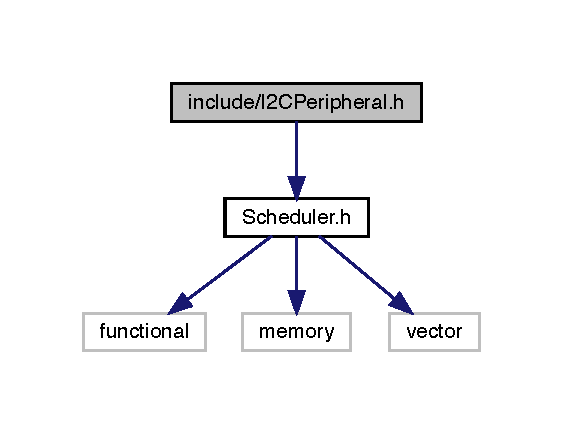
\includegraphics[width=270pt]{_i2_c_peripheral_8h__incl}
\end{center}
\end{figure}
This graph shows which files directly or indirectly include this file\+:\nopagebreak
\begin{figure}[H]
\begin{center}
\leavevmode
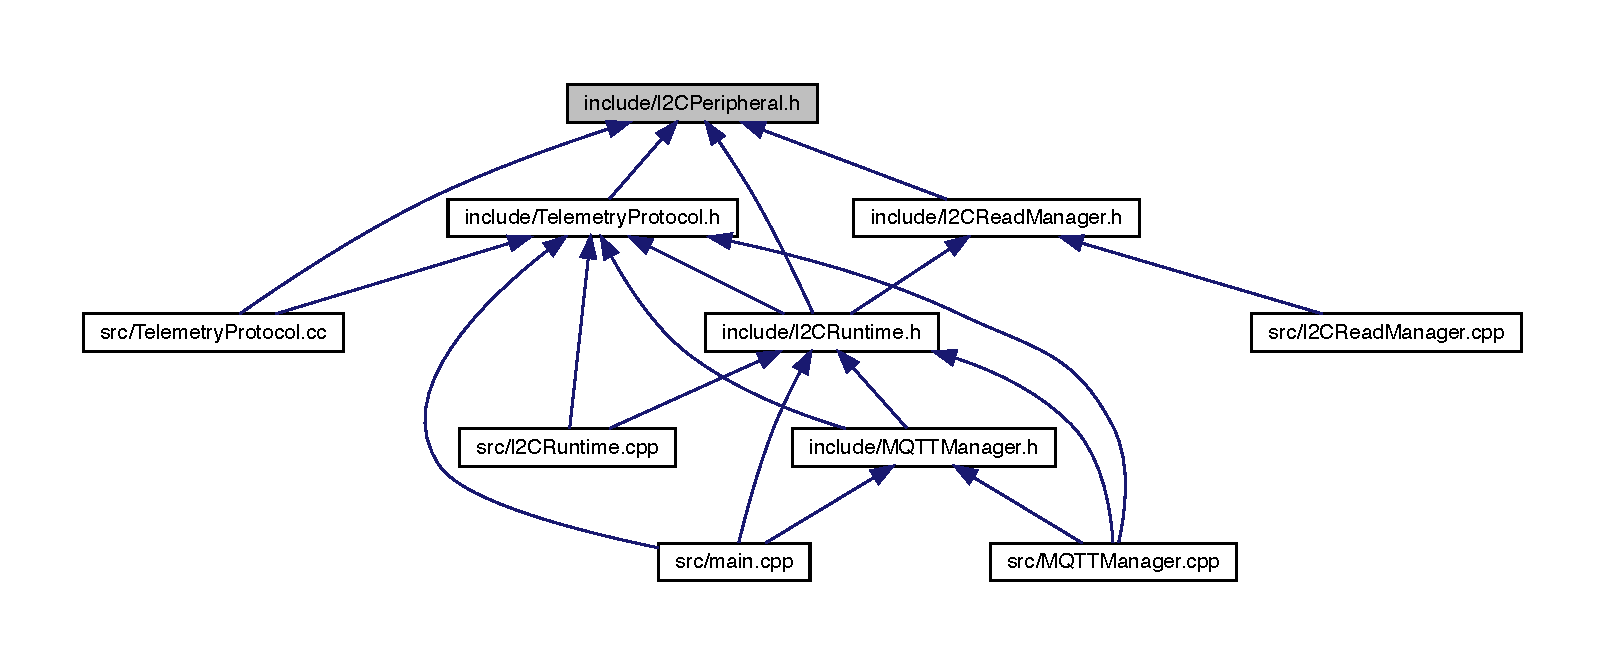
\includegraphics[width=350pt]{_i2_c_peripheral_8h__dep__incl}
\end{center}
\end{figure}
\subsection*{Classes}
\begin{DoxyCompactItemize}
\item 
struct \mbox{\hyperlink{struct_read_definition}{Read\+Definition}}
\begin{DoxyCompactList}\small\item\em Declarative configuration for reading a contiguous register block from a peripheral on the I2C bus. \end{DoxyCompactList}\item 
struct \mbox{\hyperlink{struct_setup_write_definition}{Setup\+Write\+Definition}}
\item 
struct \mbox{\hyperlink{struct_peripheral}{Peripheral}}
\begin{DoxyCompactList}\small\item\em Declarative configuration for the behaviour of a peripheral on the I2C bus. \end{DoxyCompactList}\end{DoxyCompactItemize}
\subsection*{Macros}
\begin{DoxyCompactItemize}
\item 
\#define \mbox{\hyperlink{_i2_c_peripheral_8h_a844808a972fe52f905460a2e611f96af}{R\+E\+G\+I\+S\+T\+E\+R\+\_\+\+R\+E\+Q\+\_\+\+D\+E\+L\+A\+Y\+\_\+\+M\+I\+L\+LI}}~15
\end{DoxyCompactItemize}
\subsection*{Typedefs}
\begin{DoxyCompactItemize}
\item 
typedef struct \mbox{\hyperlink{struct_read_definition}{Read\+Definition}} \mbox{\hyperlink{_i2_c_peripheral_8h_ae09d4fb5ac84b480bc5f785562e0bc3b}{Read\+Definition}}
\item 
typedef struct \mbox{\hyperlink{struct_setup_write_definition}{Setup\+Write\+Definition}} \mbox{\hyperlink{_i2_c_peripheral_8h_aedb5e72c14b49628073e1d0c881d850b}{Setup\+Write\+Definition}}
\item 
typedef struct \mbox{\hyperlink{struct_peripheral}{Peripheral}} \mbox{\hyperlink{_i2_c_peripheral_8h_adb61d3f4d9c37b38b0746b9fa539a1c3}{Peripheral}}
\end{DoxyCompactItemize}
\subsection*{Enumerations}
\begin{DoxyCompactItemize}
\item 
enum \mbox{\hyperlink{_i2_c_peripheral_8h_ae0efcb4a72d88c76f03e57ed26b03383}{Register\+Length}} \{ \mbox{\hyperlink{_i2_c_peripheral_8h_ae0efcb4a72d88c76f03e57ed26b03383ae0e4fac35509ec53d2e8aecb33f3cb45}{R\+L16}}, 
\mbox{\hyperlink{_i2_c_peripheral_8h_ae0efcb4a72d88c76f03e57ed26b03383ac2c6b7ffba3b85b1a4990575466fc484}{R\+L8}}
 \}
\end{DoxyCompactItemize}


\subsection{Macro Definition Documentation}
\mbox{\Hypertarget{_i2_c_peripheral_8h_a844808a972fe52f905460a2e611f96af}\label{_i2_c_peripheral_8h_a844808a972fe52f905460a2e611f96af}} 
\index{I2\+C\+Peripheral.\+h@{I2\+C\+Peripheral.\+h}!R\+E\+G\+I\+S\+T\+E\+R\+\_\+\+R\+E\+Q\+\_\+\+D\+E\+L\+A\+Y\+\_\+\+M\+I\+L\+LI@{R\+E\+G\+I\+S\+T\+E\+R\+\_\+\+R\+E\+Q\+\_\+\+D\+E\+L\+A\+Y\+\_\+\+M\+I\+L\+LI}}
\index{R\+E\+G\+I\+S\+T\+E\+R\+\_\+\+R\+E\+Q\+\_\+\+D\+E\+L\+A\+Y\+\_\+\+M\+I\+L\+LI@{R\+E\+G\+I\+S\+T\+E\+R\+\_\+\+R\+E\+Q\+\_\+\+D\+E\+L\+A\+Y\+\_\+\+M\+I\+L\+LI}!I2\+C\+Peripheral.\+h@{I2\+C\+Peripheral.\+h}}
\subsubsection{\texorpdfstring{R\+E\+G\+I\+S\+T\+E\+R\+\_\+\+R\+E\+Q\+\_\+\+D\+E\+L\+A\+Y\+\_\+\+M\+I\+L\+LI}{REGISTER\_REQ\_DELAY\_MILLI}}
{\footnotesize\ttfamily \#define R\+E\+G\+I\+S\+T\+E\+R\+\_\+\+R\+E\+Q\+\_\+\+D\+E\+L\+A\+Y\+\_\+\+M\+I\+L\+LI~15}

This value can be very important.

Too low\+: Insufficient time between the register ID transmission and a request to read bytes. No data will be read.

Too high\+: Performance will suffer for read definitions that have a long contiguous register block length. (e.\+g., something like the thermal camera that reads from 128 different registers.) 

\subsection{Typedef Documentation}
\mbox{\Hypertarget{_i2_c_peripheral_8h_adb61d3f4d9c37b38b0746b9fa539a1c3}\label{_i2_c_peripheral_8h_adb61d3f4d9c37b38b0746b9fa539a1c3}} 
\index{I2\+C\+Peripheral.\+h@{I2\+C\+Peripheral.\+h}!Peripheral@{Peripheral}}
\index{Peripheral@{Peripheral}!I2\+C\+Peripheral.\+h@{I2\+C\+Peripheral.\+h}}
\subsubsection{\texorpdfstring{Peripheral}{Peripheral}}
{\footnotesize\ttfamily typedef struct \mbox{\hyperlink{struct_peripheral}{Peripheral}} \mbox{\hyperlink{struct_peripheral}{Peripheral}}}

\mbox{\Hypertarget{_i2_c_peripheral_8h_ae09d4fb5ac84b480bc5f785562e0bc3b}\label{_i2_c_peripheral_8h_ae09d4fb5ac84b480bc5f785562e0bc3b}} 
\index{I2\+C\+Peripheral.\+h@{I2\+C\+Peripheral.\+h}!Read\+Definition@{Read\+Definition}}
\index{Read\+Definition@{Read\+Definition}!I2\+C\+Peripheral.\+h@{I2\+C\+Peripheral.\+h}}
\subsubsection{\texorpdfstring{Read\+Definition}{ReadDefinition}}
{\footnotesize\ttfamily typedef struct \mbox{\hyperlink{struct_read_definition}{Read\+Definition}} \mbox{\hyperlink{struct_read_definition}{Read\+Definition}}}

\mbox{\Hypertarget{_i2_c_peripheral_8h_aedb5e72c14b49628073e1d0c881d850b}\label{_i2_c_peripheral_8h_aedb5e72c14b49628073e1d0c881d850b}} 
\index{I2\+C\+Peripheral.\+h@{I2\+C\+Peripheral.\+h}!Setup\+Write\+Definition@{Setup\+Write\+Definition}}
\index{Setup\+Write\+Definition@{Setup\+Write\+Definition}!I2\+C\+Peripheral.\+h@{I2\+C\+Peripheral.\+h}}
\subsubsection{\texorpdfstring{Setup\+Write\+Definition}{SetupWriteDefinition}}
{\footnotesize\ttfamily typedef struct \mbox{\hyperlink{struct_setup_write_definition}{Setup\+Write\+Definition}} \mbox{\hyperlink{struct_setup_write_definition}{Setup\+Write\+Definition}}}



\subsection{Enumeration Type Documentation}
\mbox{\Hypertarget{_i2_c_peripheral_8h_ae0efcb4a72d88c76f03e57ed26b03383}\label{_i2_c_peripheral_8h_ae0efcb4a72d88c76f03e57ed26b03383}} 
\index{I2\+C\+Peripheral.\+h@{I2\+C\+Peripheral.\+h}!Register\+Length@{Register\+Length}}
\index{Register\+Length@{Register\+Length}!I2\+C\+Peripheral.\+h@{I2\+C\+Peripheral.\+h}}
\subsubsection{\texorpdfstring{Register\+Length}{RegisterLength}}
{\footnotesize\ttfamily enum \mbox{\hyperlink{_i2_c_peripheral_8h_ae0efcb4a72d88c76f03e57ed26b03383}{Register\+Length}}}

\begin{DoxyEnumFields}{Enumerator}
\raisebox{\heightof{T}}[0pt][0pt]{\index{R\+L16@{R\+L16}!I2\+C\+Peripheral.\+h@{I2\+C\+Peripheral.\+h}}\index{I2\+C\+Peripheral.\+h@{I2\+C\+Peripheral.\+h}!R\+L16@{R\+L16}}}\mbox{\Hypertarget{_i2_c_peripheral_8h_ae0efcb4a72d88c76f03e57ed26b03383ae0e4fac35509ec53d2e8aecb33f3cb45}\label{_i2_c_peripheral_8h_ae0efcb4a72d88c76f03e57ed26b03383ae0e4fac35509ec53d2e8aecb33f3cb45}} 
R\+L16&\\
\hline

\raisebox{\heightof{T}}[0pt][0pt]{\index{R\+L8@{R\+L8}!I2\+C\+Peripheral.\+h@{I2\+C\+Peripheral.\+h}}\index{I2\+C\+Peripheral.\+h@{I2\+C\+Peripheral.\+h}!R\+L8@{R\+L8}}}\mbox{\Hypertarget{_i2_c_peripheral_8h_ae0efcb4a72d88c76f03e57ed26b03383ac2c6b7ffba3b85b1a4990575466fc484}\label{_i2_c_peripheral_8h_ae0efcb4a72d88c76f03e57ed26b03383ac2c6b7ffba3b85b1a4990575466fc484}} 
R\+L8&\\
\hline

\end{DoxyEnumFields}

\hypertarget{_i2_c_read_manager_8h}{}\section{include/\+I2\+C\+Read\+Manager.h File Reference}
\label{_i2_c_read_manager_8h}\index{include/\+I2\+C\+Read\+Manager.\+h@{include/\+I2\+C\+Read\+Manager.\+h}}
{\ttfamily \#include $<$Wire.\+h$>$}\newline
{\ttfamily \#include \char`\"{}I2\+C\+Peripheral.\+h\char`\"{}}\newline
{\ttfamily \#include \char`\"{}Scheduler.\+h\char`\"{}}\newline
Include dependency graph for I2\+C\+Read\+Manager.\+h\+:\nopagebreak
\begin{figure}[H]
\begin{center}
\leavevmode
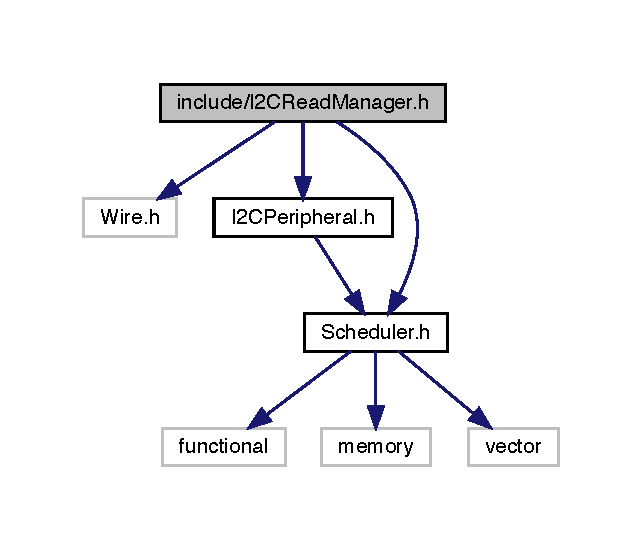
\includegraphics[width=308pt]{_i2_c_read_manager_8h__incl}
\end{center}
\end{figure}
This graph shows which files directly or indirectly include this file\+:\nopagebreak
\begin{figure}[H]
\begin{center}
\leavevmode
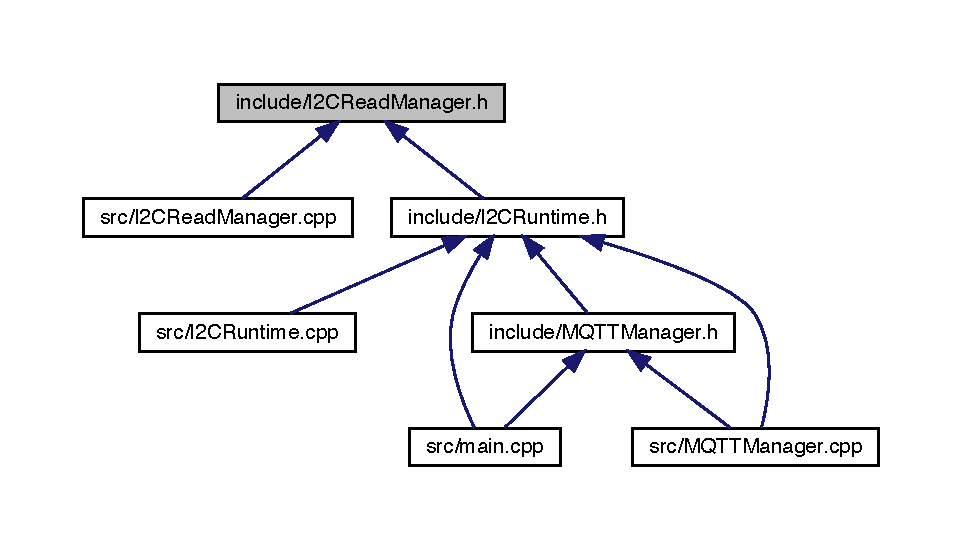
\includegraphics[width=350pt]{_i2_c_read_manager_8h__dep__incl}
\end{center}
\end{figure}
\subsection*{Classes}
\begin{DoxyCompactItemize}
\item 
class \mbox{\hyperlink{class_i2_c_read_manager}{I2\+C\+Read\+Manager}}
\begin{DoxyCompactList}\small\item\em Responsible for a state machine which reads data from the I2C bus in a non-\/blocking fashion. \end{DoxyCompactList}\end{DoxyCompactItemize}
\subsection*{Enumerations}
\begin{DoxyCompactItemize}
\item 
enum \mbox{\hyperlink{_i2_c_read_manager_8h_a6fa8ade9cf010a4fd9f7a36c4a4566aa}{Read\+Manager\+State}} \{ \mbox{\hyperlink{_i2_c_read_manager_8h_a6fa8ade9cf010a4fd9f7a36c4a4566aaae37ab7bd34b9e999f50359d981240173}{N\+O\+T\+\_\+\+R\+E\+A\+D\+I\+N\+G\+\_\+\+B\+L\+O\+CK}}, 
\mbox{\hyperlink{_i2_c_read_manager_8h_a6fa8ade9cf010a4fd9f7a36c4a4566aaa99614153608b27d690f0d91b4aed7e6b}{R\+E\+Q\+U\+E\+S\+T\+I\+N\+G\+\_\+\+S\+I\+N\+G\+L\+E\+\_\+\+R\+E\+AD}}, 
\mbox{\hyperlink{_i2_c_read_manager_8h_a6fa8ade9cf010a4fd9f7a36c4a4566aaabc3795837fd1e51d56a81344dc98a862}{R\+E\+Q\+U\+E\+S\+T\+E\+D\+\_\+\+S\+I\+N\+G\+L\+E\+\_\+\+R\+E\+AD}}
 \}
\end{DoxyCompactItemize}


\subsection{Enumeration Type Documentation}
\mbox{\Hypertarget{_i2_c_read_manager_8h_a6fa8ade9cf010a4fd9f7a36c4a4566aa}\label{_i2_c_read_manager_8h_a6fa8ade9cf010a4fd9f7a36c4a4566aa}} 
\index{I2\+C\+Read\+Manager.\+h@{I2\+C\+Read\+Manager.\+h}!Read\+Manager\+State@{Read\+Manager\+State}}
\index{Read\+Manager\+State@{Read\+Manager\+State}!I2\+C\+Read\+Manager.\+h@{I2\+C\+Read\+Manager.\+h}}
\subsubsection{\texorpdfstring{Read\+Manager\+State}{ReadManagerState}}
{\footnotesize\ttfamily enum \mbox{\hyperlink{_i2_c_read_manager_8h_a6fa8ade9cf010a4fd9f7a36c4a4566aa}{Read\+Manager\+State}}}

\begin{DoxyEnumFields}{Enumerator}
\raisebox{\heightof{T}}[0pt][0pt]{\index{N\+O\+T\+\_\+\+R\+E\+A\+D\+I\+N\+G\+\_\+\+B\+L\+O\+CK@{N\+O\+T\+\_\+\+R\+E\+A\+D\+I\+N\+G\+\_\+\+B\+L\+O\+CK}!I2\+C\+Read\+Manager.\+h@{I2\+C\+Read\+Manager.\+h}}\index{I2\+C\+Read\+Manager.\+h@{I2\+C\+Read\+Manager.\+h}!N\+O\+T\+\_\+\+R\+E\+A\+D\+I\+N\+G\+\_\+\+B\+L\+O\+CK@{N\+O\+T\+\_\+\+R\+E\+A\+D\+I\+N\+G\+\_\+\+B\+L\+O\+CK}}}\mbox{\Hypertarget{_i2_c_read_manager_8h_a6fa8ade9cf010a4fd9f7a36c4a4566aaae37ab7bd34b9e999f50359d981240173}\label{_i2_c_read_manager_8h_a6fa8ade9cf010a4fd9f7a36c4a4566aaae37ab7bd34b9e999f50359d981240173}} 
N\+O\+T\+\_\+\+R\+E\+A\+D\+I\+N\+G\+\_\+\+B\+L\+O\+CK&We haven\textquotesingle{}t started reading a block of register I\+Ds from the peripheral. \\
\hline

\raisebox{\heightof{T}}[0pt][0pt]{\index{R\+E\+Q\+U\+E\+S\+T\+I\+N\+G\+\_\+\+S\+I\+N\+G\+L\+E\+\_\+\+R\+E\+AD@{R\+E\+Q\+U\+E\+S\+T\+I\+N\+G\+\_\+\+S\+I\+N\+G\+L\+E\+\_\+\+R\+E\+AD}!I2\+C\+Read\+Manager.\+h@{I2\+C\+Read\+Manager.\+h}}\index{I2\+C\+Read\+Manager.\+h@{I2\+C\+Read\+Manager.\+h}!R\+E\+Q\+U\+E\+S\+T\+I\+N\+G\+\_\+\+S\+I\+N\+G\+L\+E\+\_\+\+R\+E\+AD@{R\+E\+Q\+U\+E\+S\+T\+I\+N\+G\+\_\+\+S\+I\+N\+G\+L\+E\+\_\+\+R\+E\+AD}}}\mbox{\Hypertarget{_i2_c_read_manager_8h_a6fa8ade9cf010a4fd9f7a36c4a4566aaa99614153608b27d690f0d91b4aed7e6b}\label{_i2_c_read_manager_8h_a6fa8ade9cf010a4fd9f7a36c4a4566aaa99614153608b27d690f0d91b4aed7e6b}} 
R\+E\+Q\+U\+E\+S\+T\+I\+N\+G\+\_\+\+S\+I\+N\+G\+L\+E\+\_\+\+R\+E\+AD&We\textquotesingle{}re going to inform the peripheral which register we want to perform a read on. \\
\hline

\raisebox{\heightof{T}}[0pt][0pt]{\index{R\+E\+Q\+U\+E\+S\+T\+E\+D\+\_\+\+S\+I\+N\+G\+L\+E\+\_\+\+R\+E\+AD@{R\+E\+Q\+U\+E\+S\+T\+E\+D\+\_\+\+S\+I\+N\+G\+L\+E\+\_\+\+R\+E\+AD}!I2\+C\+Read\+Manager.\+h@{I2\+C\+Read\+Manager.\+h}}\index{I2\+C\+Read\+Manager.\+h@{I2\+C\+Read\+Manager.\+h}!R\+E\+Q\+U\+E\+S\+T\+E\+D\+\_\+\+S\+I\+N\+G\+L\+E\+\_\+\+R\+E\+AD@{R\+E\+Q\+U\+E\+S\+T\+E\+D\+\_\+\+S\+I\+N\+G\+L\+E\+\_\+\+R\+E\+AD}}}\mbox{\Hypertarget{_i2_c_read_manager_8h_a6fa8ade9cf010a4fd9f7a36c4a4566aaabc3795837fd1e51d56a81344dc98a862}\label{_i2_c_read_manager_8h_a6fa8ade9cf010a4fd9f7a36c4a4566aaabc3795837fd1e51d56a81344dc98a862}} 
R\+E\+Q\+U\+E\+S\+T\+E\+D\+\_\+\+S\+I\+N\+G\+L\+E\+\_\+\+R\+E\+AD&We\textquotesingle{}re going to request the bytes and read them and then either advance the cursor and go to R\+E\+Q\+U\+E\+S\+T\+I\+N\+G\+\_\+\+S\+I\+N\+G\+L\+E\+\_\+\+R\+E\+AD if the block isn\textquotesingle{}t finished or go to N\+O\+T\+\_\+\+R\+E\+A\+D\+I\+N\+G\+\_\+\+B\+L\+O\+CK and reset the schedules if the block is finished. \\
\hline

\end{DoxyEnumFields}

\hypertarget{_i2_c_runtime_8h}{}\section{include/\+I2\+C\+Runtime.h File Reference}
\label{_i2_c_runtime_8h}\index{include/\+I2\+C\+Runtime.\+h@{include/\+I2\+C\+Runtime.\+h}}
{\ttfamily \#include $<$vector$>$}\newline
{\ttfamily \#include $<$Wire.\+h$>$}\newline
{\ttfamily \#include \char`\"{}I2\+C\+Peripheral.\+h\char`\"{}}\newline
{\ttfamily \#include \char`\"{}I2\+C\+Read\+Manager.\+h\char`\"{}}\newline
{\ttfamily \#include \char`\"{}Scheduler.\+h\char`\"{}}\newline
{\ttfamily \#include \char`\"{}Telemetry\+Protocol.\+h\char`\"{}}\newline
Include dependency graph for I2\+C\+Runtime.\+h\+:\nopagebreak
\begin{figure}[H]
\begin{center}
\leavevmode
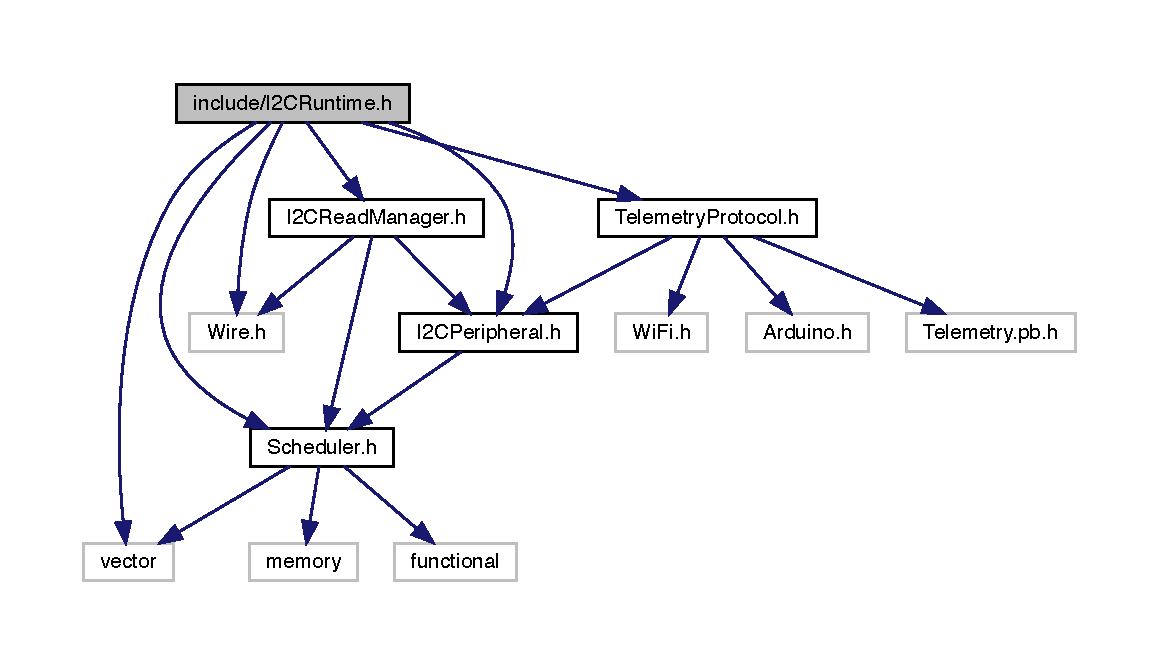
\includegraphics[width=350pt]{_i2_c_runtime_8h__incl}
\end{center}
\end{figure}
This graph shows which files directly or indirectly include this file\+:\nopagebreak
\begin{figure}[H]
\begin{center}
\leavevmode
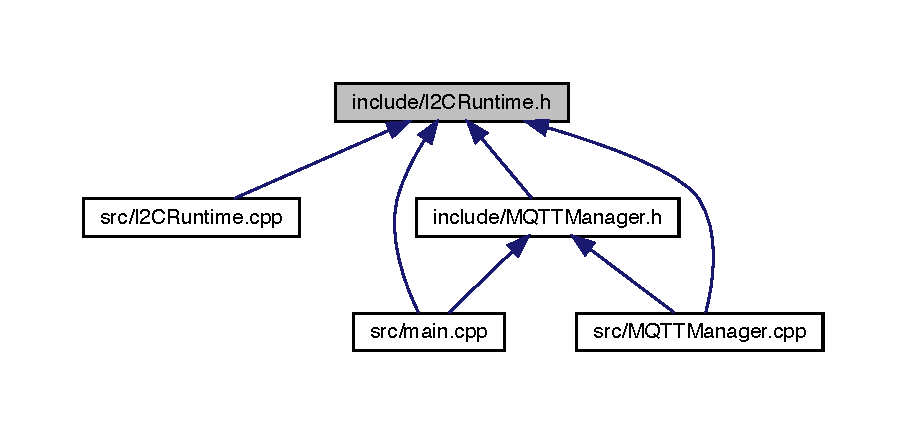
\includegraphics[width=350pt]{_i2_c_runtime_8h__dep__incl}
\end{center}
\end{figure}
\subsection*{Classes}
\begin{DoxyCompactItemize}
\item 
class \mbox{\hyperlink{class_i2_c_peripheral_manager}{I2\+C\+Peripheral\+Manager}}
\begin{DoxyCompactList}\small\item\em Manages all the read managers and memory allocation for a single peripheral. \end{DoxyCompactList}\item 
class \mbox{\hyperlink{class_i2_c_runtime}{I2\+C\+Runtime}}
\begin{DoxyCompactList}\small\item\em Responsible for the primary event loop for all peripherals on the bus. \end{DoxyCompactList}\end{DoxyCompactItemize}

\hypertarget{_m_q_t_t_manager_8h}{}\section{include/\+M\+Q\+T\+T\+Manager.h File Reference}
\label{_m_q_t_t_manager_8h}\index{include/\+M\+Q\+T\+T\+Manager.\+h@{include/\+M\+Q\+T\+T\+Manager.\+h}}
{\ttfamily \#include $<$Preferences.\+h$>$}\newline
{\ttfamily \#include $<$Pub\+Sub\+Client.\+h$>$}\newline
{\ttfamily \#include $<$Wi\+Fi.\+h$>$}\newline
{\ttfamily \#include \char`\"{}I2\+C\+Runtime.\+h\char`\"{}}\newline
{\ttfamily \#include \char`\"{}Scheduler.\+h\char`\"{}}\newline
{\ttfamily \#include \char`\"{}Telemetry\+Protocol.\+h\char`\"{}}\newline
Include dependency graph for M\+Q\+T\+T\+Manager.\+h\+:\nopagebreak
\begin{figure}[H]
\begin{center}
\leavevmode
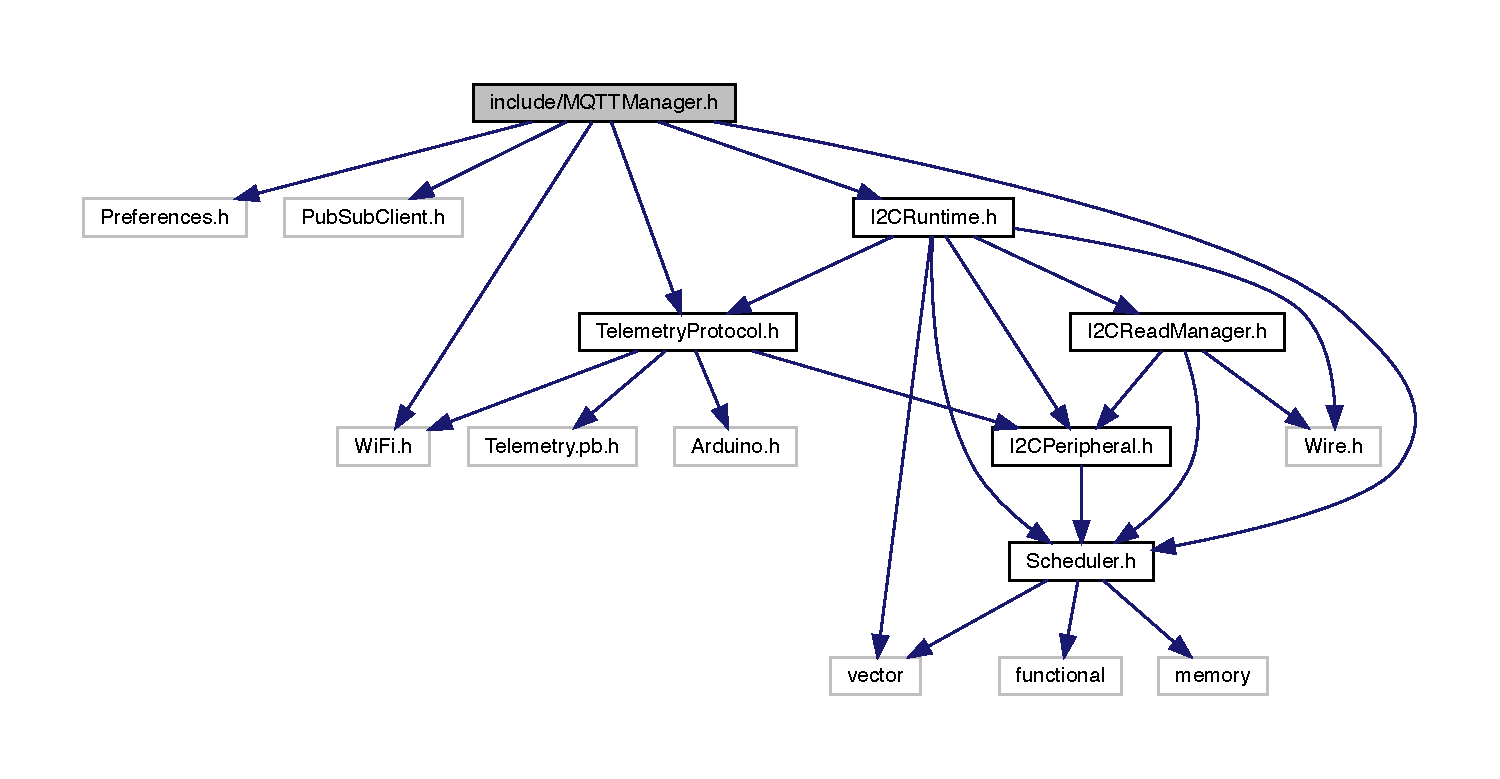
\includegraphics[width=350pt]{_m_q_t_t_manager_8h__incl}
\end{center}
\end{figure}
This graph shows which files directly or indirectly include this file\+:\nopagebreak
\begin{figure}[H]
\begin{center}
\leavevmode
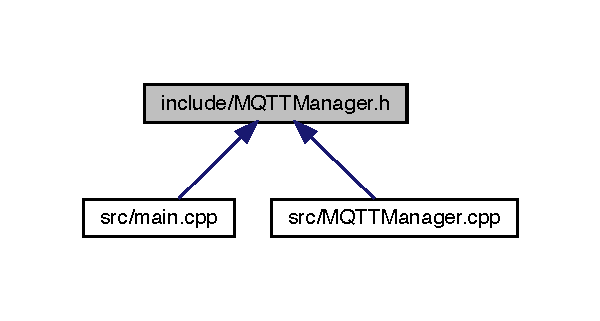
\includegraphics[width=288pt]{_m_q_t_t_manager_8h__dep__incl}
\end{center}
\end{figure}
\subsection*{Classes}
\begin{DoxyCompactItemize}
\item 
class \mbox{\hyperlink{class_m_q_t_t_manager}{M\+Q\+T\+T\+Manager}}
\begin{DoxyCompactList}\small\item\em Responsible for publishing and subscribing to topics on the M\+Q\+TT broker. \end{DoxyCompactList}\end{DoxyCompactItemize}

\hypertarget{_scheduler_8h}{}\section{include/\+Scheduler.h File Reference}
\label{_scheduler_8h}\index{include/\+Scheduler.\+h@{include/\+Scheduler.\+h}}
{\ttfamily \#include $<$functional$>$}\newline
{\ttfamily \#include $<$memory$>$}\newline
{\ttfamily \#include $<$vector$>$}\newline
Include dependency graph for Scheduler.\+h\+:\nopagebreak
\begin{figure}[H]
\begin{center}
\leavevmode
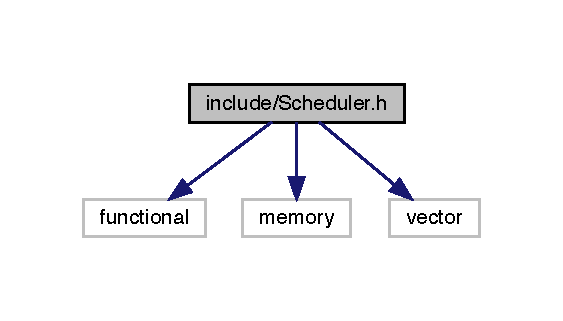
\includegraphics[width=270pt]{_scheduler_8h__incl}
\end{center}
\end{figure}
This graph shows which files directly or indirectly include this file\+:\nopagebreak
\begin{figure}[H]
\begin{center}
\leavevmode
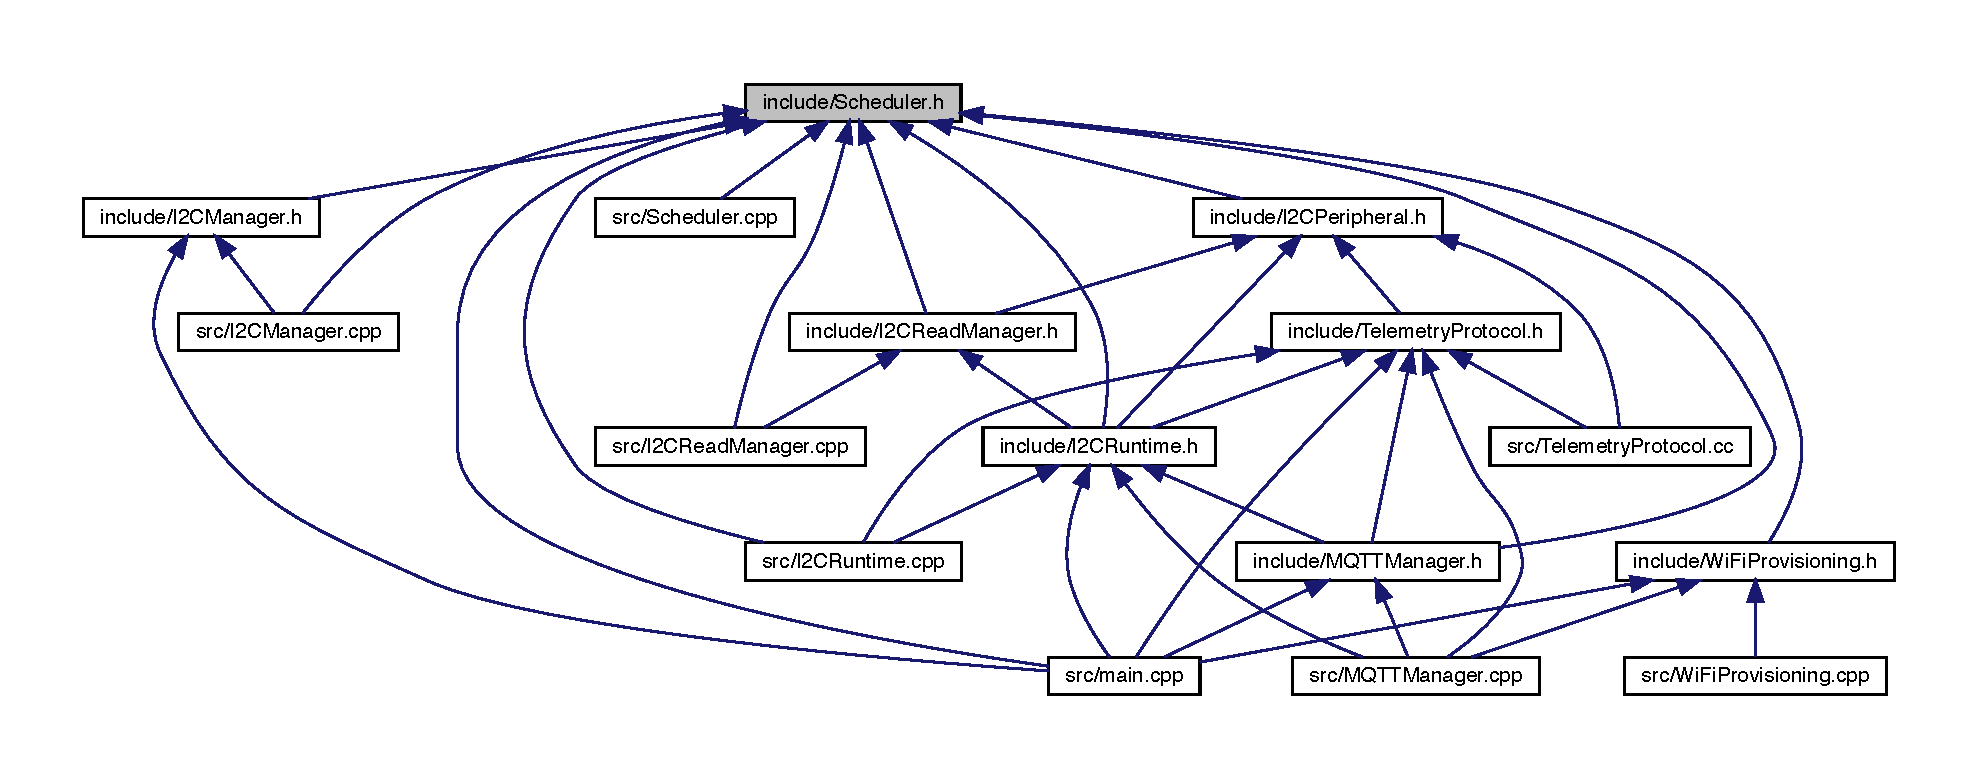
\includegraphics[width=350pt]{_scheduler_8h__dep__incl}
\end{center}
\end{figure}
\subsection*{Classes}
\begin{DoxyCompactItemize}
\item 
struct \mbox{\hyperlink{struct_schedule}{Schedule}}
\begin{DoxyCompactList}\small\item\em Declarative configuration for a managed schedule. \end{DoxyCompactList}\item 
class \mbox{\hyperlink{class_scheduler}{Scheduler}}
\begin{DoxyCompactList}\small\item\em Generic scheduler for non-\/blocking tasks given schedules for callbacks. \end{DoxyCompactList}\end{DoxyCompactItemize}
\subsection*{Macros}
\begin{DoxyCompactItemize}
\item 
\#define \mbox{\hyperlink{_scheduler_8h_a240827577ed9cf28cff316085ea5fb16}{H\+A\+S\+\_\+\+N\+E\+V\+E\+R\+\_\+\+R\+A\+N\+\_\+\+T\+I\+M\+E\+S\+T\+A\+MP}}~0
\end{DoxyCompactItemize}
\subsection*{Typedefs}
\begin{DoxyCompactItemize}
\item 
typedef uint32\+\_\+t \mbox{\hyperlink{_scheduler_8h_a7ea5c3593e888e0396e712316a491ab7}{Milli}}
\item 
typedef \mbox{\hyperlink{_scheduler_8h_a7ea5c3593e888e0396e712316a491ab7}{Milli}} \mbox{\hyperlink{_scheduler_8h_aca1fa1a7edde6bf9e22c7617400fad31}{Duration}}
\item 
typedef \mbox{\hyperlink{_scheduler_8h_a7ea5c3593e888e0396e712316a491ab7}{Milli}} \mbox{\hyperlink{_scheduler_8h_a67c6ac2398ae81344762ebb1b71fc9a7}{Timestamp}}
\item 
typedef std\+::function$<$ void()$>$ \mbox{\hyperlink{_scheduler_8h_a2125a5a2949d6ee13163b671159c0d4d}{Func}}
\item 
typedef std\+::size\+\_\+t \mbox{\hyperlink{_scheduler_8h_a1e3b4605bdcbb8f6df7c47013e26e910}{Schedule\+Id}}
\end{DoxyCompactItemize}


\subsection{Macro Definition Documentation}
\mbox{\Hypertarget{_scheduler_8h_a240827577ed9cf28cff316085ea5fb16}\label{_scheduler_8h_a240827577ed9cf28cff316085ea5fb16}} 
\index{Scheduler.\+h@{Scheduler.\+h}!H\+A\+S\+\_\+\+N\+E\+V\+E\+R\+\_\+\+R\+A\+N\+\_\+\+T\+I\+M\+E\+S\+T\+A\+MP@{H\+A\+S\+\_\+\+N\+E\+V\+E\+R\+\_\+\+R\+A\+N\+\_\+\+T\+I\+M\+E\+S\+T\+A\+MP}}
\index{H\+A\+S\+\_\+\+N\+E\+V\+E\+R\+\_\+\+R\+A\+N\+\_\+\+T\+I\+M\+E\+S\+T\+A\+MP@{H\+A\+S\+\_\+\+N\+E\+V\+E\+R\+\_\+\+R\+A\+N\+\_\+\+T\+I\+M\+E\+S\+T\+A\+MP}!Scheduler.\+h@{Scheduler.\+h}}
\subsubsection{\texorpdfstring{H\+A\+S\+\_\+\+N\+E\+V\+E\+R\+\_\+\+R\+A\+N\+\_\+\+T\+I\+M\+E\+S\+T\+A\+MP}{HAS\_NEVER\_RAN\_TIMESTAMP}}
{\footnotesize\ttfamily \#define H\+A\+S\+\_\+\+N\+E\+V\+E\+R\+\_\+\+R\+A\+N\+\_\+\+T\+I\+M\+E\+S\+T\+A\+MP~0}



\subsection{Typedef Documentation}
\mbox{\Hypertarget{_scheduler_8h_aca1fa1a7edde6bf9e22c7617400fad31}\label{_scheduler_8h_aca1fa1a7edde6bf9e22c7617400fad31}} 
\index{Scheduler.\+h@{Scheduler.\+h}!Duration@{Duration}}
\index{Duration@{Duration}!Scheduler.\+h@{Scheduler.\+h}}
\subsubsection{\texorpdfstring{Duration}{Duration}}
{\footnotesize\ttfamily typedef \mbox{\hyperlink{_scheduler_8h_a7ea5c3593e888e0396e712316a491ab7}{Milli}} \mbox{\hyperlink{_scheduler_8h_aca1fa1a7edde6bf9e22c7617400fad31}{Duration}}}

\mbox{\Hypertarget{_scheduler_8h_a2125a5a2949d6ee13163b671159c0d4d}\label{_scheduler_8h_a2125a5a2949d6ee13163b671159c0d4d}} 
\index{Scheduler.\+h@{Scheduler.\+h}!Func@{Func}}
\index{Func@{Func}!Scheduler.\+h@{Scheduler.\+h}}
\subsubsection{\texorpdfstring{Func}{Func}}
{\footnotesize\ttfamily typedef std\+::function$<$void ()$>$ \mbox{\hyperlink{_scheduler_8h_a2125a5a2949d6ee13163b671159c0d4d}{Func}}}

\mbox{\Hypertarget{_scheduler_8h_a7ea5c3593e888e0396e712316a491ab7}\label{_scheduler_8h_a7ea5c3593e888e0396e712316a491ab7}} 
\index{Scheduler.\+h@{Scheduler.\+h}!Milli@{Milli}}
\index{Milli@{Milli}!Scheduler.\+h@{Scheduler.\+h}}
\subsubsection{\texorpdfstring{Milli}{Milli}}
{\footnotesize\ttfamily typedef uint32\+\_\+t \mbox{\hyperlink{_scheduler_8h_a7ea5c3593e888e0396e712316a491ab7}{Milli}}}

\mbox{\Hypertarget{_scheduler_8h_a1e3b4605bdcbb8f6df7c47013e26e910}\label{_scheduler_8h_a1e3b4605bdcbb8f6df7c47013e26e910}} 
\index{Scheduler.\+h@{Scheduler.\+h}!Schedule\+Id@{Schedule\+Id}}
\index{Schedule\+Id@{Schedule\+Id}!Scheduler.\+h@{Scheduler.\+h}}
\subsubsection{\texorpdfstring{Schedule\+Id}{ScheduleId}}
{\footnotesize\ttfamily typedef std\+::size\+\_\+t \mbox{\hyperlink{_scheduler_8h_a1e3b4605bdcbb8f6df7c47013e26e910}{Schedule\+Id}}}

\mbox{\Hypertarget{_scheduler_8h_a67c6ac2398ae81344762ebb1b71fc9a7}\label{_scheduler_8h_a67c6ac2398ae81344762ebb1b71fc9a7}} 
\index{Scheduler.\+h@{Scheduler.\+h}!Timestamp@{Timestamp}}
\index{Timestamp@{Timestamp}!Scheduler.\+h@{Scheduler.\+h}}
\subsubsection{\texorpdfstring{Timestamp}{Timestamp}}
{\footnotesize\ttfamily typedef \mbox{\hyperlink{_scheduler_8h_a7ea5c3593e888e0396e712316a491ab7}{Milli}} \mbox{\hyperlink{_scheduler_8h_a67c6ac2398ae81344762ebb1b71fc9a7}{Timestamp}}}


\hypertarget{_telemetry_protocol_8h}{}\section{include/\+Telemetry\+Protocol.h File Reference}
\label{_telemetry_protocol_8h}\index{include/\+Telemetry\+Protocol.\+h@{include/\+Telemetry\+Protocol.\+h}}
{\ttfamily \#include $<$Arduino.\+h$>$}\newline
{\ttfamily \#include $<$Telemetry.\+pb.\+h$>$}\newline
{\ttfamily \#include $<$Wi\+Fi.\+h$>$}\newline
{\ttfamily \#include \char`\"{}I2\+C\+Peripheral.\+h\char`\"{}}\newline
Include dependency graph for Telemetry\+Protocol.\+h\+:\nopagebreak
\begin{figure}[H]
\begin{center}
\leavevmode
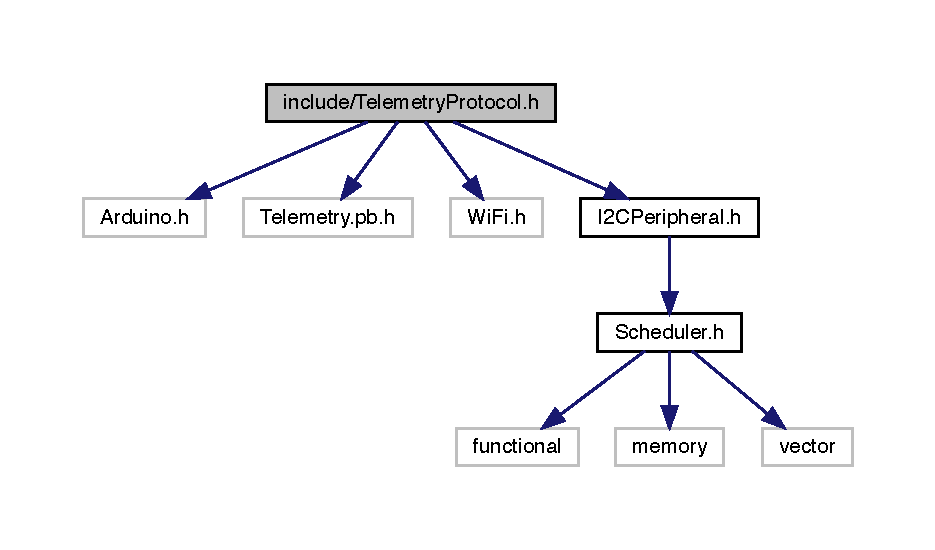
\includegraphics[width=350pt]{_telemetry_protocol_8h__incl}
\end{center}
\end{figure}
This graph shows which files directly or indirectly include this file\+:\nopagebreak
\begin{figure}[H]
\begin{center}
\leavevmode
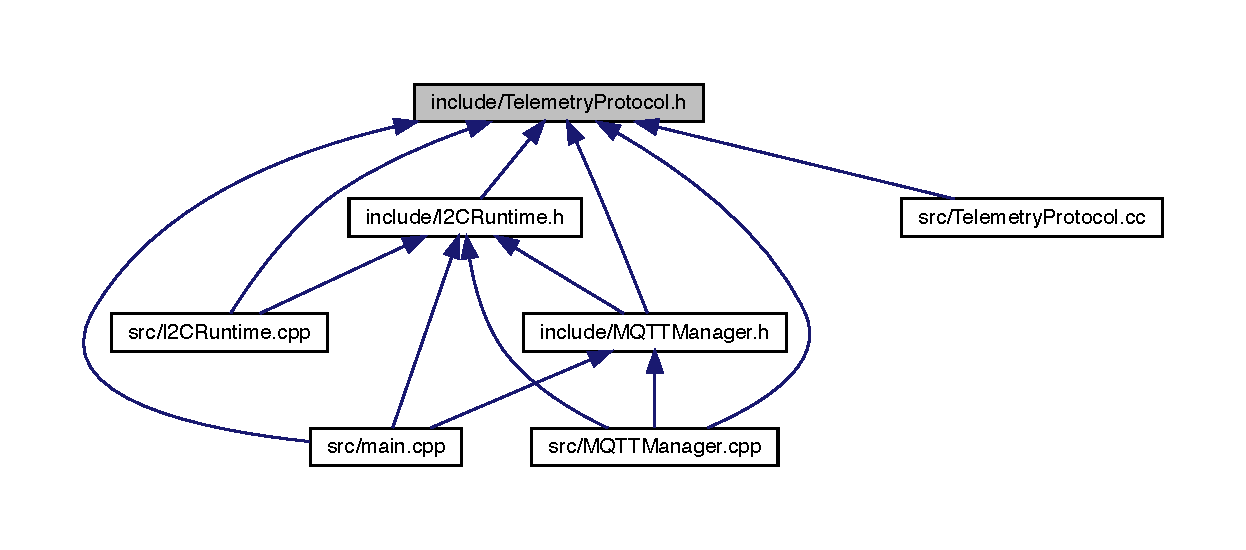
\includegraphics[width=350pt]{_telemetry_protocol_8h__dep__incl}
\end{center}
\end{figure}
\subsection*{Classes}
\begin{DoxyCompactItemize}
\item 
struct \mbox{\hyperlink{struct_peripheral_status}{Peripheral\+Status}}
\begin{DoxyCompactList}\small\item\em Intermediate object for protobuf encoding. \end{DoxyCompactList}\item 
class \mbox{\hyperlink{class_telemetry_protocol}{Telemetry\+Protocol}}
\begin{DoxyCompactList}\small\item\em Responsible for encoding and decoding protobuf/nanopb payloads. \end{DoxyCompactList}\end{DoxyCompactItemize}
\subsection*{Typedefs}
\begin{DoxyCompactItemize}
\item 
typedef std\+::function$<$ void(uint32\+\_\+t, uint16\+\_\+t, \mbox{\hyperlink{struct_read_definition}{Read\+Definition}} $\ast$, uint8\+\_\+t $\ast$)$>$ \mbox{\hyperlink{_telemetry_protocol_8h_a98c05796bd59110e8ae10dc71580b759}{Payload\+Func}}
\item 
typedef struct \mbox{\hyperlink{struct_peripheral_status}{Peripheral\+Status}} \mbox{\hyperlink{_telemetry_protocol_8h_a2b53b967d745b3b918f0d6f97305d109}{Peripheral\+Status}}
\end{DoxyCompactItemize}


\subsection{Typedef Documentation}
\mbox{\Hypertarget{_telemetry_protocol_8h_a98c05796bd59110e8ae10dc71580b759}\label{_telemetry_protocol_8h_a98c05796bd59110e8ae10dc71580b759}} 
\index{Telemetry\+Protocol.\+h@{Telemetry\+Protocol.\+h}!Payload\+Func@{Payload\+Func}}
\index{Payload\+Func@{Payload\+Func}!Telemetry\+Protocol.\+h@{Telemetry\+Protocol.\+h}}
\subsubsection{\texorpdfstring{Payload\+Func}{PayloadFunc}}
{\footnotesize\ttfamily typedef std\+::function$<$void (uint32\+\_\+t, uint16\+\_\+t, \mbox{\hyperlink{struct_read_definition}{Read\+Definition}} $\ast$, uint8\+\_\+t $\ast$)$>$ \mbox{\hyperlink{_telemetry_protocol_8h_a98c05796bd59110e8ae10dc71580b759}{Payload\+Func}}}

\mbox{\Hypertarget{_telemetry_protocol_8h_a2b53b967d745b3b918f0d6f97305d109}\label{_telemetry_protocol_8h_a2b53b967d745b3b918f0d6f97305d109}} 
\index{Telemetry\+Protocol.\+h@{Telemetry\+Protocol.\+h}!Peripheral\+Status@{Peripheral\+Status}}
\index{Peripheral\+Status@{Peripheral\+Status}!Telemetry\+Protocol.\+h@{Telemetry\+Protocol.\+h}}
\subsubsection{\texorpdfstring{Peripheral\+Status}{PeripheralStatus}}
{\footnotesize\ttfamily typedef struct \mbox{\hyperlink{struct_peripheral_status}{Peripheral\+Status}} \mbox{\hyperlink{struct_peripheral_status}{Peripheral\+Status}}}


\hypertarget{_wi_fi_provisioning_8h}{}\section{include/\+Wi\+Fi\+Provisioning.h File Reference}
\label{_wi_fi_provisioning_8h}\index{include/\+Wi\+Fi\+Provisioning.\+h@{include/\+Wi\+Fi\+Provisioning.\+h}}
{\ttfamily \#include $<$Preferences.\+h$>$}\newline
{\ttfamily \#include $<$Wi\+Fi.\+h$>$}\newline
{\ttfamily \#include $<$string$>$}\newline
{\ttfamily \#include \char`\"{}Scheduler.\+h\char`\"{}}\newline
Include dependency graph for Wi\+Fi\+Provisioning.\+h\+:\nopagebreak
\begin{figure}[H]
\begin{center}
\leavevmode
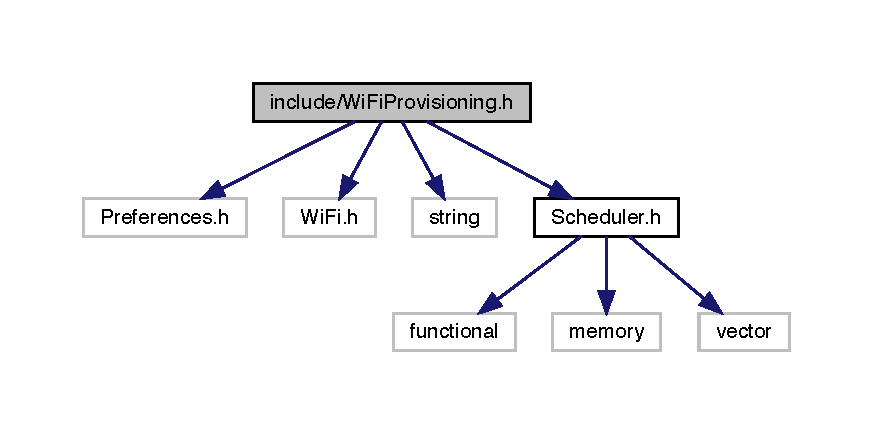
\includegraphics[width=350pt]{_wi_fi_provisioning_8h__incl}
\end{center}
\end{figure}
This graph shows which files directly or indirectly include this file\+:\nopagebreak
\begin{figure}[H]
\begin{center}
\leavevmode
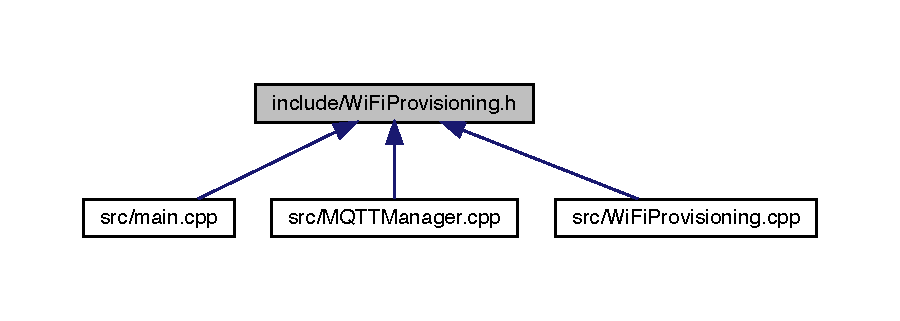
\includegraphics[width=350pt]{_wi_fi_provisioning_8h__dep__incl}
\end{center}
\end{figure}
\subsection*{Classes}
\begin{DoxyCompactItemize}
\item 
class \mbox{\hyperlink{class_wi_fi_provisioning}{Wi\+Fi\+Provisioning}}
\begin{DoxyCompactList}\small\item\em Manages the web application for provisioning connectivity information. \end{DoxyCompactList}\end{DoxyCompactItemize}
\subsection*{Macros}
\begin{DoxyCompactItemize}
\item 
\#define \mbox{\hyperlink{_wi_fi_provisioning_8h_ad8e4942e5de32671cb1eb40828699fc7}{P\+R\+O\+V\+I\+S\+I\+O\+N\+I\+N\+G\+\_\+\+A\+P\+\_\+\+S\+S\+ID}}~\char`\"{}Telemetry\+Microcontroller\char`\"{}
\item 
\#define \mbox{\hyperlink{_wi_fi_provisioning_8h_a936c8fcf7641cc49c7f39eed91c76f49}{P\+R\+O\+V\+I\+S\+I\+O\+N\+I\+N\+G\+\_\+\+A\+P\+\_\+\+P\+A\+SS}}~\char`\"{}4zp6capstone\char`\"{}
\item 
\#define \mbox{\hyperlink{_wi_fi_provisioning_8h_ada1f8cf66be69bbc0a45fd6b12206ffe}{P\+R\+O\+V\+I\+S\+I\+O\+N\+I\+N\+G\+\_\+\+C\+O\+N\+N\+E\+C\+T\+I\+O\+N\+\_\+\+A\+T\+T\+E\+M\+P\+T\+\_\+\+L\+I\+M\+IT}}~10
\item 
\#define \mbox{\hyperlink{_wi_fi_provisioning_8h_a8ffe66aa5051ca397a18eb7c63e96962}{P\+R\+E\+F\+E\+R\+E\+N\+C\+E\+S\+\_\+\+N\+A\+M\+E\+S\+P\+A\+CE}}~\char`\"{}telemetry\char`\"{}
\item 
\#define \mbox{\hyperlink{_wi_fi_provisioning_8h_a16c2786c70e077c5af785472d73bdb65}{W\+E\+B\+\_\+\+S\+E\+R\+V\+E\+R\+\_\+\+T\+I\+M\+E\+O\+UT}}~1000
\end{DoxyCompactItemize}
\subsection*{Functions}
\begin{DoxyCompactItemize}
\item 
void \mbox{\hyperlink{_wi_fi_provisioning_8h_a15be4380984c85a00d34729245710d4c}{replace}} (std\+::string \&haystack, std\+::string needle, const char $\ast$replacement)
\end{DoxyCompactItemize}


\subsection{Macro Definition Documentation}
\mbox{\Hypertarget{_wi_fi_provisioning_8h_a8ffe66aa5051ca397a18eb7c63e96962}\label{_wi_fi_provisioning_8h_a8ffe66aa5051ca397a18eb7c63e96962}} 
\index{Wi\+Fi\+Provisioning.\+h@{Wi\+Fi\+Provisioning.\+h}!P\+R\+E\+F\+E\+R\+E\+N\+C\+E\+S\+\_\+\+N\+A\+M\+E\+S\+P\+A\+CE@{P\+R\+E\+F\+E\+R\+E\+N\+C\+E\+S\+\_\+\+N\+A\+M\+E\+S\+P\+A\+CE}}
\index{P\+R\+E\+F\+E\+R\+E\+N\+C\+E\+S\+\_\+\+N\+A\+M\+E\+S\+P\+A\+CE@{P\+R\+E\+F\+E\+R\+E\+N\+C\+E\+S\+\_\+\+N\+A\+M\+E\+S\+P\+A\+CE}!Wi\+Fi\+Provisioning.\+h@{Wi\+Fi\+Provisioning.\+h}}
\subsubsection{\texorpdfstring{P\+R\+E\+F\+E\+R\+E\+N\+C\+E\+S\+\_\+\+N\+A\+M\+E\+S\+P\+A\+CE}{PREFERENCES\_NAMESPACE}}
{\footnotesize\ttfamily \#define P\+R\+E\+F\+E\+R\+E\+N\+C\+E\+S\+\_\+\+N\+A\+M\+E\+S\+P\+A\+CE~\char`\"{}telemetry\char`\"{}}

\mbox{\Hypertarget{_wi_fi_provisioning_8h_a936c8fcf7641cc49c7f39eed91c76f49}\label{_wi_fi_provisioning_8h_a936c8fcf7641cc49c7f39eed91c76f49}} 
\index{Wi\+Fi\+Provisioning.\+h@{Wi\+Fi\+Provisioning.\+h}!P\+R\+O\+V\+I\+S\+I\+O\+N\+I\+N\+G\+\_\+\+A\+P\+\_\+\+P\+A\+SS@{P\+R\+O\+V\+I\+S\+I\+O\+N\+I\+N\+G\+\_\+\+A\+P\+\_\+\+P\+A\+SS}}
\index{P\+R\+O\+V\+I\+S\+I\+O\+N\+I\+N\+G\+\_\+\+A\+P\+\_\+\+P\+A\+SS@{P\+R\+O\+V\+I\+S\+I\+O\+N\+I\+N\+G\+\_\+\+A\+P\+\_\+\+P\+A\+SS}!Wi\+Fi\+Provisioning.\+h@{Wi\+Fi\+Provisioning.\+h}}
\subsubsection{\texorpdfstring{P\+R\+O\+V\+I\+S\+I\+O\+N\+I\+N\+G\+\_\+\+A\+P\+\_\+\+P\+A\+SS}{PROVISIONING\_AP\_PASS}}
{\footnotesize\ttfamily \#define P\+R\+O\+V\+I\+S\+I\+O\+N\+I\+N\+G\+\_\+\+A\+P\+\_\+\+P\+A\+SS~\char`\"{}4zp6capstone\char`\"{}}

\mbox{\Hypertarget{_wi_fi_provisioning_8h_ad8e4942e5de32671cb1eb40828699fc7}\label{_wi_fi_provisioning_8h_ad8e4942e5de32671cb1eb40828699fc7}} 
\index{Wi\+Fi\+Provisioning.\+h@{Wi\+Fi\+Provisioning.\+h}!P\+R\+O\+V\+I\+S\+I\+O\+N\+I\+N\+G\+\_\+\+A\+P\+\_\+\+S\+S\+ID@{P\+R\+O\+V\+I\+S\+I\+O\+N\+I\+N\+G\+\_\+\+A\+P\+\_\+\+S\+S\+ID}}
\index{P\+R\+O\+V\+I\+S\+I\+O\+N\+I\+N\+G\+\_\+\+A\+P\+\_\+\+S\+S\+ID@{P\+R\+O\+V\+I\+S\+I\+O\+N\+I\+N\+G\+\_\+\+A\+P\+\_\+\+S\+S\+ID}!Wi\+Fi\+Provisioning.\+h@{Wi\+Fi\+Provisioning.\+h}}
\subsubsection{\texorpdfstring{P\+R\+O\+V\+I\+S\+I\+O\+N\+I\+N\+G\+\_\+\+A\+P\+\_\+\+S\+S\+ID}{PROVISIONING\_AP\_SSID}}
{\footnotesize\ttfamily \#define P\+R\+O\+V\+I\+S\+I\+O\+N\+I\+N\+G\+\_\+\+A\+P\+\_\+\+S\+S\+ID~\char`\"{}Telemetry\+Microcontroller\char`\"{}}

\mbox{\Hypertarget{_wi_fi_provisioning_8h_ada1f8cf66be69bbc0a45fd6b12206ffe}\label{_wi_fi_provisioning_8h_ada1f8cf66be69bbc0a45fd6b12206ffe}} 
\index{Wi\+Fi\+Provisioning.\+h@{Wi\+Fi\+Provisioning.\+h}!P\+R\+O\+V\+I\+S\+I\+O\+N\+I\+N\+G\+\_\+\+C\+O\+N\+N\+E\+C\+T\+I\+O\+N\+\_\+\+A\+T\+T\+E\+M\+P\+T\+\_\+\+L\+I\+M\+IT@{P\+R\+O\+V\+I\+S\+I\+O\+N\+I\+N\+G\+\_\+\+C\+O\+N\+N\+E\+C\+T\+I\+O\+N\+\_\+\+A\+T\+T\+E\+M\+P\+T\+\_\+\+L\+I\+M\+IT}}
\index{P\+R\+O\+V\+I\+S\+I\+O\+N\+I\+N\+G\+\_\+\+C\+O\+N\+N\+E\+C\+T\+I\+O\+N\+\_\+\+A\+T\+T\+E\+M\+P\+T\+\_\+\+L\+I\+M\+IT@{P\+R\+O\+V\+I\+S\+I\+O\+N\+I\+N\+G\+\_\+\+C\+O\+N\+N\+E\+C\+T\+I\+O\+N\+\_\+\+A\+T\+T\+E\+M\+P\+T\+\_\+\+L\+I\+M\+IT}!Wi\+Fi\+Provisioning.\+h@{Wi\+Fi\+Provisioning.\+h}}
\subsubsection{\texorpdfstring{P\+R\+O\+V\+I\+S\+I\+O\+N\+I\+N\+G\+\_\+\+C\+O\+N\+N\+E\+C\+T\+I\+O\+N\+\_\+\+A\+T\+T\+E\+M\+P\+T\+\_\+\+L\+I\+M\+IT}{PROVISIONING\_CONNECTION\_ATTEMPT\_LIMIT}}
{\footnotesize\ttfamily \#define P\+R\+O\+V\+I\+S\+I\+O\+N\+I\+N\+G\+\_\+\+C\+O\+N\+N\+E\+C\+T\+I\+O\+N\+\_\+\+A\+T\+T\+E\+M\+P\+T\+\_\+\+L\+I\+M\+IT~10}

\mbox{\Hypertarget{_wi_fi_provisioning_8h_a16c2786c70e077c5af785472d73bdb65}\label{_wi_fi_provisioning_8h_a16c2786c70e077c5af785472d73bdb65}} 
\index{Wi\+Fi\+Provisioning.\+h@{Wi\+Fi\+Provisioning.\+h}!W\+E\+B\+\_\+\+S\+E\+R\+V\+E\+R\+\_\+\+T\+I\+M\+E\+O\+UT@{W\+E\+B\+\_\+\+S\+E\+R\+V\+E\+R\+\_\+\+T\+I\+M\+E\+O\+UT}}
\index{W\+E\+B\+\_\+\+S\+E\+R\+V\+E\+R\+\_\+\+T\+I\+M\+E\+O\+UT@{W\+E\+B\+\_\+\+S\+E\+R\+V\+E\+R\+\_\+\+T\+I\+M\+E\+O\+UT}!Wi\+Fi\+Provisioning.\+h@{Wi\+Fi\+Provisioning.\+h}}
\subsubsection{\texorpdfstring{W\+E\+B\+\_\+\+S\+E\+R\+V\+E\+R\+\_\+\+T\+I\+M\+E\+O\+UT}{WEB\_SERVER\_TIMEOUT}}
{\footnotesize\ttfamily \#define W\+E\+B\+\_\+\+S\+E\+R\+V\+E\+R\+\_\+\+T\+I\+M\+E\+O\+UT~1000}



\subsection{Function Documentation}
\mbox{\Hypertarget{_wi_fi_provisioning_8h_a15be4380984c85a00d34729245710d4c}\label{_wi_fi_provisioning_8h_a15be4380984c85a00d34729245710d4c}} 
\index{Wi\+Fi\+Provisioning.\+h@{Wi\+Fi\+Provisioning.\+h}!replace@{replace}}
\index{replace@{replace}!Wi\+Fi\+Provisioning.\+h@{Wi\+Fi\+Provisioning.\+h}}
\subsubsection{\texorpdfstring{replace()}{replace()}}
{\footnotesize\ttfamily void replace (\begin{DoxyParamCaption}\item[{std\+::string \&}]{haystack,  }\item[{std\+::string}]{needle,  }\item[{const char $\ast$}]{replacement }\end{DoxyParamCaption})}


\hypertarget{_i2_c_manager_8cpp}{}\section{src/\+I2\+C\+Manager.cpp File Reference}
\label{_i2_c_manager_8cpp}\index{src/\+I2\+C\+Manager.\+cpp@{src/\+I2\+C\+Manager.\+cpp}}
{\ttfamily \#include $<$Arduino.\+h$>$}\newline
{\ttfamily \#include $<$functional$>$}\newline
{\ttfamily \#include $<$memory$>$}\newline
{\ttfamily \#include \char`\"{}I2\+C\+Manager.\+h\char`\"{}}\newline
{\ttfamily \#include \char`\"{}Scheduler.\+h\char`\"{}}\newline
Include dependency graph for I2\+C\+Manager.\+cpp\+:\nopagebreak
\begin{figure}[H]
\begin{center}
\leavevmode
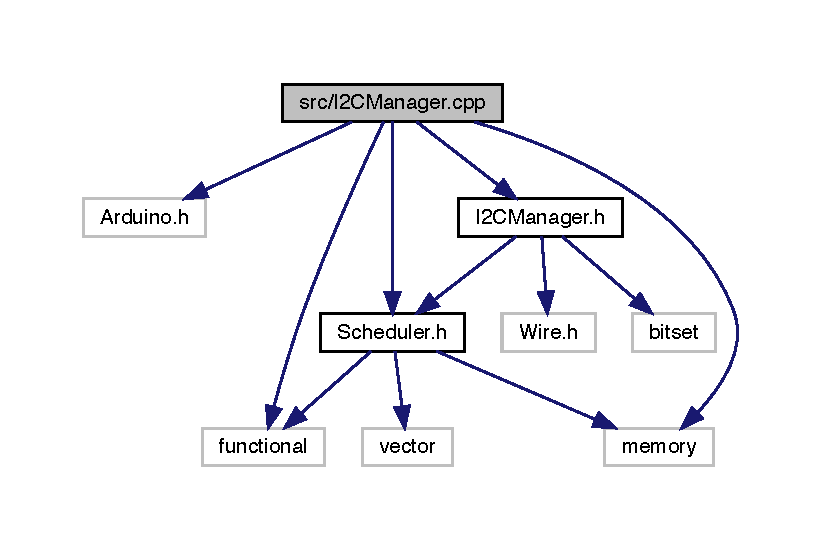
\includegraphics[width=350pt]{_i2_c_manager_8cpp__incl}
\end{center}
\end{figure}

\hypertarget{_i2_c_read_manager_8cpp}{}\section{src/\+I2\+C\+Read\+Manager.cpp File Reference}
\label{_i2_c_read_manager_8cpp}\index{src/\+I2\+C\+Read\+Manager.\+cpp@{src/\+I2\+C\+Read\+Manager.\+cpp}}
{\ttfamily \#include $<$Arduino.\+h$>$}\newline
{\ttfamily \#include $<$Wire.\+h$>$}\newline
{\ttfamily \#include \char`\"{}I2\+C\+Read\+Manager.\+h\char`\"{}}\newline
{\ttfamily \#include \char`\"{}Scheduler.\+h\char`\"{}}\newline
Include dependency graph for I2\+C\+Read\+Manager.\+cpp\+:\nopagebreak
\begin{figure}[H]
\begin{center}
\leavevmode
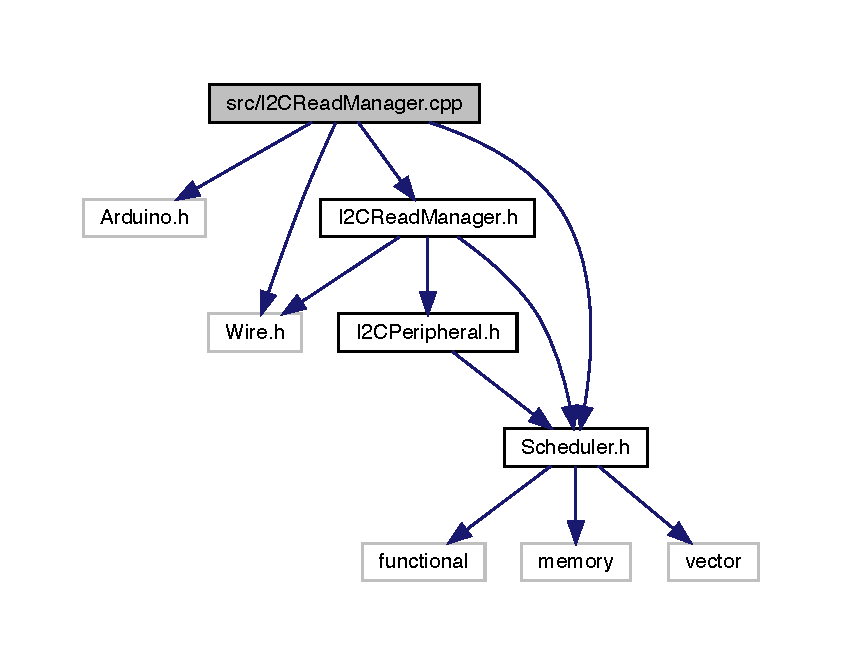
\includegraphics[width=350pt]{_i2_c_read_manager_8cpp__incl}
\end{center}
\end{figure}

\hypertarget{_i2_c_runtime_8cpp}{}\section{src/\+I2\+C\+Runtime.cpp File Reference}
\label{_i2_c_runtime_8cpp}\index{src/\+I2\+C\+Runtime.\+cpp@{src/\+I2\+C\+Runtime.\+cpp}}
{\ttfamily \#include $<$Arduino.\+h$>$}\newline
{\ttfamily \#include $<$vector$>$}\newline
{\ttfamily \#include $<$Wire.\+h$>$}\newline
{\ttfamily \#include \char`\"{}I2\+C\+Runtime.\+h\char`\"{}}\newline
{\ttfamily \#include \char`\"{}Scheduler.\+h\char`\"{}}\newline
{\ttfamily \#include \char`\"{}Telemetry\+Protocol.\+h\char`\"{}}\newline
Include dependency graph for I2\+C\+Runtime.\+cpp\+:\nopagebreak
\begin{figure}[H]
\begin{center}
\leavevmode
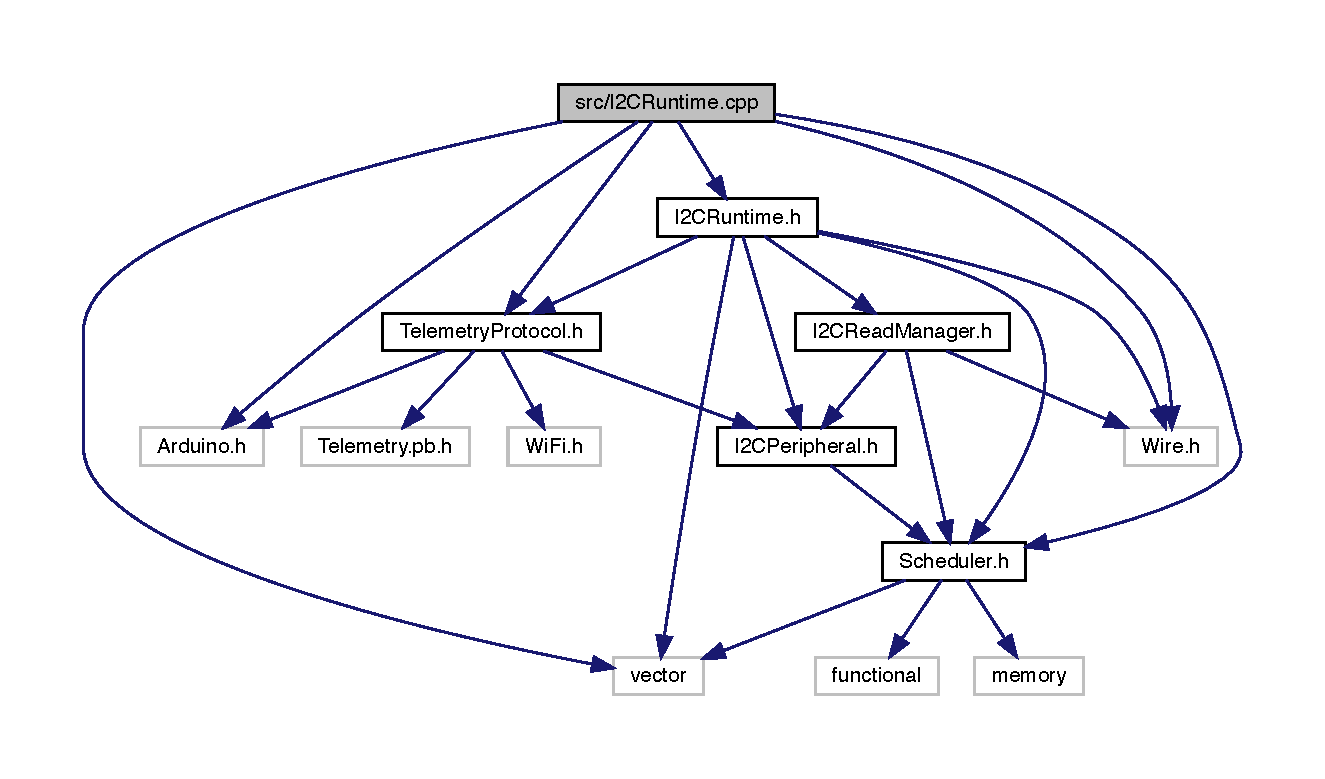
\includegraphics[width=350pt]{_i2_c_runtime_8cpp__incl}
\end{center}
\end{figure}

\hypertarget{main_8cpp}{}\section{src/main.cpp File Reference}
\label{main_8cpp}\index{src/main.\+cpp@{src/main.\+cpp}}
{\ttfamily \#include $<$Arduino.\+h$>$}\newline
{\ttfamily \#include $<$functional$>$}\newline
{\ttfamily \#include $<$memory$>$}\newline
{\ttfamily \#include $<$Wi\+Fi.\+h$>$}\newline
{\ttfamily \#include $<$Wire.\+h$>$}\newline
{\ttfamily \#include \char`\"{}I2\+C\+Manager.\+h\char`\"{}}\newline
{\ttfamily \#include \char`\"{}I2\+C\+Runtime.\+h\char`\"{}}\newline
{\ttfamily \#include \char`\"{}M\+Q\+T\+T\+Manager.\+h\char`\"{}}\newline
{\ttfamily \#include \char`\"{}Scheduler.\+h\char`\"{}}\newline
{\ttfamily \#include \char`\"{}Wi\+Fi\+Provisioning.\+h\char`\"{}}\newline
{\ttfamily \#include \char`\"{}Telemetry\+Protocol.\+h\char`\"{}}\newline
Include dependency graph for main.\+cpp\+:\nopagebreak
\begin{figure}[H]
\begin{center}
\leavevmode
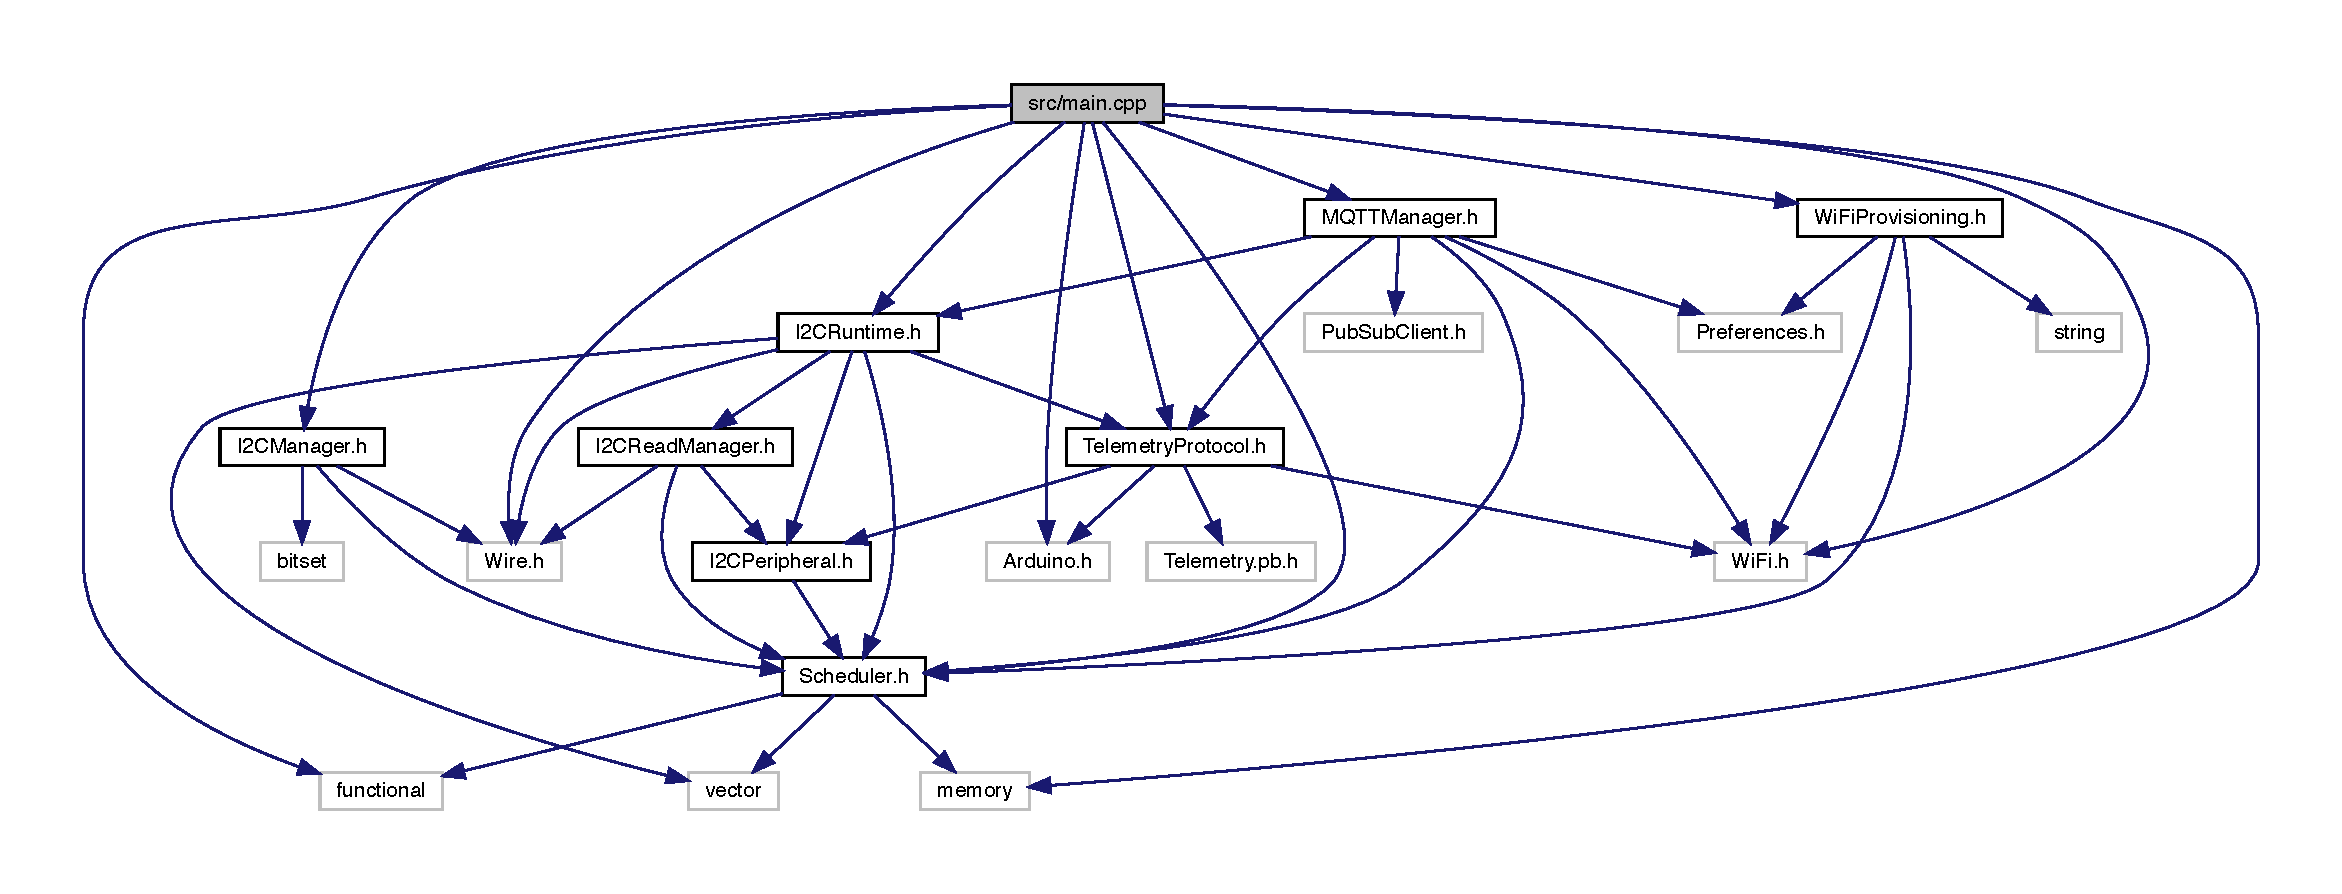
\includegraphics[width=350pt]{main_8cpp__incl}
\end{center}
\end{figure}
\subsection*{Macros}
\begin{DoxyCompactItemize}
\item 
\#define \mbox{\hyperlink{main_8cpp_aa68f159f20de602f702ea3d20b170d48}{E\+N\+A\+B\+L\+E\+\_\+\+P\+R\+O\+V\+I\+S\+I\+O\+N\+I\+NG}}
\item 
\#define \mbox{\hyperlink{main_8cpp_adcb54b1cb18cbbd88740c59e0d218dd3}{E\+N\+A\+B\+L\+E\+\_\+\+P\+E\+R\+I\+P\+H\+E\+R\+A\+LS}}
\item 
\#define \mbox{\hyperlink{main_8cpp_a29f56c86e44d58984056615782d3908c}{E\+N\+A\+B\+L\+E\+\_\+\+M\+Q\+TT}}
\end{DoxyCompactItemize}
\subsection*{Functions}
\begin{DoxyCompactItemize}
\item 
void \mbox{\hyperlink{main_8cpp_a4fc01d736fe50cf5b977f755b675f11d}{setup}} ()
\item 
void \mbox{\hyperlink{main_8cpp_afe461d27b9c48d5921c00d521181f12f}{loop}} ()
\end{DoxyCompactItemize}
\subsection*{Variables}
\begin{DoxyCompactItemize}
\item 
Two\+Wire $\ast$ \mbox{\hyperlink{main_8cpp_ab8d8f9af97a698a5a73132c347acbaf4}{wire}} = \&Wire
\item 
\mbox{\hyperlink{class_scheduler}{Scheduler}} \mbox{\hyperlink{main_8cpp_a7714de4b56e9edd12c75f4781688edef}{scheduler}}
\item 
\mbox{\hyperlink{class_i2_c_runtime}{I2\+C\+Runtime}} \mbox{\hyperlink{main_8cpp_a1fa047c23d7c85d1ad97022cd6b157d0}{runtime}} (\mbox{\hyperlink{main_8cpp_ab8d8f9af97a698a5a73132c347acbaf4}{wire}})
\item 
\mbox{\hyperlink{class_i2_c_manager}{I2\+C\+Manager}} \mbox{\hyperlink{main_8cpp_a4bd7b89b7f58f26e84f7492132fa0300}{manager}} (\mbox{\hyperlink{main_8cpp_ab8d8f9af97a698a5a73132c347acbaf4}{wire}})
\item 
uint8\+\_\+t $\ast$$\ast$ \mbox{\hyperlink{main_8cpp_acbfc37f5d7a96b409173aafea19b3835}{sht\+Buffer}} = N\+U\+LL
\item 
\mbox{\hyperlink{class_wi_fi_provisioning}{Wi\+Fi\+Provisioning}} \mbox{\hyperlink{main_8cpp_a95595a8a87900e88776af9025f5707de}{provisioning}}
\item 
\mbox{\hyperlink{class_m_q_t_t_manager}{M\+Q\+T\+T\+Manager}} \mbox{\hyperlink{main_8cpp_ac0d9ae636df973dc6a130e24b87cb19c}{mqtt\+Manager}} (\mbox{\hyperlink{main_8cpp_a1fa047c23d7c85d1ad97022cd6b157d0}{runtime}})
\end{DoxyCompactItemize}


\subsection{Macro Definition Documentation}
\mbox{\Hypertarget{main_8cpp_a29f56c86e44d58984056615782d3908c}\label{main_8cpp_a29f56c86e44d58984056615782d3908c}} 
\index{main.\+cpp@{main.\+cpp}!E\+N\+A\+B\+L\+E\+\_\+\+M\+Q\+TT@{E\+N\+A\+B\+L\+E\+\_\+\+M\+Q\+TT}}
\index{E\+N\+A\+B\+L\+E\+\_\+\+M\+Q\+TT@{E\+N\+A\+B\+L\+E\+\_\+\+M\+Q\+TT}!main.\+cpp@{main.\+cpp}}
\subsubsection{\texorpdfstring{E\+N\+A\+B\+L\+E\+\_\+\+M\+Q\+TT}{ENABLE\_MQTT}}
{\footnotesize\ttfamily \#define E\+N\+A\+B\+L\+E\+\_\+\+M\+Q\+TT}

\mbox{\Hypertarget{main_8cpp_adcb54b1cb18cbbd88740c59e0d218dd3}\label{main_8cpp_adcb54b1cb18cbbd88740c59e0d218dd3}} 
\index{main.\+cpp@{main.\+cpp}!E\+N\+A\+B\+L\+E\+\_\+\+P\+E\+R\+I\+P\+H\+E\+R\+A\+LS@{E\+N\+A\+B\+L\+E\+\_\+\+P\+E\+R\+I\+P\+H\+E\+R\+A\+LS}}
\index{E\+N\+A\+B\+L\+E\+\_\+\+P\+E\+R\+I\+P\+H\+E\+R\+A\+LS@{E\+N\+A\+B\+L\+E\+\_\+\+P\+E\+R\+I\+P\+H\+E\+R\+A\+LS}!main.\+cpp@{main.\+cpp}}
\subsubsection{\texorpdfstring{E\+N\+A\+B\+L\+E\+\_\+\+P\+E\+R\+I\+P\+H\+E\+R\+A\+LS}{ENABLE\_PERIPHERALS}}
{\footnotesize\ttfamily \#define E\+N\+A\+B\+L\+E\+\_\+\+P\+E\+R\+I\+P\+H\+E\+R\+A\+LS}

\mbox{\Hypertarget{main_8cpp_aa68f159f20de602f702ea3d20b170d48}\label{main_8cpp_aa68f159f20de602f702ea3d20b170d48}} 
\index{main.\+cpp@{main.\+cpp}!E\+N\+A\+B\+L\+E\+\_\+\+P\+R\+O\+V\+I\+S\+I\+O\+N\+I\+NG@{E\+N\+A\+B\+L\+E\+\_\+\+P\+R\+O\+V\+I\+S\+I\+O\+N\+I\+NG}}
\index{E\+N\+A\+B\+L\+E\+\_\+\+P\+R\+O\+V\+I\+S\+I\+O\+N\+I\+NG@{E\+N\+A\+B\+L\+E\+\_\+\+P\+R\+O\+V\+I\+S\+I\+O\+N\+I\+NG}!main.\+cpp@{main.\+cpp}}
\subsubsection{\texorpdfstring{E\+N\+A\+B\+L\+E\+\_\+\+P\+R\+O\+V\+I\+S\+I\+O\+N\+I\+NG}{ENABLE\_PROVISIONING}}
{\footnotesize\ttfamily \#define E\+N\+A\+B\+L\+E\+\_\+\+P\+R\+O\+V\+I\+S\+I\+O\+N\+I\+NG}



\subsection{Function Documentation}
\mbox{\Hypertarget{main_8cpp_afe461d27b9c48d5921c00d521181f12f}\label{main_8cpp_afe461d27b9c48d5921c00d521181f12f}} 
\index{main.\+cpp@{main.\+cpp}!loop@{loop}}
\index{loop@{loop}!main.\+cpp@{main.\+cpp}}
\subsubsection{\texorpdfstring{loop()}{loop()}}
{\footnotesize\ttfamily void loop (\begin{DoxyParamCaption}{ }\end{DoxyParamCaption})}

\mbox{\Hypertarget{main_8cpp_a4fc01d736fe50cf5b977f755b675f11d}\label{main_8cpp_a4fc01d736fe50cf5b977f755b675f11d}} 
\index{main.\+cpp@{main.\+cpp}!setup@{setup}}
\index{setup@{setup}!main.\+cpp@{main.\+cpp}}
\subsubsection{\texorpdfstring{setup()}{setup()}}
{\footnotesize\ttfamily void setup (\begin{DoxyParamCaption}{ }\end{DoxyParamCaption})}



\subsection{Variable Documentation}
\mbox{\Hypertarget{main_8cpp_a4bd7b89b7f58f26e84f7492132fa0300}\label{main_8cpp_a4bd7b89b7f58f26e84f7492132fa0300}} 
\index{main.\+cpp@{main.\+cpp}!manager@{manager}}
\index{manager@{manager}!main.\+cpp@{main.\+cpp}}
\subsubsection{\texorpdfstring{manager}{manager}}
{\footnotesize\ttfamily \mbox{\hyperlink{class_i2_c_manager}{I2\+C\+Manager}} manager(\mbox{\hyperlink{main_8cpp_ab8d8f9af97a698a5a73132c347acbaf4}{wire}})}

\mbox{\Hypertarget{main_8cpp_ac0d9ae636df973dc6a130e24b87cb19c}\label{main_8cpp_ac0d9ae636df973dc6a130e24b87cb19c}} 
\index{main.\+cpp@{main.\+cpp}!mqtt\+Manager@{mqtt\+Manager}}
\index{mqtt\+Manager@{mqtt\+Manager}!main.\+cpp@{main.\+cpp}}
\subsubsection{\texorpdfstring{mqtt\+Manager}{mqttManager}}
{\footnotesize\ttfamily \mbox{\hyperlink{class_m_q_t_t_manager}{M\+Q\+T\+T\+Manager}} mqtt\+Manager(\mbox{\hyperlink{main_8cpp_a1fa047c23d7c85d1ad97022cd6b157d0}{runtime}})}

\mbox{\Hypertarget{main_8cpp_a95595a8a87900e88776af9025f5707de}\label{main_8cpp_a95595a8a87900e88776af9025f5707de}} 
\index{main.\+cpp@{main.\+cpp}!provisioning@{provisioning}}
\index{provisioning@{provisioning}!main.\+cpp@{main.\+cpp}}
\subsubsection{\texorpdfstring{provisioning}{provisioning}}
{\footnotesize\ttfamily \mbox{\hyperlink{class_wi_fi_provisioning}{Wi\+Fi\+Provisioning}} provisioning}

\mbox{\Hypertarget{main_8cpp_a1fa047c23d7c85d1ad97022cd6b157d0}\label{main_8cpp_a1fa047c23d7c85d1ad97022cd6b157d0}} 
\index{main.\+cpp@{main.\+cpp}!runtime@{runtime}}
\index{runtime@{runtime}!main.\+cpp@{main.\+cpp}}
\subsubsection{\texorpdfstring{runtime}{runtime}}
{\footnotesize\ttfamily \mbox{\hyperlink{class_i2_c_runtime}{I2\+C\+Runtime}} runtime(\mbox{\hyperlink{main_8cpp_ab8d8f9af97a698a5a73132c347acbaf4}{wire}})}

\mbox{\Hypertarget{main_8cpp_a7714de4b56e9edd12c75f4781688edef}\label{main_8cpp_a7714de4b56e9edd12c75f4781688edef}} 
\index{main.\+cpp@{main.\+cpp}!scheduler@{scheduler}}
\index{scheduler@{scheduler}!main.\+cpp@{main.\+cpp}}
\subsubsection{\texorpdfstring{scheduler}{scheduler}}
{\footnotesize\ttfamily \mbox{\hyperlink{class_scheduler}{Scheduler}} scheduler}

\mbox{\Hypertarget{main_8cpp_acbfc37f5d7a96b409173aafea19b3835}\label{main_8cpp_acbfc37f5d7a96b409173aafea19b3835}} 
\index{main.\+cpp@{main.\+cpp}!sht\+Buffer@{sht\+Buffer}}
\index{sht\+Buffer@{sht\+Buffer}!main.\+cpp@{main.\+cpp}}
\subsubsection{\texorpdfstring{sht\+Buffer}{shtBuffer}}
{\footnotesize\ttfamily uint8\+\_\+t$\ast$$\ast$ sht\+Buffer = N\+U\+LL}

\mbox{\Hypertarget{main_8cpp_ab8d8f9af97a698a5a73132c347acbaf4}\label{main_8cpp_ab8d8f9af97a698a5a73132c347acbaf4}} 
\index{main.\+cpp@{main.\+cpp}!wire@{wire}}
\index{wire@{wire}!main.\+cpp@{main.\+cpp}}
\subsubsection{\texorpdfstring{wire}{wire}}
{\footnotesize\ttfamily Two\+Wire$\ast$ wire = \&Wire}


\hypertarget{_m_q_t_t_manager_8cpp}{}\section{src/\+M\+Q\+T\+T\+Manager.cpp File Reference}
\label{_m_q_t_t_manager_8cpp}\index{src/\+M\+Q\+T\+T\+Manager.\+cpp@{src/\+M\+Q\+T\+T\+Manager.\+cpp}}
{\ttfamily \#include $<$Arduino.\+h$>$}\newline
{\ttfamily \#include $<$Wi\+F\+I.\+h$>$}\newline
{\ttfamily \#include \char`\"{}I2\+C\+Runtime.\+h\char`\"{}}\newline
{\ttfamily \#include \char`\"{}M\+Q\+T\+T\+Manager.\+h\char`\"{}}\newline
{\ttfamily \#include \char`\"{}Telemetry\+Protocol.\+h\char`\"{}}\newline
{\ttfamily \#include \char`\"{}Wi\+Fi\+Provisioning.\+h\char`\"{}}\newline
Include dependency graph for M\+Q\+T\+T\+Manager.\+cpp\+:\nopagebreak
\begin{figure}[H]
\begin{center}
\leavevmode
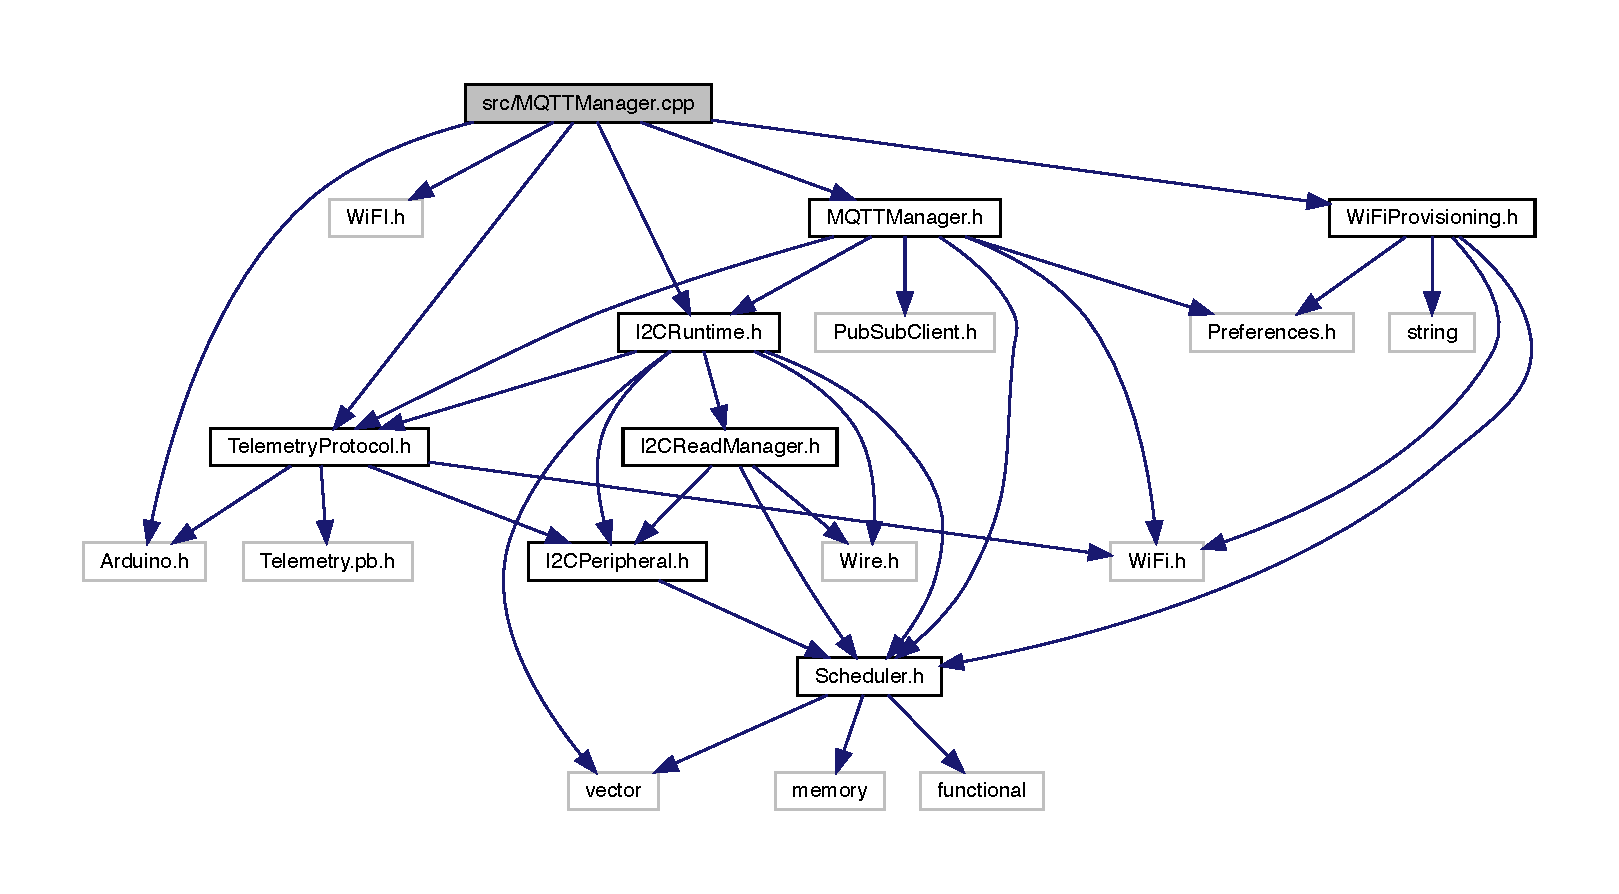
\includegraphics[width=350pt]{_m_q_t_t_manager_8cpp__incl}
\end{center}
\end{figure}

\hypertarget{_scheduler_8cpp}{}\section{src/\+Scheduler.cpp File Reference}
\label{_scheduler_8cpp}\index{src/\+Scheduler.\+cpp@{src/\+Scheduler.\+cpp}}
{\ttfamily \#include $<$Arduino.\+h$>$}\newline
{\ttfamily \#include $<$functional$>$}\newline
{\ttfamily \#include $<$memory$>$}\newline
{\ttfamily \#include $<$vector$>$}\newline
{\ttfamily \#include \char`\"{}Scheduler.\+h\char`\"{}}\newline
Include dependency graph for Scheduler.\+cpp\+:\nopagebreak
\begin{figure}[H]
\begin{center}
\leavevmode
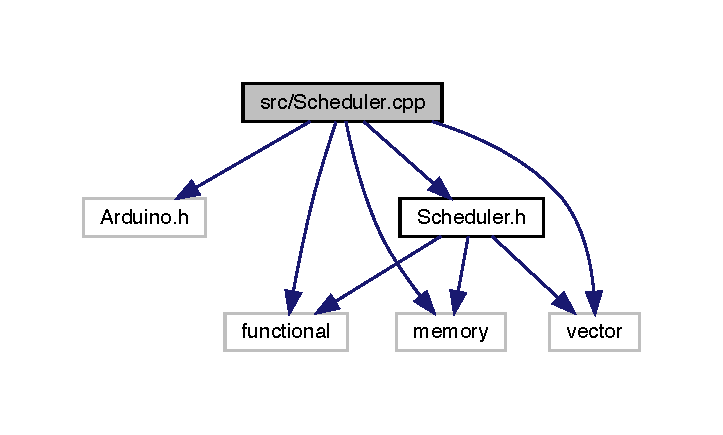
\includegraphics[width=347pt]{_scheduler_8cpp__incl}
\end{center}
\end{figure}

\hypertarget{_telemetry_protocol_8cc}{}\section{src/\+Telemetry\+Protocol.cc File Reference}
\label{_telemetry_protocol_8cc}\index{src/\+Telemetry\+Protocol.\+cc@{src/\+Telemetry\+Protocol.\+cc}}
{\ttfamily \#include $<$Telemetry.\+pb.\+h$>$}\newline
{\ttfamily \#include $<$Wi\+Fi.\+h$>$}\newline
{\ttfamily \#include $<$pb\+\_\+decode.\+h$>$}\newline
{\ttfamily \#include $<$pb\+\_\+encode.\+h$>$}\newline
{\ttfamily \#include $<$vector$>$}\newline
{\ttfamily \#include \char`\"{}I2\+C\+Peripheral.\+h\char`\"{}}\newline
{\ttfamily \#include \char`\"{}Telemetry\+Protocol.\+h\char`\"{}}\newline
Include dependency graph for Telemetry\+Protocol.\+cc\+:\nopagebreak
\begin{figure}[H]
\begin{center}
\leavevmode
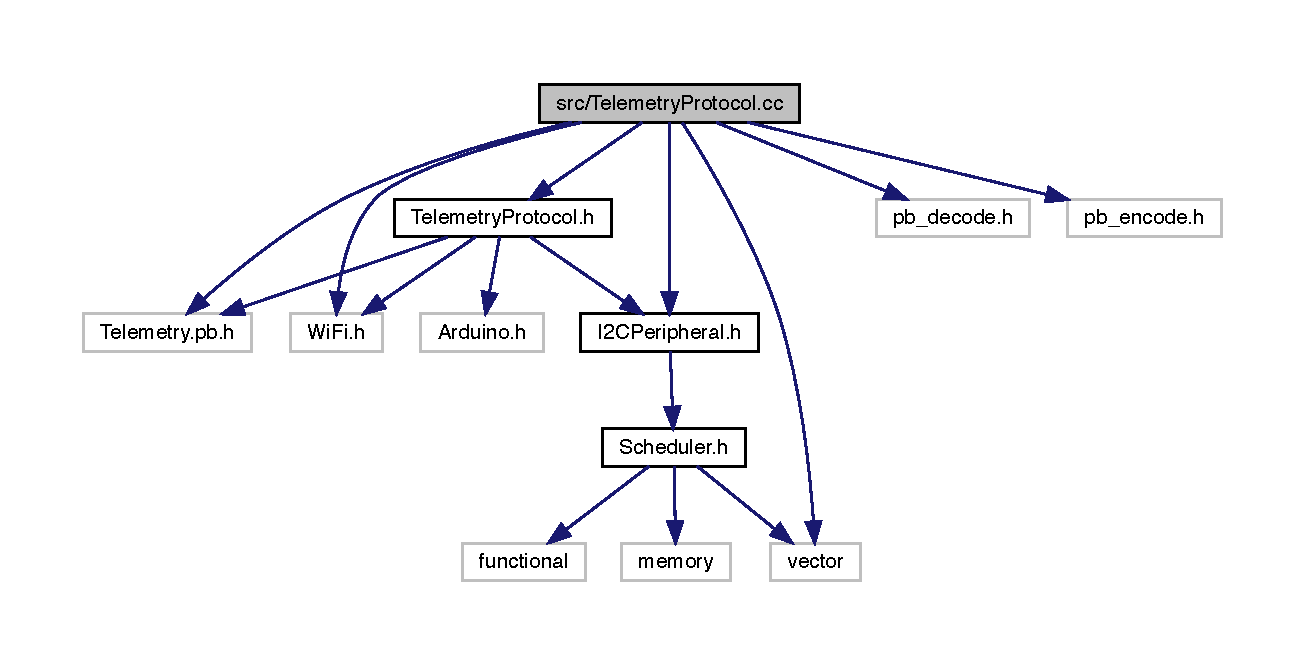
\includegraphics[width=350pt]{_telemetry_protocol_8cc__incl}
\end{center}
\end{figure}
\subsection*{Classes}
\begin{DoxyCompactItemize}
\item 
struct \mbox{\hyperlink{struct_sized}{Sized}}
\begin{DoxyCompactList}\small\item\em Buffer/size pair. \end{DoxyCompactList}\end{DoxyCompactItemize}
\subsection*{Typedefs}
\begin{DoxyCompactItemize}
\item 
typedef struct \mbox{\hyperlink{struct_sized}{Sized}} \mbox{\hyperlink{_telemetry_protocol_8cc_aea229c8162412d1b2d018d2b3cf77356}{Sized}}
\end{DoxyCompactItemize}
\subsection*{Functions}
\begin{DoxyCompactItemize}
\item 
bool \mbox{\hyperlink{_telemetry_protocol_8cc_ab4e6ec2bc915c97e7261fb3cedc19c22}{encode\+\_\+string}} (pb\+\_\+ostream\+\_\+t $\ast$stream, const pb\+\_\+field\+\_\+t $\ast$field, void $\ast$const $\ast$arg)
\item 
bool \mbox{\hyperlink{_telemetry_protocol_8cc_ac526c7d2d7942260c6b09d485dba06e5}{encode\+\_\+statuses}} (pb\+\_\+ostream\+\_\+t $\ast$stream, const pb\+\_\+field\+\_\+t $\ast$field, void $\ast$const $\ast$arg)
\end{DoxyCompactItemize}


\subsection{Typedef Documentation}
\mbox{\Hypertarget{_telemetry_protocol_8cc_aea229c8162412d1b2d018d2b3cf77356}\label{_telemetry_protocol_8cc_aea229c8162412d1b2d018d2b3cf77356}} 
\index{Telemetry\+Protocol.\+cc@{Telemetry\+Protocol.\+cc}!Sized@{Sized}}
\index{Sized@{Sized}!Telemetry\+Protocol.\+cc@{Telemetry\+Protocol.\+cc}}
\subsubsection{\texorpdfstring{Sized}{Sized}}
{\footnotesize\ttfamily typedef struct \mbox{\hyperlink{struct_sized}{Sized}} \mbox{\hyperlink{struct_sized}{Sized}}}



\subsection{Function Documentation}
\mbox{\Hypertarget{_telemetry_protocol_8cc_ac526c7d2d7942260c6b09d485dba06e5}\label{_telemetry_protocol_8cc_ac526c7d2d7942260c6b09d485dba06e5}} 
\index{Telemetry\+Protocol.\+cc@{Telemetry\+Protocol.\+cc}!encode\+\_\+statuses@{encode\+\_\+statuses}}
\index{encode\+\_\+statuses@{encode\+\_\+statuses}!Telemetry\+Protocol.\+cc@{Telemetry\+Protocol.\+cc}}
\subsubsection{\texorpdfstring{encode\+\_\+statuses()}{encode\_statuses()}}
{\footnotesize\ttfamily bool encode\+\_\+statuses (\begin{DoxyParamCaption}\item[{pb\+\_\+ostream\+\_\+t $\ast$}]{stream,  }\item[{const pb\+\_\+field\+\_\+t $\ast$}]{field,  }\item[{void $\ast$const $\ast$}]{arg }\end{DoxyParamCaption})}

\mbox{\Hypertarget{_telemetry_protocol_8cc_ab4e6ec2bc915c97e7261fb3cedc19c22}\label{_telemetry_protocol_8cc_ab4e6ec2bc915c97e7261fb3cedc19c22}} 
\index{Telemetry\+Protocol.\+cc@{Telemetry\+Protocol.\+cc}!encode\+\_\+string@{encode\+\_\+string}}
\index{encode\+\_\+string@{encode\+\_\+string}!Telemetry\+Protocol.\+cc@{Telemetry\+Protocol.\+cc}}
\subsubsection{\texorpdfstring{encode\+\_\+string()}{encode\_string()}}
{\footnotesize\ttfamily bool encode\+\_\+string (\begin{DoxyParamCaption}\item[{pb\+\_\+ostream\+\_\+t $\ast$}]{stream,  }\item[{const pb\+\_\+field\+\_\+t $\ast$}]{field,  }\item[{void $\ast$const $\ast$}]{arg }\end{DoxyParamCaption})}


\hypertarget{_wi_fi_provisioning_8cpp}{}\section{src/\+Wi\+Fi\+Provisioning.cpp File Reference}
\label{_wi_fi_provisioning_8cpp}\index{src/\+Wi\+Fi\+Provisioning.\+cpp@{src/\+Wi\+Fi\+Provisioning.\+cpp}}
{\ttfamily \#include $<$Arduino.\+h$>$}\newline
{\ttfamily \#include $<$Preferences.\+h$>$}\newline
{\ttfamily \#include $<$Wi\+Fi.\+h$>$}\newline
{\ttfamily \#include $<$Wi\+Fi\+A\+P.\+h$>$}\newline
{\ttfamily \#include $<$functional$>$}\newline
{\ttfamily \#include $<$map$>$}\newline
{\ttfamily \#include $<$memory$>$}\newline
{\ttfamily \#include $<$string$>$}\newline
{\ttfamily \#include \char`\"{}Wi\+Fi\+Provisioning.\+h\char`\"{}}\newline
{\ttfamily \#include \char`\"{}index.\+html.\+\_\+cc\char`\"{}}\newline
Include dependency graph for Wi\+Fi\+Provisioning.\+cpp\+:\nopagebreak
\begin{figure}[H]
\begin{center}
\leavevmode
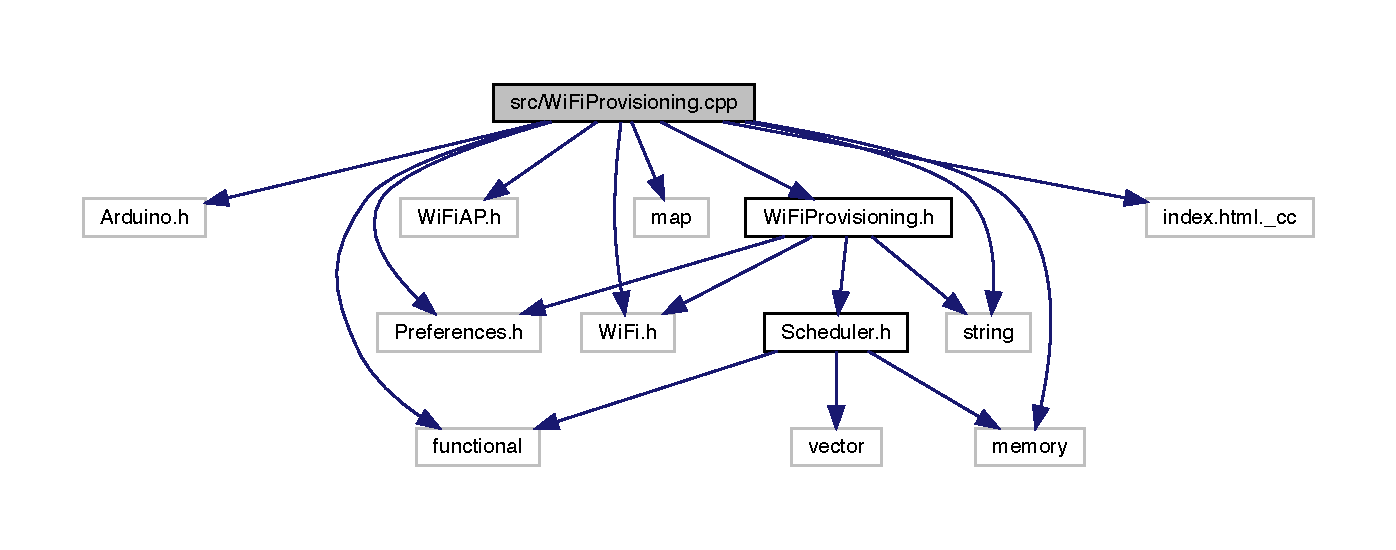
\includegraphics[width=350pt]{_wi_fi_provisioning_8cpp__incl}
\end{center}
\end{figure}
\subsection*{Functions}
\begin{DoxyCompactItemize}
\item 
void \mbox{\hyperlink{_wi_fi_provisioning_8cpp_a15be4380984c85a00d34729245710d4c}{replace}} (std\+::string \&haystack, std\+::string needle, const char $\ast$replacement)
\end{DoxyCompactItemize}


\subsection{Function Documentation}
\mbox{\Hypertarget{_wi_fi_provisioning_8cpp_a15be4380984c85a00d34729245710d4c}\label{_wi_fi_provisioning_8cpp_a15be4380984c85a00d34729245710d4c}} 
\index{Wi\+Fi\+Provisioning.\+cpp@{Wi\+Fi\+Provisioning.\+cpp}!replace@{replace}}
\index{replace@{replace}!Wi\+Fi\+Provisioning.\+cpp@{Wi\+Fi\+Provisioning.\+cpp}}
\subsubsection{\texorpdfstring{replace()}{replace()}}
{\footnotesize\ttfamily void replace (\begin{DoxyParamCaption}\item[{std\+::string \&}]{haystack,  }\item[{std\+::string}]{needle,  }\item[{const char $\ast$}]{replacement }\end{DoxyParamCaption})}


%--- End generated contents ---

% Index
\backmatter
\newpage
\phantomsection
\clearemptydoublepage
\addcontentsline{toc}{chapter}{Index}
\printindex

\end{document}
